\tolerance=10000

     \documentclass[12pt]{report} 

\usepackage{fontenc}
\usepackage{graphicx}
\usepackage{amsmath,amsfonts,bm,bbold}
\usepackage{amssymb}
\usepackage{slashed}

%\usepackage[caption=false]{subfig}
%\usepackage[lofdepth,lotdepth]{subfig}
\usepackage{subfig}
\usepackage{float}
\usepackage[toc]{appendix}
%\usepackage{color}
%\usepackage[usenames,dvipsnames]{color}

\usepackage{setspace}
\usepackage{placeins}
\usepackage{wasysym}
\graphicspath{{/Users/Mike/phdthesis/MY_THESIS/figures/print/}}

%%%%%%%%%%%%%%%%%
\usepackage[sort&compress,numbers]{natbib}
\usepackage[linktocpage=true]{hyperref}
\usepackage{cleveref}

\usepackage[export]{adjustbox}




\usepackage[latin1]{inputenc}
\usepackage{pifont}

\usepackage{graphicx}
\usepackage{epstopdf}
\epstopdfDeclareGraphicsRule{.gif}{png}{.png}{convert gif:#1 png:\OutputFile}
\AppendGraphicsExtensions{.gif}

\usepackage{slashed}
\usepackage{multirow}
\usepackage{booktabs}
\usepackage{ODUthesis}  %%%%%%%%%%%%%
\usepackage{longtable}
\makeatletter
\def\LT@c@ption#1[#2]#3{%
  \LT@makecaption#1\fnum@table{#3}%
  \def\@tempa{#2}%
  \ifx\@tempa\@empty\else
     {\let\\\space
     \addcontentsline{lot}{table}{\protect\numberline{\thetable.}{#2}}}%
  \fi}
\makeatother

%\renewcommand{\theequation}{\arabic{chapter}.\arabic{section}.\arabic{equation}}

%\tablespagefalse

\usepackage[labelsep=period]{caption}

%%%%%%%%%%%%%%%%%%%%%%%%




\begin{document}
%%% new commands and macros %%%%%%%%%%%%%%%%%%%%%%%%%%%%%%%%%%%%%%%%%%%
\newlength{\figwidth}
\setlength{\figwidth}{0.9\columnwidth}

\newlength{\qfigheight}
\setlength{\qfigheight}{0.25\textheight}

\newlength{\hfigheight}
\setlength{\hfigheight}{0.5\textheight}

\newcommand{\dedicationfont}{\fontencoding{T1}\fontfamily{anttlc}\fontseries{m}\fontshape{n}\fontsize{12}{15}\selectfont}

\newcommand{\acro}[1]{#1\@}
\newcommand{\abbr}[1]{\textsc{\texttt{#1}}}
\newcommand{\abbrlc}[2]{\textsc{\texttt{#1}}\texttt{#2}}
\newcommand{\desg}[1]{\texttt{#1}}
\newcommand{\todo}[1]{\textbf{\uppercase{\emph{#1}}}} %\textcolor{Orange}{#1}}}


%Some variables
%
%
\def\g12{\emph{g12}}

\def\G11{\emph{g11}}
\def\clas{\abbr{CLAS }}

\def\Lqcd{\mathcal{L}_{\mathtt{QCD}}}
\def\qfield{\psi}
\def\qbarfield{\overline{\psi}}

\def\grpath{/Users/Mike/phdthesis/MY_THESIS/figures/print}
\def\figures{/Users/Mike/phdthesis/MY_THESIS/figures/print}

\newcommand{\bank}[4]{$\mathtt{#1}^{#2}_{#3}\lbrack\mathtt{#4}\rbrack$}

\def\ith{$i$\textsuperscript{th}}

\def\um{{\text{$\mu$}}m}

%\def\coloronline{(Color online.)\ }
\def\coloronline{}

%%% particles
\def\p{\mathrm{p}}
\def\n{\mathrm{n}}
\def\Kp{\mathrm{K}^{+}}
\def\Km{\mathrm{K}^{-}}
\def\K0{\mathrm{K}^{0}}
\def\Y{\mathrm{Y}}
\def\epos{\mathrm{e}^{+}}
\def\eneg{\mathrm{e}^{-}}
\def\gamstar{\mathrm{$\gamma$}^{*}}
\def\piup{$\pi$}
\def\gammaup{$\gamma$}
%%% TAGGER and RF related times
\def\trf{t_{\mathtt{RF}}}
\def\ttag{t_{\mathtt{TAG}}}
\def\ttagrf{t_{\mathtt{TAG,RF}}}
\def\tprop{t_\mathrm{prop}}
\def\ttrigoffset{t_{\mathrm{trigger-offset}}}

%%% BEAM energy
\def\ebeam{E_{\mathrm{beam}}}

%%% Beta
\def\betasttof{\beta_{\mathtt{ST-TOF}}}
\def\betatof{\beta_{\mathrm{vtx}\mathtt{-TOF}}}
\def\betap{\beta_{p}}

%%% path lengths
\def\lst{\ell_{\mathtt{ST}}}
\def\ltof{\ell_{\mathtt{TOF}}}
\def\lsttof{\ell_{\mathtt{ST-TOF}}}

%%% raw subsystem times
\def\tst{t_{\mathtt{ST}}}
\def\ttof{t_{\mathtt{TOF}}}
\def\dtsttof{\Delta t_{\mathrm{ST-TOF}}}

%%% vertex times
\def\tv{t_{\mathrm{vtx}}}
\def\tvtagrf{t_{\mathrm{vtx}}(\mathtt{TAG_{RF}})}
\def\tvst{t_{\mathrm{vtx}}(\mathtt{ST})}

\def\adcst{\mathtt{ADC}_{\mathtt{ST}}}

\newcommand{\bra}[1]{\left<#1\right|}
\newcommand{\ket}[1]{\left|#1\right>}
\newcommand{\braket}[2]{\left<#1\middle|#2\right>}
\def\piz{$\mathrm{\pi^{0}}\ $}
\def\epem{$e^+e^-\ $}

%%%%%%%%%%%%%%%%%%%%% Publisher's Area please ignore %%%%%%%%%%%%%%%
%

%
%%%%%%%%%%%%%%%%%%%%%%%%%%%%%%%%%%%%%%%%%%%%%%%%%%%%%%%%%%%%%%%%%%%%

\title{Photoproduction of \piz on hydrogen with CLAS from 1.1 GeV - 5.45 GeV using $\lowercase{e}^{+}\lowercase{e}^{-}\gamma$ decay}


\author{Michael C. Kunkel}  

      
        \principaladviser{Moskov Amaryan}
\member{Ian Balitsky}  %This command produces a signature line for the specified member on the
\member{Alex Godunov}  %title page. Use on instance of this command for each member of the
                   %committee other than the advisor up to a total of 5 members.
\member{Chester Grosch} 
\member{Lawrence Weinstein} 


\degrees{M.S. May 2008, Old Dominion University}

\dept{Physics}          %for example \dept{physics}

\submitdate{December 2014}

%\phdfalse          %produces language on title page for Masters Thesis. Otherwise the default
                    %is for a Ph.D. dissertation.

%\copyrightfalse    %suppresses copyright notice

%\figurespagefalse  %suppresses List of Figures

%\tablespagefalse   %suppresses List of Tables

%\vita{The text of the Vita goes here.}


\abstract{Photoproduction of the $\pi^0$ meson was studied using the \textsc{\texttt{CLAS}} detector at the Thomas Jefferson National Accelerator Facility using tagged incident photon energies spanning the range $E_{\gamma}=$~1.1~GeV~-~5.45~GeV. The measurement is performed on a liquid hydrogen target in the reaction $\gamma p\to pe^+e^-(\gamma)$. The final state of the reaction is the sum of two subprocesses for $\pi^0$ decay, the Dalitz decay mode of $\pi^0\to e^+e^-\gamma$ and conversion mode where one photon from $\pi^0\to \gamma\gamma$ decay is converted into a $e^+e^-$ pair. This specific final state reaction avoided limitations caused by single prompt track triggering, while the span of incident photon energies allowed for measurements of $\pi^0$ photoproduction to a domain never systematically measured before.% and allowed a kinematic range extension to the world data on $\pi^0$ photoproduction to a domain never systematically measured before.
\newline \indent We report the measurement of the $\pi^0$ differential cross sections $\frac{d\sigma}{d\Omega}$ and $\frac{d\sigma}{dt}$. The angular distributions agree well with the SAID parametrization for incident beam energies below 3~GeV. As a result with this new data, the $\chi^2/p.d.f.$ of the global fit in the SAID parametrization improved to 3.1 from 3.7. For incident beam energies greater than $3$~GeV a comparison of a model based on Generalized Parton Distributions (\textsc{\texttt{GPD}}) with experimental data shows significant discrepancy, requiring further model developments to describe the data.  %For incident beam energies greater than 3~GeV, a model involving Generalized Parton Distributions (\textsc{\texttt{GPD}}) along with the models predictions are discussed. The comparison of the model to the measurement shows discrepancy, suggesting that the \textsc{\texttt{GPD}} model does not adequately describe the production of $\pi^0$.
% while for an interpretation of the data within the \textsc{\texttt{GPD}} handbag model is discussed for incident beam energies greater than 3~GeV. As a result with this new data, the $\chi^2/p.d.f.$ of the global fit in the SAID parametrization improved to 3.1 from 3.7.}
}




\beforepreface

\prefacesection{Acknowledgements}
%\phantomsection
%\addcontentsline{toc}{section}{Acknowledgments}
%\begin{center}
%    ACKNOWLEDGMENTS
%\end{center}
%
%\vspace{0.75in}
For most of my life, I have been a person with little to say about those that have been part of my inspiration, motivation and education. Since I am a creature of habit, please excuse my forgetfulness and thoughtlessness.\newline  \newline 
Lets start with United States Marine Corps!\\
\indent My greatest accomplishment was proving to myself that I was born a Marine. It has been an honor to know and serve amongst the likes of all my hard-working, hard-hitting, adrenaline junky Teufel Hunden. Stay thirsty my friends and Semper Fi.\\
To the Embry-Riddle Aeronautical University Prescott Campus Physics department of 2007;\\
\indent Dr.~Darrel Smith, Dr.~Nicholas A. Devereux and Dr.~Phillip Anz-Meador, I send you my everlasting gratitude for showing to me that my mind is that of a physicist, displaying overwhelming support on my education and showing patience in teaching. \\
To my colleagues at \abbr{Jlab} ;\\
\indent Dr.~Dennis Weygand, Dr.~Michael Paolone, and Dr.~Johann Goetz, the patience you have shown me is unprecedented. You have taught me the tools I needed to \emph{debug debug debug}, perform outstanding analyses and even though we agreed on nothing but science, we are still able to be great colleagues.\\
To the Old Dominion University Physics department;\\
\indent Dr. Lawrence Weinstein, thank you for showing support throughout my studies and being a rock of knowledge. \\
\indent Dr. Anatoly Radyuskin, you are always a source of well placed meaningful knowledge along a sense of humor. I thank you for all of our conversations and laughs. \\
\indent Dr. Moskov Amaryan, there are no words that I can muster to properly convey what I would like to write about the time you were my advisor. A few underrated words would be \emph{lucky}, \emph{indebted}, \emph{kindness}, \emph{patience}, and not to mention \emph{frustrating}. However, I believe the greatest thing you have taught me comes from one of your many analogies in which you stated, ``Michael, have patience, you cannot change ones rest frame.''\\
To My family; \\
Dr. Asl\i \ Tando\u{g}an my loving wife. I was smitten the first day I met you and I have been smitten with you everyday afterward. You are a great source of my happiness. I look forward to all the hard work and dedication we will input into our lives with the reward of companionship and love. Thank you for your support and honestly you have given throughout this endeavor we both have undertaken. \\
Michael-\c{C}\i nar Kunkel and future sons and daughters. When there is something you want to achieve in life, you must first understand the terrain to achievement, be willing to take necessary detours, be steadfast in your commitments, be intelligent with your falls, never be afraid to fail, and never settle for anything less than sixth gear pinned wide open. These guidelines might appear to be a lengthy list of nonsense, but throughout my life I have held onto these as if they were virtues. I have won, I have lost, I have smiled and I have pouted but I climbed my pinnacles, if only to gaze onto other crags. Whichever paths you choose, remember that ``Baba might not know, but Baba knows.''

\clearpage

\prefacesection{Dedication}
%\pdfbookmark[1]{Dedication}{dedication}
\begin{center}
\quad \\

\vspace{2in}

\begin{minipage}{0.8\columnwidth}
\begin{center}
{\dedicationfont%
This dissertation is dedicated to my fellow Belleau Woodsman,\\
brother \\ SSGT Christopher Michael Zimmerman USMC \\ 04/01/1978 - 09/20/2006 KIA Afghanistan. \\
I can imagine a life in which you and I would discuss the meaning of me receiving a doctorate in physics. This conversation probably ends with me saying to you "True, I am an assclown but now I am thee assclown." to which you would jovially reply with "Still an assclown though. Now pass me the tap". \\
%For if we were to ever have one of our wonderful spats again, it would end with me saying to you "True, I am an assclown but now I am thee assclown." to which I can imagine you jovially replying with "Still an assclown though. Now pass me the tap". \\
Semper Fidelis }
\end{center}
\end{minipage}

\end{center}
\clearpage

\afterpreface
%\setcounter{chapter}{0}
%\setcounter{secnumdepth}{-1}

\chapter{Introduction and Motivation}\label{sec:intro}
The goal of this analysis is to provide insight into the mechanisms, baryon resonances and productions channels involved in \piz production for incident beam energies already explored as well as for incident beam energies in which there exists only a sparse and in some cases no amount of data.
Nucleons are composite particles, meaning they are made up of smaller constituents. To gain insight into the structure of the nucleon, physics employ baryon spectroscopy to explore for baryon resonances. Experimental, theoretical and phenomenological methods have been developed to refine and expand the known resonance masses, widths, and electromagnetic couplings~\cite{Dugger07}. Precise measurements of the cross-section and polarization asymmetries are important to extract photo-decay amplitudes and production mechanisms. Recently there has been improvement in Wide Angle Compton Scattering predictions using a General Parton Distribution (\abbr{GPD}) handbag model. This framework has also been recently adopted into \piz production~\cite{Huang2000} to describe the production as single quark excitation in photon-quark scattering.
%of   in which the production of the nucleons is considered in a 2 part soft and hard mechanism exchange.

In this analysis, we report on an experiment that was performed with the Cebaf Large Angle Spectrometer (\abbr{CLAS}) setup at the Thomas Jefferson National Accelerator Facility (\abbr{TJNAF}). The experiment used a tagged photon beam produced via bremsstrahlung from a 5.715~GeV electron beam delivered from the CEBAF accelerator. The photon beam struck a liquid hydrogen target. The reaction of interest is photoproduction of neutral pions on a hydrogen target, $\gamma p\to p\pi^0$, with subsequent Dalitz decay $\pi^0\to e^+e^-\gamma$ or standard decay plus photon conversion conversion mode $\pi^0\to \gamma\gamma\to e^+e^-\gamma$ . Neither the Dalitz decay mode of $\pi^0$ with very small branching ratio of $\sim 1.2\%$, nor the conversion mode from the main decay mode $\pi^0\to \gamma\gamma$ with branching ratio $\sim 98.8\%$ is preferred. The conversion rate of $\gamma$ to $e^+e^-$ is substantial enough that the Dalitz and the conversion process share the total statistical sample. The cross-section measurement is performed for the reaction $\gamma p\to pe^+e^-(\gamma)$ using a tagged photon beam spanning the energy interval  $E_{\gamma}=1.142$~GeV$-5.425$~GeV. In the final state of the reaction the photon is missing, $p e^+e^-$ are detected and $\pi^0$ is identified in the missing mass of the proton.

Using \epem decay products of \piz, contrary to $\gamma\gamma$ decay of \piz, along with detection of the proton allowed the experiment to run with high current. This was achieved by requiring a trigger configuration comprised of multiple charged tracks along with Cherenkov and Electromagnetic Calorimeter detection for photon beam energies $1.142$~GeV$ < E_{\gamma} < 3.6$~GeV. For photon beam energies greater than $3.6$~GeV a trigger configuration comprised of just multiple charged tracks was utilized.
\FloatBarrier
%
%
%
%
%. First we wanted to study $M_{e+e-}$ dependence of $\pi^0$ cross section, secondly and most importantly in the Dalitz decay mode final state contains three charged tracks, contrary to $\gamma\gamma$ decay, which allows to run experiment with high current, which otherwise wouldn't have been possible with single prong charged track, due to trigger and data acquisition limitations.
%\setcounter{secnumdepth}{2}
\section{Hadrons}
In the quark model, a hadron is a colorless particle formed of quarks and anti-quarks that are bound together by the strong force. Hadrons are organized and classified according to their quark content. The standard model permits multiple valence quark configurations for hadrons, however to date only two configurations have been verified, baryons and mesons. Baryons are hadrons with three quarks with suitable colors, while hadrons with two valence quarks, a quark and an anti-quark with color and ``anti-color'', are called mesons. Since baryons have an odd number of valence quarks, they are spin $\frac{1}{2}$ particles and thus are fermions, however mesons are spin 0 or 1 particles are bosons. As in any quantum-mechanical bound system, the valence quarks have a discrete energy level spectrum due to the various modes of the di-quark excitations, vibrations, orientations and vibrations which give rise to the quantum numbers $J^{PC}$. Here $J=L+S$ is defined as the total angular momentum containing orbital angular momentum $L$ and spin $S$, while $P=(-1)^{L+1}$ and $C= (-1)^{L+S}$ are defined as parity and charge conjugation.
% 
%The valence quarks in hadrons produce the quantum numbers $J^{PC}$, where $J=L+S$ is the total angular momentum created by the orbital angular momentum, L,  and the spin, S, of the particle. The ``P" stands for parity, $P = (-1)^{L+1}$, and ``C" is the charge conjugation, $C = (-1)^{L+S}$. Each type of meson can be categorized by their spin configuration and are shown in table 1 below.
% 
% 
%In the quark model, mesons are comprised of two valence quarks which are a quark and an anti-quark with color and ``anti-color''. Since mesons are comprised of a quark-antiquark pair, they are bosons. 
%These various modes give rise to the quantum numbers of the mesons via their flavor and symmetry $J^{PC}$.
%The different mesons can be classified into types according to their spin configurations. 
Each type of meson can be categorized by their spin configuration and are shown in Tab.~\ref{tab:meson_type}.
\begin{table}
\begin{minipage}{\textwidth}
\begin{center}
\begin{singlespacing}

\caption[Types of mesons]{\label{tab:meson_type}Types of mesons}

\begin{tabular}{c c c c c c} % centered columns (4 columns)
\hline%inserts double horizontal lines
Type & J & P & L & S & J$^{P}$ \\ [0.5ex] % inserts table
%heading
\hline % inserts single horizontal line
Pseudoscalar & 0 & - & 0 & 0 & 0$^-$\\
Scalar & 0 & + & 1 & 1 & 0$^+$\\
Vector & 1 & - & 0 & 1 & 1$^-$\\
Axial Vector & 1 & + & 1 & 0 & 1$^+$\\
Tensor & 2 & + & 1 & 1 & 2$^+$ \\ [1ex]
\hline \hline%inserts single line
\end{tabular}

\end{singlespacing}
\end{center}
\end{minipage}
\end{table}
\vspace{20pt}


%\begin{tabular}{c||c|c|c|c||c}
%Type & $S$ & $L$ & $P$ & $J$ & $J^P$ \\ \hline \hline
%Pseudoscalar meson & 0 & 0 & - & 0 & $0^-$\\ \hline 
%Axial vector meson & 0 & 1 & + & 1 & $1^+$\\ \hline 
%Vector meson & 1 & 0 & - & 1 & $1^-$\\ \hline 
%Scalar meson & 1 & 1 & + & 0 & $0^+$\\ \hline 
%Tensor meson & 1 & 1 & + & 2 & $2^+$
%
%
%\end{tabular}
\FloatBarrier

\subsection{Light Pseudoscalar Mesons} 
The following analysis will concentrate on the lightest neutral pseudoscalar meson, $\pi^0$, which is member of the family of $P_p$($\pi^{0}, \eta, \eta'$)($J^{P}=0^{-}$) mesons that are subject to U(3) flavor symmetry. The nonet, the resulting nine states that can be decomposed into a singlet and an octet state, of the pseudoscalar mesons are seen in Fig.~\ref{fig:nonet.pseud}, where strangeness increases upward on the page and charge increases toward the right side of the page.
\begin{figure}[h!]\begin{center}
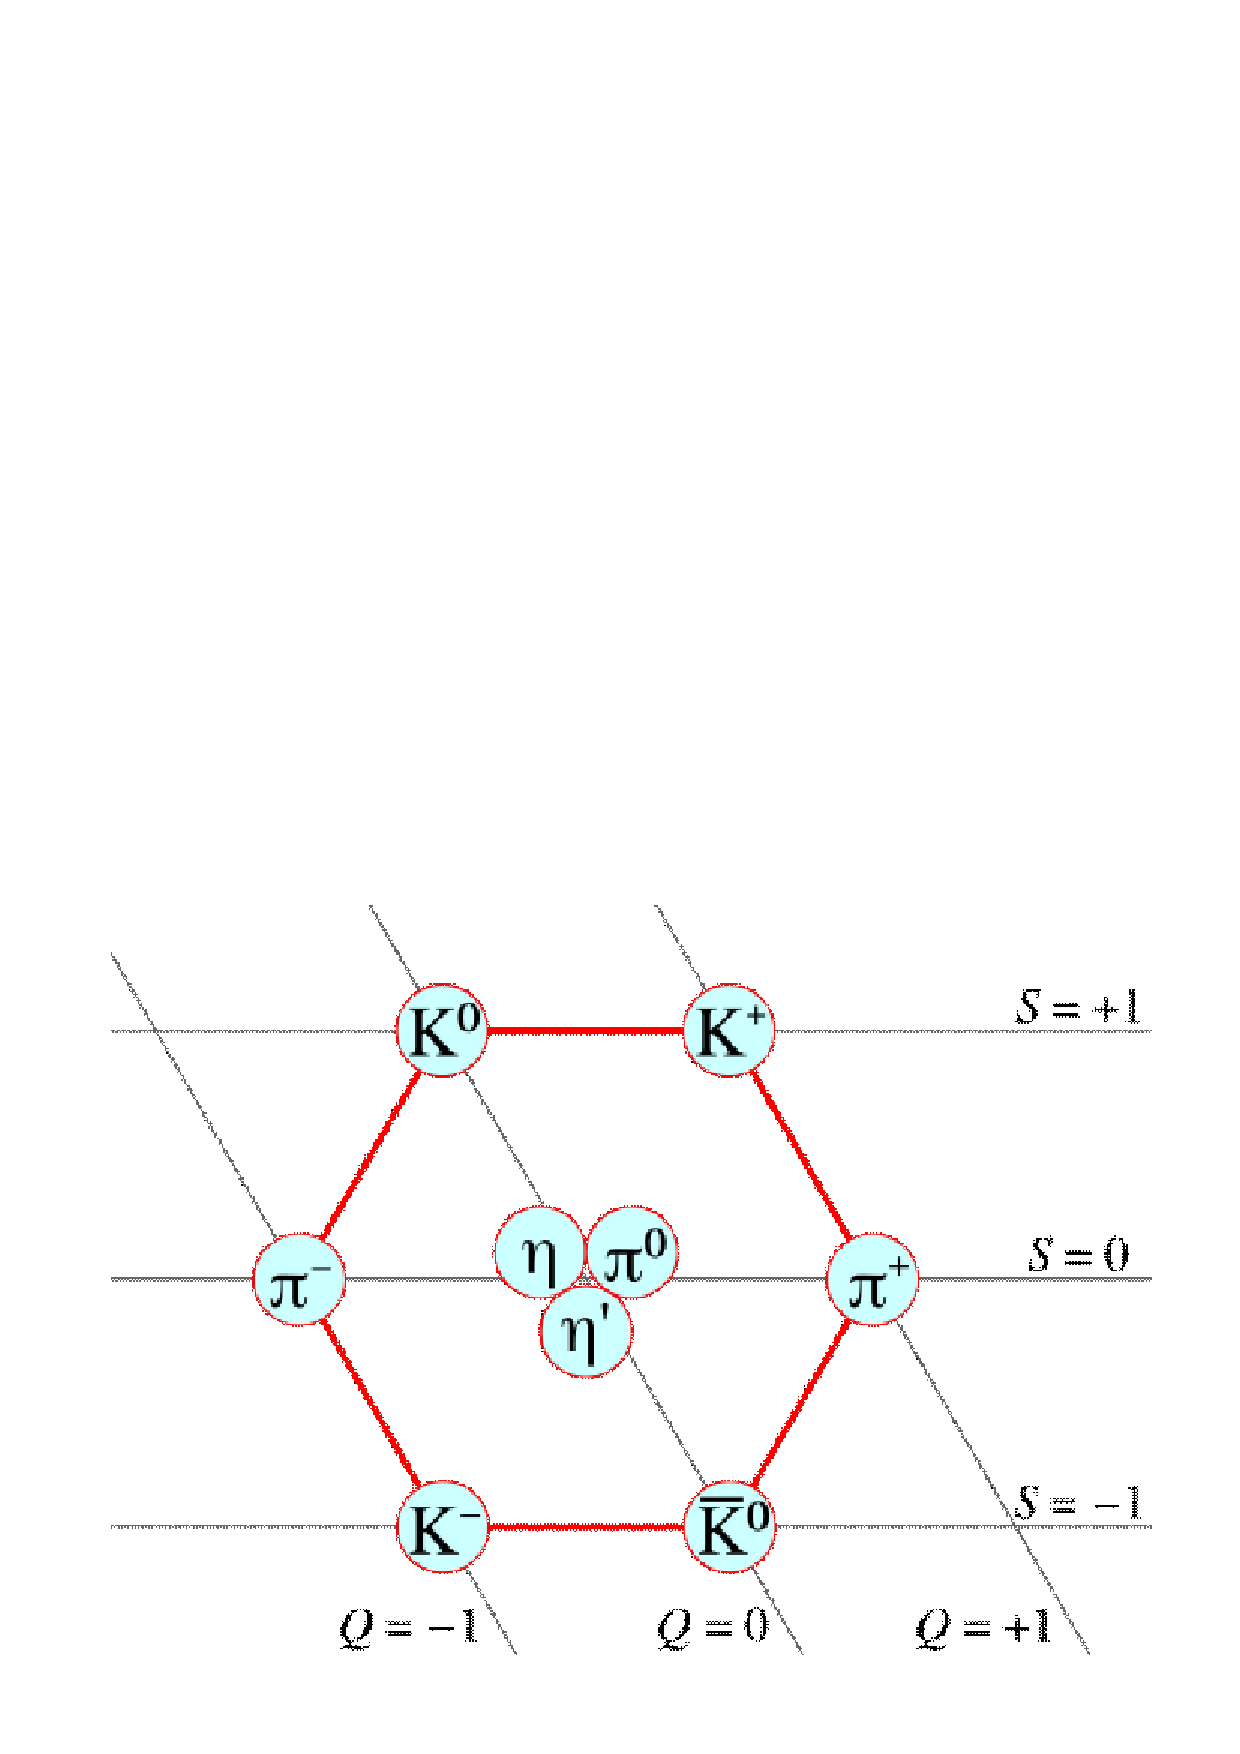
\includegraphics[width= 0.8 \figwidth ,height=\qfigheight]{\grpath/intro/pseudoscalar.pdf}
\caption[Nonet of Pseudoscalar Mesons]{\label{fig:nonet.pseud}Nonet of Pseudoscalar Mesons~\cite{wiki1}.}
\end{center}\end{figure}
It should be noted that the $\eta$ and $\eta'$ are not exact octet ($\eta_{8}$) and singlet ($\eta_{0}$) states, as they are linear combinations of $\eta_{8}$ and $\eta_{0}$ according to:
\begin{eqnarray}
\left(
\begin{array}{cc}
\eta \\
\eta ' 
\end{array}
\right)
& = &
\left(
\begin{array}{cc}
-\sin\theta_{mix} & \cos\theta_{mix} \\
\cos\theta_{mix} & \sin\theta_{mix}
\end{array}
\right)
\cdot
\left(
\begin{array}{cc}
\eta_{0} \\
\eta_{8}
\end{array}
\right)
\end{eqnarray}
where $\theta_{mix} = -18.6^{\circ}$\cite{Goity} and $\eta_{8}$ and $\eta_{0}$  have quark content of:
\begin{eqnarray}
\eta_{0} &\rightarrow & \sqrt{\frac{1}{6}}(u\overline{u} + d\overline{d} +  s\overline{s})\nonumber\\
\nonumber \\
\eta_{8} &\rightarrow & \sqrt{\frac{2}{3}}(u\overline{u} + d\overline{d} - 2s\overline{s})\nonumber \\
\nonumber \\
\nonumber 
\end{eqnarray}
The physical masses of $\eta$ and $\eta'$ are $m_{\eta} = 547.51\pm 0.18$~MeV \cite{pdg2014}, $m_{\eta'} =957.78 \pm 0.14$~MeV \cite{pdg2014}, and the widths are $\Gamma_{\eta} =1.30\pm0.07$~keV and $\Gamma_{\eta'} = 0.203\pm0.016$~MeV.
The lightest of the mesons $\pi^{0}$ has a quark content of:
\begin{eqnarray}
\pi^{0} = \frac{1}{\sqrt{2}}(u\overline{u} - d\overline{d})\nonumber
\end{eqnarray}
and mass of $m_{\pi^{0}} = 134.9766 \pm 0.0006$~MeV \cite{pdg2014}. The decay modes for \piz are given in Table \ref{tab:pi0}.
\begin{table}
\begin{minipage}{\textwidth}
\begin{center}
\begin{singlespacing}

\caption[Branching Ratios of the \piz Decay]{\label{tab:pi0} Branching ratios of the \piz decay.~\cite{pdg2014}}
\begin{tabular}{l|c}
\hline												
Mode	& Branching ratio \\ \hline 	
$\pi^0 \to 2\gamma$	 &   $ (98.823 \pm 0.034)  \cdot 10^{-2}$ \\	
$\pi^0 \to e^+ e^-\gamma$  &  $  (1.174 \pm 0.035)  \cdot 10^{-2}$ \\
$\pi^0 \to \gamma $ positronium   &  $ (1.82 \pm 0.29)  \cdot 10^{-9}$\\
$\pi^0 \to  e^+ e^+ e^- e^-	$  &  $( 3.34 \pm 0.16)  \cdot 10^{-5}$\\
$\pi^0 \to  e^+ e^-$  &  $ (6.46 \pm 0.33)  \cdot  10^{-8}$\\
$\pi^0 \to 4\gamma$	&  $<2 \cdot 10^{-8}$\\
$\pi^0 \to \nu \bar \nu$  &  $<2.7 \cdot 10^{-7}$\\
$\pi^0 \to \nu_e \bar \nu_e$  &  $<1.7 \cdot 10^{-6}$\\
$\pi^0 \to \nu_{\mu} \bar \nu_{\mu}$  &  $<1.6 \cdot 10^{-6}$\\
$\pi^0 \to \nu_\tau \bar \nu_\tau $  &  $<2.1 \cdot 10^{-6}$\\
$\pi^0 \to \gamma \nu \bar \nu$	 &  $<6 \cdot 10{-4}$\\
\hline \hline%inserts single line
\end{tabular}

\end{singlespacing}
\end{center}
\end{minipage}
\end{table}
\vspace{20pt}

%\begin{figure}[h!]\begin{center}
%\subfloat[Nonet of Pseudoscalar Mesons][]{ %Feynman diagram of \piz two photon decay
%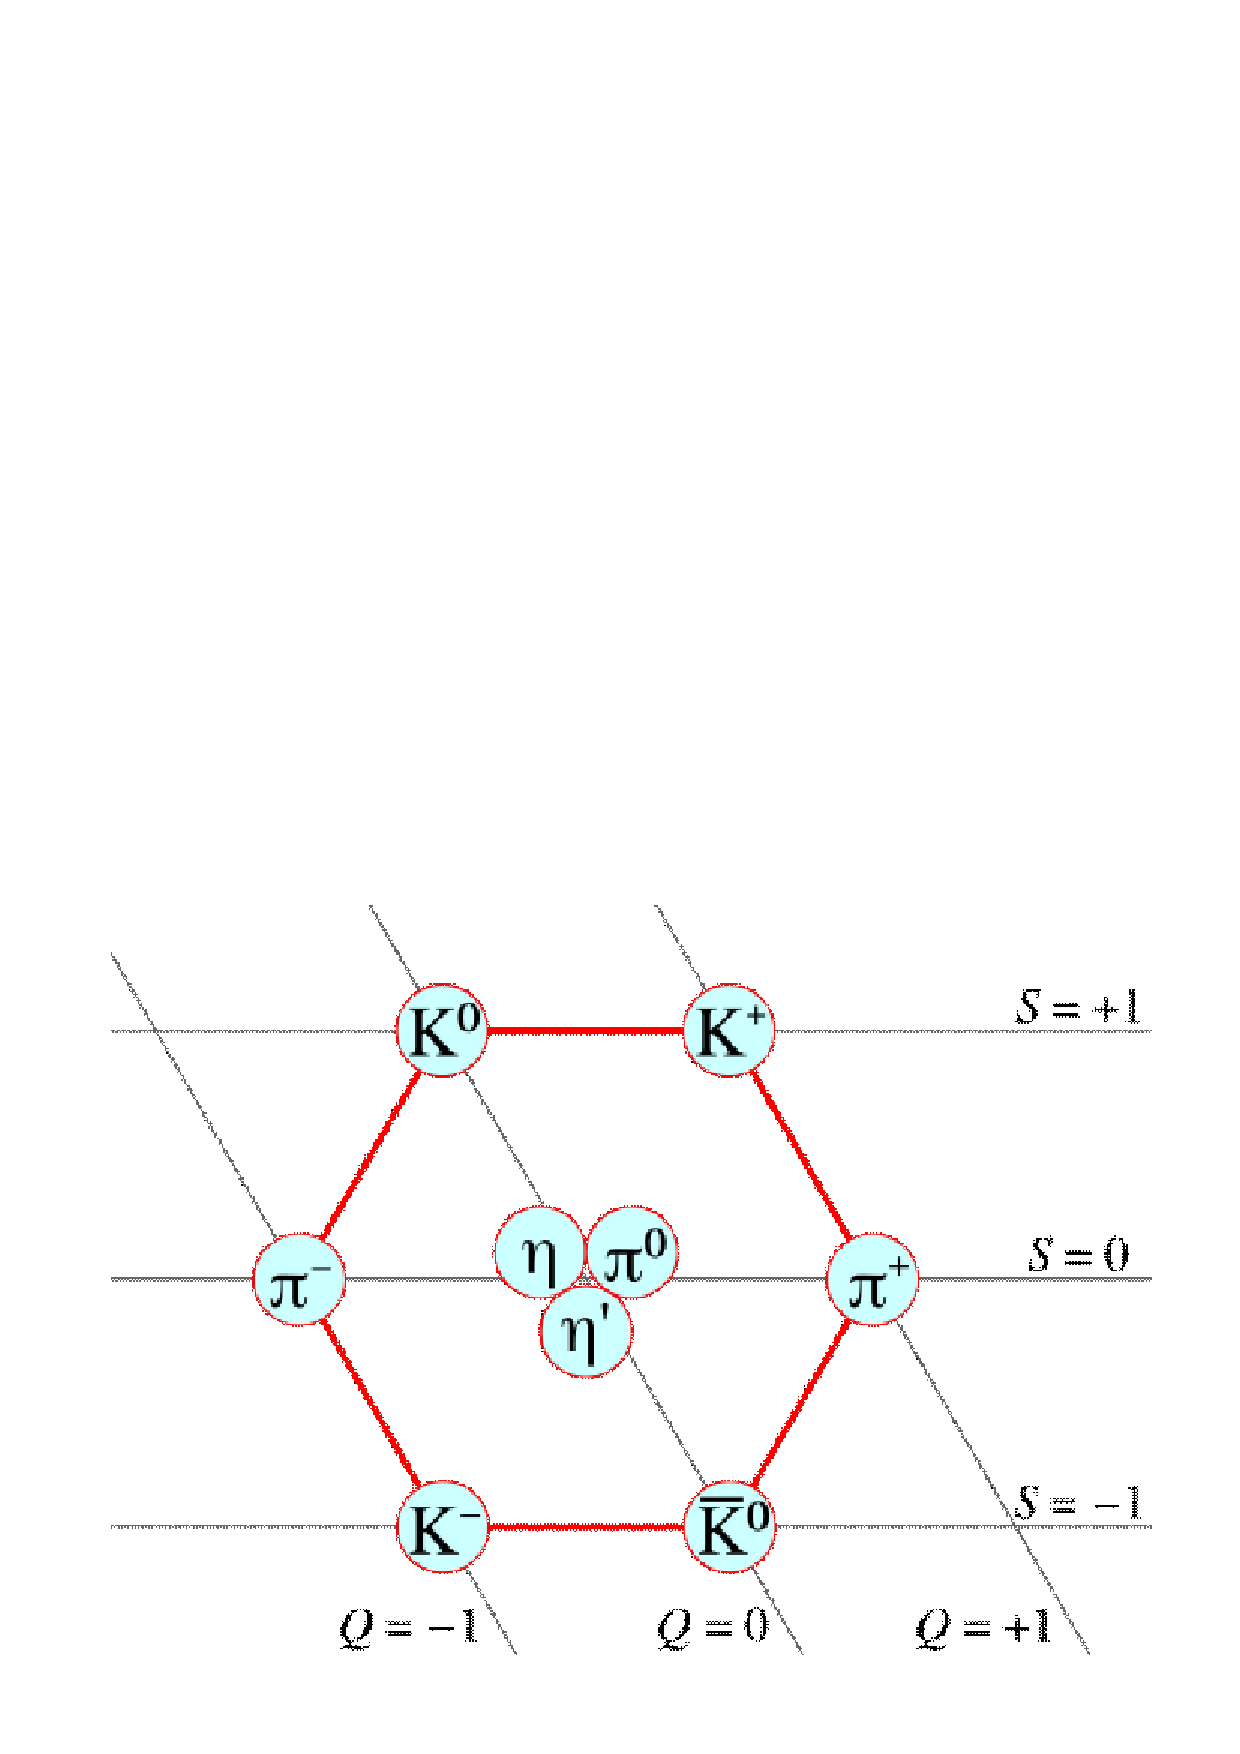
\includegraphics[width=0.65\columnwidth,height=0.5\qfigheight]{\grpath/intro/pseudoscalar.pdf}\label{fig:nonet.pseud}
%}
%
%\subfloat[Nonet of Vector Mesons][]{ %Feynman diagram of \piz Dalitz decay
%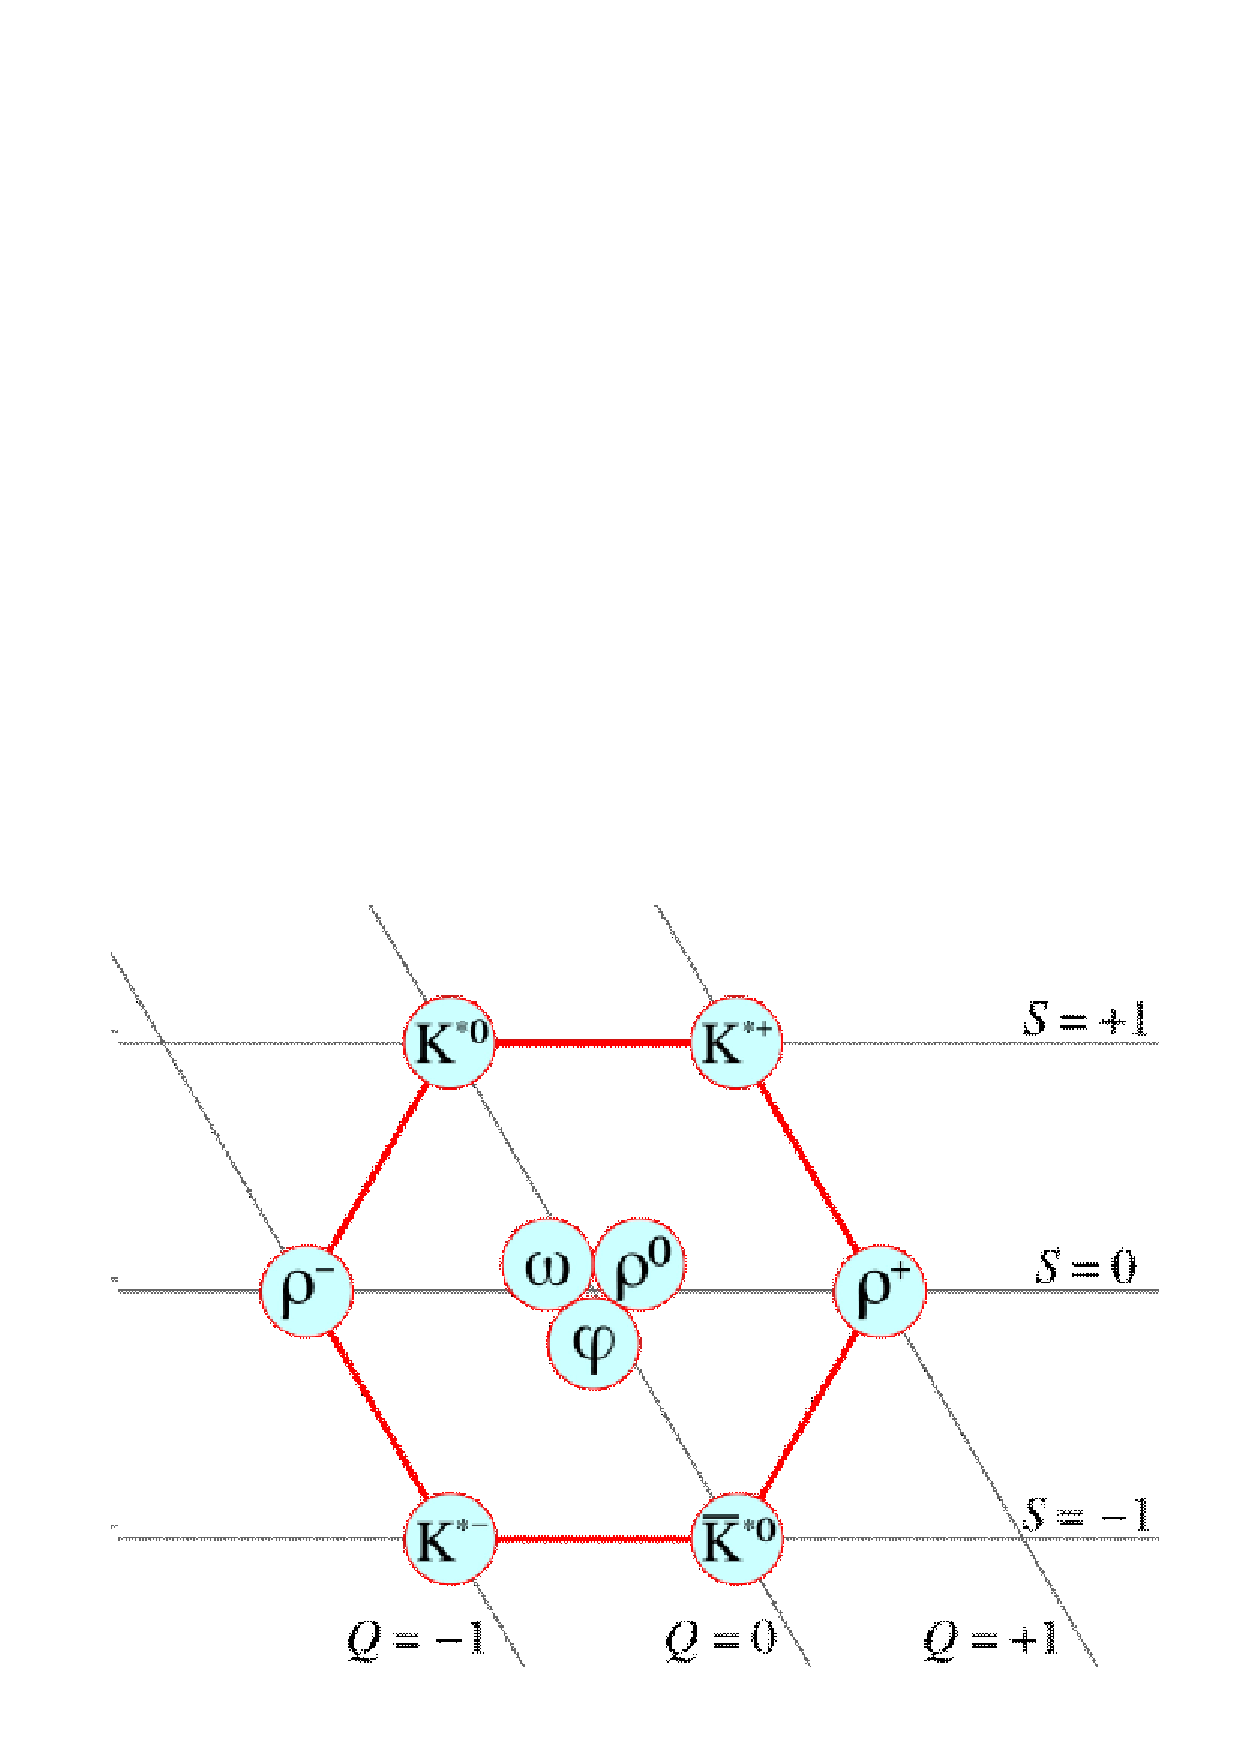
\includegraphics[width=0.65\columnwidth,height=0.5\qfigheight]{\grpath/intro/vector.pdf}\label{fig:nonet.vect}
%}
%\caption[Nonet of Pseudoscalar and Vector Mesons]{\label{fig:piz.alldecay}Nonet of pseudoscalar mesons~\subref{fig:nonet.pseud}. Nonet of vector mesons~\subref{fig:nonet.vect}.}
%
%\end{center}\end{figure}
%
%The \piz is the lightest meson with a mass of $m_{\pi^0}= (134.9766 \pm 0.0006) {\rm MeV}$ \cite{pdg2014}. The quark content is:
%\begin{equation}
% \pi^0 : \frac{1}{\sqrt{2}}\left(u \bar u  - d \bar d \right).
%\end{equation}

%In the intended analysis, it is planned to investigate the cross-section of the \piz.

\section{\piz Production} \label{sec:into:xsection}
The present analysis uses two approaches to describe the behavior of the \piz cross-section. One approach is for incident photon beam energies less than 2.8~GeV where the missing resonance search is most valid and the data can be described well by coupling of the \piz electromagnetic wave functions. The second approach attempts to describe the behavior of the \piz by using General Parton Distribution models, \abbr{GPD} for incident photon beam energies greater than 2.8~GeV.
%The physics behind this is that since the photon couples to charged-fermion pairs, a part of its cross-section could be described by considering interactions between the hadron and a virtual fermion pair~\cite{butterworth}.


\subsection{Low Energy \piz Production}\label{sec:into:xsection.low}

\begin{figure}[h!]\begin{center}
\includegraphics[width=0.5 \figwidth,height= \qfigheight]{\figures/feyman_pi0IV.pdf}
\caption[Diagram for photoproduction of the \piz meson]{\label{fig:xsection.pi0feynman}	Diagram for photoproduction of the \piz meson. $k$ and $p_i$ are the incident photon beam and target proton 4-moment respectively, $q$ and $p_f$ represent the produced \piz meson and scattered proton 4-momenta respectively.}
\end{center}\end{figure}
For incoming photon beam energies less than 2.8~GeV, the production of the \piz meson, with 4-momenta $q$, in photon-proton reactions, with 4-momenta $k$ and $p_i$ respectively and $p_f$ being the 4-momenta of the scattered proton (see Fig.~\ref{fig:xsection.pi0feynman}),  can be described in terms of the three Lorentz invariant Mandelstam variables, $s$, $t$ and $u$, where
\begin{align}
s = (k+p_i)^2 = (q+p_f)^2 \nonumber \\
t=(p_i-p_f)^2 = (k-q)^2  \nonumber \\
u = (k - p_f)^2 = (p_i-q)^2 \ .
\end{align}
The sum of the Mandelstam variables linearly combine to give the sum of masses of the particles involved:
\begin{align}
s + t + u = \sum\limits_{i}^{4} m_i^2 
\end{align}
and the definition of Lorentz-invariant mass:
\begin{align}
p_i\cdot p_i = E_i^2 - \mathbf{p_i}\cdot \mathbf{p_i} = m_i^2 \ .
\end{align}
Using energy-momentum conservation:
\begin{align}
k + p_i = q+p_f \,
\end{align}
it is seen that only three of the four momenta are independent. Conventionally the use of $k$ and $q$ and a combined 4-momenta of the nuclei 
\begin{align}
P = \frac{1}{2}(p_i+p_f)
\end{align}
are used as the independent kinematic variables. The three Mandelstam variables can be express in terms of the other two, therefore the scattering process is described by functions of only two of the Mandelstam variables. Conventionally they are chosen to be $s$ and $t$, which in the center-of-mass frame (C.M.) of the initial and final state equal the invariant mass squared of the system and the momentum transfer in the production process respectively.
\subsection{Isospin Representation}\label{sec:isospin}
The scattering matrix $\mathcal{M}$ for single pion photoproduction process is written as:
\begin{align}
\mathcal{M} =  (\epsilon_\mu k_\nu - \epsilon_\nu k_\mu)&[ \frac{1}{2}i \gamma_5 \gamma_\mu \gamma_\nu A_1(s,t) + 2 i \gamma_5 P_\mu(q-\frac{1}{2}k)_\nu A_2(s,t) \nonumber \\ & + \gamma_5 \gamma_\mu q_\nu A_3(s,t) + \gamma_5 \gamma_\mu(2P_\nu- i M\gamma_\nu) A_4(s,t) ] \ ,
\end{align}
where $M$ is the nucleon mass, $\epsilon$ is the photon polarization and $A_i(s,t)$ are the invariant functions of the Mandelstam invariants $s$ and $t$. The amplitude $A_i(s,t)$ refers to the emission of a pion of isospin index $\alpha$, and is given by the well-known formula:
\begin{align}\label{eq:isoscal_vec}
A_i(s,t)= A_i^{(0)}\tau_\alpha + A_i^{(+)}\delta_{\alpha 0} + \frac{1}{2} A_i^{(-)}\left[\tau_\alpha,\tau_0\right] \ ,
\end{align}
where $\tau_\alpha$ are the nucleon isospin transition operators, where the sign of $\alpha$ indicates the opposite sign of the pion isospin, this is by convention. Eq.~\ref{eq:isoscal_vec} assumes that the photon interaction with hadrons occurs through isoscalar and isovector parts, so that $A_i^{(0)}$ is the isoscalar amplitude that corresponds to a zero net isospin transistion resulting from the electromagnetic field. The amplitudes $A_i^{(+)}$ and $A_i^{(-)}$ are the isovector amplitudes and can be combined as $A_i^{(+)} + 2 A_i^{(-)}$ and $A_i^{(+)} - A_i^{(-)}$ so that the pion nucleon final state has definite isospin $\frac{1}{2}$ and $\frac{3}{2}$ respectively~\cite{Rosenfeld} by use of
\begin{align}
A^S = -(3)^\frac{1}{2}A^{(0)} \nonumber \\
A^{V1} = \left(\frac{1}{3}\right)^\frac{1}{2}A_i^{(+)} + 2 A_i^{(-)} \nonumber \\
A^{V2} = \left(\frac{2}{3}\right)^\frac{1}{2}A_i^{(+)} - A_i^{(-)} \ ,
\end{align}
where $A^S$, $A^{V1}$ and $A^{V2}$ are the isoscalar amplitude, isovector amplitude of isospin $\frac{1}{2}$ and isovector amplitude of isospin $\frac{3}{2}$ respectively.
The four possible pion nucleon amplitudes $A_i(s,t)$ of the initial and final state particles in the pion photoproduction process are in terms of the isoscalar and isovector are:
\begin{align}
A_1(\gamma p \to n \pi^+) = -\sqrt{\frac{1}{3}}A^{V3} + \sqrt{\frac{2}{3}}(A^{V1} - A^{S}),\\
A_2(\gamma p \to p \pi^0) = \sqrt{\frac{2}{3}} A^{V3} + \sqrt{\frac{1}{3}}(A^{V1}-A^{S}),\\
A_3(\gamma n \to p \pi^-) = \sqrt{\frac{1}{3}}A^{V3} - \sqrt{\frac{2}{3}}(A^{V1} + A^{S}),\\
A_3(\gamma n \to n \pi^0) = \sqrt{\frac{2}{3}}A^{V3} + \sqrt{\frac{1}{3}}(A^{V1} + A^{S}).
\end{align}
Since the combination $\sqrt{\frac{2}{3}}(A^{V1} \mp A^{S})$ gives the coupling of photons to positive and neutral isospin-$\frac{1}{2}$ states, respectively, ~\protect\cite{Rosenfeld}, defined explicitly
%
\begin{align}
&&A^p = + \sqrt{\frac{2}{3}}(A^{V1} - A^{S}),\\
&&A^n = -\sqrt{\frac{2}{3}}(A^{V1} + A^{S}).
\end{align}
\subsection{Structure Functions}\label{sec:CGLN}
To obtain the scattering matrix elements in terms of experimental quantities, it is preferred and easier to work in the C.M. system and reduce the $\mathcal{M}$ to a form $\mathcal{F}$ by equating the invariant form of the scattering matrix elements in each frame, i.e.:
\begin{align}
\bar{u}(p_2)\mathcal{M} u(p_1) \equiv \frac{4 \pi W}{M}\chi_f^\dagger \mathcal{F} \chi_i \ ,
\end{align}
where $\bar{u}(p_2)$ and $u(p_1)$ are final and initial state Dirac spinors respectively and $\chi_f$ and $\chi_i$ are final and initial state Pauli spinors. The differential cross-section for single pion production is:
\begin{align}
\frac{d\sigma}{d\Omega} = \frac{q}{k}| \bra{f}\mathcal F \ket{i}|^2,
\end{align}
The expression to express Dirac spinors in terms of Pauli spinors is written as:
\begin{align}
\mathcal{F} = & i\vec{\mathbf{\sigma}}\cdot \vec{\mathbf{\epsilon}} \mathcal{F}_1 + \frac{1}{qk}(\vec{\mathbf{\sigma}}\cdot \vec{\mathbf{q}})\vec{\mathbf{\sigma}} \cdot(\vec{\mathbf{k}}\times \vec{\mathbf{\epsilon}}) \mathcal{F}_2 \nonumber \\ & + \frac{i}{qk}(\vec{\mathbf{\sigma}}\cdot \vec{\mathbf{k}})(\vec{\mathbf{q}}\cdot \vec{\mathbf{\epsilon}})\mathcal{F}_3 + \frac{i}{q^2}(\vec{\mathbf{\sigma}}\cdot \vec{\mathbf{q}})(\vec{\mathbf{q}}\cdot \vec{\mathbf{\epsilon}})\mathcal{F}_4 \ ,
\end{align}
where $\vec{\mathbf{k}}$ and $\vec{\mathbf{q}}$ are the C.M. 3-momenta and $\vec{\mathbf{\epsilon}}$ is the polarization of the photon. The relationship between $A_i$ and $\mathcal{F}$ is found using the relations:
\begin{align}
\mathcal{F}_1 = \frac{W- M}{8 \pi W }(D_1 D_2)^{\frac{1}{2}}\left[ A_1+(W-M)A_4 - \frac{k_0q_0-\vec{\mathbf{k}}\cdot \vec{\mathbf{q}}}{W-M}(A_3-A_4)\right] \\
\mathcal{F}_2 = qk \frac{W- M}{8 \pi W }(\frac{D_2}{D_1})^{\frac{1}{2}}\left[ -A_1+(W+M)A_4 + \frac{k_0q_0-\vec{\mathbf{k}}\cdot \vec{\mathbf{q}}}{W+M}(A_3-A_4)\right]  \\
\mathcal{F}_3 =qk \frac{W- M}{8 \pi W }(D_1 D_2)^{\frac{1}{2}}q\left[(W-M)A_2 + A_3 - A_4\right]\\
\mathcal{F}_4 = q^2 \frac{W- M}{8 \pi W }(\frac{D_2}{D_1})^{\frac{1}{2}}q\left[ -(W+M)A_2 + A_3 - A_4\right] 
\end{align}
where
\begin{align}
D_1 = (M^2 + \vec{\mathbf{k}}^2)^{\frac{1}{2}}+M \\
D_2 = (M^2 + \vec{\mathbf{q}}^2)^{\frac{1}{2}}+M \ .
\end{align}
$\mathcal{F}_i(s,t)$ are known as structure functions, alternatively known by Chew, Goldberger, Low and Nambu (\abbr{CGLN}) amplitudes. These amplitudes describe photoproduction as a function of $s$ and $t$, and therefore in terms of momentum transfer. To represent the process in terms of angular momentum transitions, expansion of the structure functions as partial waves in derivatives of Legendre polynomials, $P_l^\prime(\cos\theta)$, results in the four multipole series:
\begin{align}
&&\mathcal{F_1} = \displaystyle\sum_{l=0}^{\infty}[lM_{l+} + E_{l^+}]P_{l+1}^{\prime}(\cos\theta) + [(l+1)M_{l-1} + E_{l-}]P_{l-1}^{\prime}(\cos\theta)\\
&&\mathcal{F_2} = \displaystyle\sum_{l=1}^{\infty}[(l+1)M_{l+}+lM_{l-}]P_{l}^{\prime}(\cos\theta)\\
&&\mathcal{F_3} = \displaystyle\sum_{l=1}^{\infty}[E_{l+}-M_{l+}]P_{l+1}^{\prime \prime}(\cos\theta) + [E_{l-} + M_{l-}]P_{l-1}^{\prime \prime}(\cos\theta)\\
&&\mathcal{F_4} = \displaystyle\sum_{l=1}^{\infty}[M_{l+} - E_{l+} - M_{l-} - E_{l-}]P_{l}^{\prime \prime}(\cos\theta)
\end{align}
The energy-dependent amplitudes $M_{l\pm}$ and $E_{l\pm}$ refer to transitions initiated by magnetic and electric radiation, respectively, leading to final states of orbital angular momentum $l$ and total angular momentum $j=l\pm\frac{1}{2}$. 

The energy-dependent amplitudes $M_{l\pm}$ and $E_{l\pm}$ cannot be extracted directly from measurements, however using models on measured differential cross-sections and polarizations aide in the determination of the amplitudes. Constraining the production amplitudes aides in the determination of resonances. One such model that is used in this thesis is the SAID parameterization model discussed in Sec~\ref{sec:intro.said}. 


\subsection{SAID}\label{sec:intro.said}

SAID~\cite{SAID} is a repository of experimental data and an interactive analysis facility, allowing to compare and extract data and partial wave solutions (PWA) for a variety of photoproduction, electro-production and pion production reactions. It was created by R. A. Arndt and L. D. Roper for the use of verifying model calculations against measured/fitted data, compare model calculations against SAID predictions for unmeasured observables, experimental planning, and simulations and event generators.

SAID is based upon the theoretical framework given in~\ref{sec:isospin}. SAID generates resonance couplings, in terms of angular momentum and isospin quantum numbers, that are extracted from a fit-based determination of multipoles using both an energy-dependent and an energy-independent parametrization. The photoproduction amplitude is assumed to be in the form of a Breit-Wigner and a background term in the form of~\cite{ar90};
\begin{align}
A=A_l(1+iT_\pi)=A_r\left(\frac{k_0q_0}{kq}\right)^{\frac{1}{2}} \frac{W_0\sqrt{\Gamma \Gamma_{\gamma}}}{W_0^2-W^2-iW_0\Gamma} \ ,
\end{align}
in which $A_l$ is the background parameter, $W_0$, $\Gamma$ and $\Gamma_{\gamma}$ are functions of the full width $\Gamma_{0}$ and $A_R$ being the resonant parameter in the form of;
\begin{align}
A_r=\frac{\mu}{q}\left(\frac{k}{q}\right)^l\sum_{n=0}^{N}p_n\left(\frac{E_{\pi}}{\mu}\right)^n
\end{align}
where $k_0$ and $q_0$ are the pion and photon momenta at the resonance energy, $\mu$ is the pion mass, $E_{\pi}$ is the pion kinetic energy in the lab frame and $p_n$ is a free parameter. The background term is expanded as a set of Legendre polynomial terms with associated free parameters along with a sum of a pseudoscalar Born partial waves, which are determined by fitting the data. Multipoles can then be extracted by a fit of $A$ close to the resonance position.

\subsection{Summary}
A full set of differential cross-sections and polarization observables is required for the determination of multipoles. These can be related to the invariant amplitudes as functions of $W$ and $\cos\theta$. For the separation of the different isospin contributions, both the proton and the neutron pion-photoproduction measurements are needed. An understanding of the invariant amplitudes, and subsequent CGLN structure functions, can provide information on the multipole transitions taking place. This  allows to get direct information about the quantum numbers of the produced resonant states and constrain their position, widths and couplings.
The work of this thesis is devoted to measuring of the differential cross-sections for better fit determinations and possible resonance searches using the SAID parameterizations.
\subsection{High Energy \piz Production}\label{sec:into:xsection.high}
%ere is the citation ~\cite{key1, key2,Rad1996, Diehl}
The production of the \piz meson in photon-proton reactions, for incoming photon beam energies greater than 2.8~GeV, is considered to be a hard exclusive reaction. One approach to study the \piz production, in photon-proton reactions, is use the handbag model. In the handbag approach, the reaction is factorized into two parts. The first part is when one quark from the incoming and one from the outgoing nucleon participate in the hard sub-process, small blob in Fig.~\ref{fig:xsection.handbag}. This hard sub-process is achieved when the incident photon excites a quark, since quarks are bound quantum particles, the excited quark produces a jet of quarks that form the meson and then de-excites back into the nucleon. This is calculable using pQCD. The second part ,the soft part seen as the large blob in Fig.~\ref{fig:xsection.handbag} , consists of all the other quarks that are spectators and can be described in terms of GPDs~\cite{key1, key2,Rad1996, Diehl}. The hard exclusive meson (M) photo-production process factorizes into, $\gamma q \to Mq$, this is depicted in Fig.~\ref{fig:xsection.handbag}. The handbag mechanism is applicable when the Mandelstam variables, $s$, $t$, $u$, are large as compared to a hadronic scale of order 1 GeV . In Ref.~\cite{Huang2000} a model, derived from the handbag approach, has been applied to predict angular dependence of scaled photoproduction cross section of \piz and is illustrated in Fig.~\ref{fig:xsection.handbag.cal}. In the analysis presented, this model will investigated using the data obtained in \abbr{CLAS}.

\begin{figure}[h!]\begin{center}
\includegraphics[width= 0.8 \figwidth ,height=\qfigheight]{\grpath/intro/handbag.pdf}
\caption[The handbag-type diagram for photoproduction of mesons]{\label{fig:xsection.handbag}	The handbag-type diagram for photoproduction of mesons. The large blob represents a sum over all spectator configuration. $k_j$ and $k_j^{\prime}$  denote the momenta of the active partons. The small blob stands for meson photoproduction off partons.}
\end{center}\end{figure}

\begin{figure}[h!]\begin{center}
\includegraphics[width= 0.8 \figwidth ,height=\qfigheight]{\grpath/intro/photo-fig7.pdf}
\caption[The soft physics contribution to the cross-section for photoproduction of \piz]{\label{fig:xsection.handbag.cal}The soft physics contribution to the cross-section for photoproduction of \piz scaled by s$^7$ versus $\cos\theta$, where $\theta$ is the scattering angle in the $\gamma p$ c.m. system~\cite{Huang2000}.}
\end{center}\end{figure}
\FloatBarrier


% %
\section{\piz Decays}\label{sec:intro.decays}
The main decays studied for this analysis are when a pseudoscalar meson, $P_p$($\pi^{0}$, $\eta$, $\eta'$), decays via 2 photons $\gamma \gamma$ or a photon $\gamma$ and a dilepton ($l^{+}l^{-}$) pair, which are the two most prevalent decays of \piz as shown in Table~\ref{tab:pi0}. Figure~\ref{fig:piz.alldecay} illustrates the Feynman diagrams for the ``Two photon decay'' and the ``Dalitz decay''.
\begin{figure}[h!]\begin{center}
\subfloat[Feynman Diagram of \piz Two Photon Decay][]{ %Feynman diagram of \piz two photon decay
\includegraphics[width=0.65\columnwidth,height=0.5\qfigheight]{\grpath/intro/decays/P_to_gamgam_wnotation.pdf}\label{fig:piz.gamgam}
}

\subfloat[Feynman Diagram of \piz Dalitz Decay][]{ %Feynman diagram of \piz Dalitz decay
\includegraphics[width=0.65\columnwidth,height=0.5\qfigheight]{\grpath/intro/decays/P_to_lepsgam_wnotation.pdf}\label{fig:piz.dalitz}
}
\caption[Feynman diagram of $P_p$($\pi^0$) two photon decay and Dalitz decay]{\label{fig:piz.alldecay}Feynman diagram of $P_p$($\pi^0$) two photon decay~\subref{fig:piz.gamgam}, $\epsilon_1$ and $\epsilon_2$ are the polarizations, $p$ and $k$ are 4-momenta of the photons.  Feynman diagram of $P_p$($\pi^0$) Dalitz decay~\subref{fig:piz.dalitz}, the variable $s_\pm$ are the spin helicities of the outgoing leptons $l^\pm$ with 4-momenta $p_{\pm}$ and $\epsilon$ is the polarization of the outgoing photon with 4-momenta $k$. In both diagrams $\mathcal{M}$ is the form factor.}

\end{center}\end{figure}
\FloatBarrier
\subsection{Two Photon Decay}\label{sec:piz.gg}
As shown in Fig.~\ref{fig:piz.gamgam}, the two photon decay can be expressed in terms of the respective momentum, $P_p$($\pi^0$)$\to \gamma(\epsilon_1,p) \gamma(\epsilon_2,k)$, where $\epsilon_1$ and $\epsilon_2$ are the polarizations of the photons with 4-momenta $p$ and $k$. Dropping the nomenclature ($\pi^0$) in $P_p$($\pi^0$), the four momentum of the decaying meson is $P_p= p+k$. Using the Feynman rules as given in~\cite{peskin}and~\cite{halzen}, which are Lorentz and gauge invariant and also parity conserving, the amplitude can be solved to be:
\begin{align}\label{eq:piz.gg.amp}
 {\cal M}(P_P \to \gamma(\epsilon_1,p) \gamma(\epsilon_2,k))= {M}_P(p^2=0,k^2=0) \varepsilon_{\mu\nu\rho\sigma}\epsilon_1^\mu p^\nu \epsilon_2^\rho k^\sigma
\end{align}
where $\varepsilon_{\mu\nu\rho\sigma}$ is the antisymmetric metric tensor. The form factor, ${M}_P(p^2=0,k^2=0)$, contains information of the decaying meson and since the decay products are on-shell photons, which are massless, ${M}_P$ is a constant given as;
\begin{align}\label{eq:decay.constants}
 {M}_P=\begin{cases}
         {\displaystyle\frac{\alpha}{\pi f_{\pi}}} & \mbox{if $P=\pi^0$};\\
        {\displaystyle\frac{\alpha}{\pi f_\pi} \frac{1}{\sqrt{3}} }\left( \frac{f_\pi}{f_8} \cos\theta_{mix} -2\sqrt{2} \frac{f_\pi}{f_0} \sin\theta_{mix} \right)& \mbox{if $P=\eta$};\\
        {\displaystyle\frac{\alpha}{\pi f_\pi} \frac{1}{\sqrt{3}}} \left( \frac{f_\pi}{f_8} \sin\theta_{mix} +2\sqrt{2} \frac{f_\pi}{f_0} \cos\theta_{mix} \right)& \mbox{if $P=\eta'$} \,
\end{cases}
\end{align}
where $\alpha=e^2/4\pi \approx 1/137$ is the fine structure constant, $f_\pi \approx 92.4 \,{\rm MeV}$ is the physical value of the pion-decay constant and $f_0 \approx 1.04 f_\pi$ and $f_8 \approx 1.3 f_\pi$ are the singlet and octet Pseudo-Goldstone meson decay constants.

\subsubsection{\emph{Squared Matrix Element}}
The squared matrix element of the decay $P_P \to \gamma(\epsilon_1,p) \gamma(\epsilon_2,k)$ is given by
\begin{align}\label{eq:piz.gg}
\left|{\cal  M}(P_{P}\rightarrow\gamma(\epsilon_{1},p)\gamma(\epsilon_{2},k))\right|^{2}=\left|M_{P}\right|^{2}\varepsilon_{\mu\nu\rho\sigma}\varepsilon_{\mu^{\prime}\nu^{\prime}\rho^{\prime}\sigma^{\prime}}\epsilon_{1}^{\mu}p^{\nu}\epsilon_{2}^{\rho}k^{\sigma}\epsilon_{1}^{\mu^{\prime}}p^{\nu^{\prime}}\epsilon_{2}^{\rho^{\prime}}k^{\sigma^{\prime}}
%
\end{align}
which can be simplified to;
\begin{align}\label{eq:piz.gg.simplify}
\left|{\cal M}(P_{P}\to\gamma(p)\gamma(k))\right|^{2}=\left|M_{P}\right|^{2}\varepsilon_{\mu\nu\rho\sigma}\varepsilon^{\mu\nu}_{\quad \rho^{\prime}\sigma^{\prime}}p^{\rho}p^{\rho^{\prime}}k^{\sigma}k^{\sigma^{\prime}}
%
\end{align}
by assuming that the polarizations of the photons remain unobserved, as they are in \abbr{CLAS}. Therefore the photon polarization vectors can be summed using Eq.~5.75 from~\cite{peskin} which reads as;
\begin{align}
\sum\limits_{polarizations} \epsilon_{\mu} \epsilon_{\mu^{\prime}} \to -g_{\mu\mu^{\prime}} 
\end{align}
As indicated in ~\cite{peskin}, the right arrow indicates that this is not an actual equality, but the solution is valid as long as both sides are dotted into Eq.~\ref{eq:piz.gg}. The antisymmetric tensor, $\varepsilon_{\mu\nu\rho\sigma}\varepsilon^{\mu\nu}_{\quad \rho^{\prime}\sigma^{\prime}}$ is simplified using  Eq.~A.30 of \cite{peskin}; 
\begin{align}\label{eg:antiT_ID}
\varepsilon_{\mu\nu\rho\sigma}\varepsilon^{\mu\nu}_{\quad \rho^{\prime}\sigma^{\prime}} = -2(g_{\rho\rho^{\prime}}g_{\sigma\sigma^{\prime}} - g_{\rho\sigma^{\prime}}g_{\rho^{\prime}\sigma})\\
\end{align}
Applying Eq.~\ref{eg:antiT_ID} to Eq.~\ref{eq:piz.gg.simplify} results in;
\begin{align}\label{eq:piz.gg.reduced}
\left|{\cal M}(P_{P}\to\gamma(p)\gamma(k))\right|^{2}=\left|M_{P}\right|^{2}(-2)(p^2k^2 - (p\cdot k)^2) \ .
%
\end{align}
Substituting
\begin{align}
(p + k)^2 = p^2 + k^2 +2 (p\cdot k) \ ,
\end{align}
and applying $p^2= k^2=0$, since both photons are massless because they are on-shell, we can derive the final expression of the squared amplitude of the decay $P_P \to \gamma(\epsilon_1,p) \gamma(\epsilon_2,k)$ as;
\begin{align}\label{eq:piz_gg_amp_final}
\left|{\cal M}(P_{P}\to\gamma(p)\gamma(k))\right|^{2}= \left|M_{P}\right|^{2}\frac{1}{2}(p+k)^{4} = \frac{1}{2}\left|M_{P}\right|^{2}m_{P}^{4}
\end{align}
where $m_P^4$ is the mass of the \piz derived from the 4-momenta conservation equation $(p+k)^4 = m_P^4$
\subsubsection{\emph{Decay rate}}
The decay rate of a two-body decay is explained in Equation 46.17 of~\cite{pdg2014} as
\begin{align}\label{eq:pdg.2body}
d\Gamma = \frac{1}{32 \pi^2} A \left|{\cal M}\right|^2\frac{\left|\bf{p_1}\right|}{m_p^2}d\Omega \ ,
\end{align}
where $d\Omega$ is the solid angle of particle 1 and $A$ is the symmetry factor which appears because of the Bose symmetry of the two
outgoing photons. Substituting the square matrix element from Eq.~\ref{eq:piz_gg_amp_final} into Eq.~\ref{eq:pdg.2body} and integrating over the solid angle yields;
\begin{align}
\Gamma_{P\rightarrow\gamma\gamma} = \frac{1}{32\pi^{2}} \frac{1}{2} \left|{\cal M}(P_{P}\to\gamma(p)\gamma(k))\right|^{2} \frac{\left|\bf{p}\right|}{m_{P}^2} 4 \pi = \frac{1}{32 \pi}\left|M_{P}\right|^{2}m_{P}^{2}\left|\bf{p}\right|
\end{align} 
Finally, in the center-of-mass (C.M.) frame of the decaying meson, $\bf{p} = E_{\gamma}^{C.M.} = \frac{m_p}{2}$, we find the final expression of the decay rate of $P_P \to \gamma(\epsilon_1,p) \gamma(\epsilon_2,k)$ as;
\begin{align}\label{eq:piz.gg.decay.final}
\Gamma_{P\rightarrow\gamma\gamma} = \frac{1}{64\pi} \left|M_{P}\right|^{2}m_{P}^{3} \ .
\end{align}
Using the value for \piz found in Eq.~\ref{eq:decay.constants}, the value of Eq.~\ref{eq:piz.gg.decay.final} calculates to be $7.73$~eV theoretically, while the experimental value for the \piz has been measured to be $7.7 \pm 0.6$~eV~\cite{pdg2014}.
%
%
\subsubsection{\emph{Photon Conversion to \epem Pairs}}\label{sec:intro.conversion}
When a photon travels through matter at energies greater than 100~MeV, it can convert into an electron-positron pair. The process of pair production, $\gamma Z \rightarrow Ze^{+}e^{-}$, occurs when a photon with $E_0 > 2 m_e c^2$ converts into an electron and a positron. The cross section for this process can be written as;
\begin{equation}\label{pair_crosssection}
\sigma_{\gamma\rightarrow e^+e^-} =  \frac{A}{N_{A} \rho \lambda_\gamma}  \ ,\ \lambda_\gamma = \frac{9}{7}X_0
\end{equation}
where $\lambda$ is the interaction length, or mean free path, $\rho$ is the density of the material, $N_A$ is Avogadro's number and $A$ is the atomic mass of the material. The probability of pair production to occur is solely based on $X_{0}$, the radiation length of the medium and this probability can be expressed as;
\begin{equation}
\frac{dP}{dx} = \frac{1}{\lambda_\gamma}\exp(\frac{-x}{\lambda_\gamma}) \ .
\end{equation}
%
%
The probability of pair production when a photon, from the \piz$\to \gamma \gamma$ decay, travels though liquid hydrogen, $\ell$H$_2$, as shown in Fig.~\ref{fig:conversion}. 
\begin{figure}[h!]\begin{center}
\includegraphics[width=\figwidth,height=\qfigheight]{\figures/intro/decays/Hydrogen_conversion_Prob_4Photons.pdf}
\caption[Probability of pair production, $\gamma \to$\epem, as a function of distance in liquid hydrogen]{\label{fig:conversion}{Probability of pair production, $\gamma \to$\epem, as a function of distance in liquid hydrogen.}}
\end{center}\end{figure}
This type of subprocess mimics the Dalitz decay \piz $\to e^+e^- \gamma$, described in Sec.~\ref{sec:dalitzdecay}. Since there are 2 photons with equal probability of conversion, the total probability is double that shown in Fig.~\ref{fig:conversion}.
%
%
%
\subsection{Dalitz Decay}\label{sec:dalitzdecay} 
When a pseudoscalar meson decays via a photon $\gamma$ and a dilepton ($l^{+}l^{-}$) pair, it is known as a Dalitz decay or a so-called single off-shell decay. The Dalitz decay is related to the two photon decay. However, in the Dalitz decay, one of the photons is off-shell ($\gamma^*$) and decays into a dilepton pair. Since the Dalitz decay is related to the two photon decay, the form factor of the Dalitz decay, for P($\pi^{0}$, $\eta$, $\eta'$), will be similar to the form factor of the two photon decay of P($\pi^{0}$, $\eta$, $\eta'$), except there will be an effective mass dependence for the Dalitz decay. Figure~\ref{fig:piz.dalitz} depicts the Feymann diagram of the Dalitz decay.

The amplitude for the decay $P_P \to \gamma^\star(p) \gamma(k) \to l^+(p_+)l^-(p_-) \gamma(k)$ is given by the following expression:
\begin{equation}\label{eq:piz.eeg.amp}
{\cal M}(P\to l^+(p_+,s_+)l^-(p_-,s_-) \gamma) = {M}_P(p^2,k^2=0) \varepsilon_{\mu\nu\rho\sigma} \frac{1}{q^2} e \bar u(p_-,s_-) \gamma^\mu v(p_+,s_-) q^\nu \epsilon^\rho k^\sigma.
\end{equation}
Comparing the amplitudes of Eq.~\ref{eq:piz.eeg.amp} and Eq.~\ref{eq:piz.gg.amp} it is seen that the polarization of the off-shell photon turned into the current $e \bar u(p_-,s_-) \gamma^\mu v(p_+,s_-)$ of the lepton pair. The parameters $s_\pm$ are the spin helicities of the outgoing leptons $l^\pm$ and as in  Eq.~\ref{eq:piz.gg}, $\epsilon$ is the polarization of the outgoing photon. 
%
\subsubsection{\emph{Squared Matrix Element}}


\begin{align}\label{eq:piz.eeg}
& \left|{\cal M}(P\to l^+(p_+,s_+)l^-(p_-,s_-) \gamma)\right|^2 = \nonumber \\ & \frac{e^2}{q^4} \left|M\right|^2  \varepsilon_{\mu\nu\rho\sigma}\varepsilon_{\mu^{\prime}\nu^{\prime}\rho^{\prime}\sigma^{\prime}}\bar u(p_-,s_-) \gamma^\mu v(p_+,s_+) \bar v(p_+,s_+) \gamma^{\mu^{\prime}}  u(p_-,s_-) q^\nu \epsilon^\rho k^\sigma q^{\nu^{\prime}} \epsilon^{\rho^{\prime}} k^{\sigma^{\prime}} .
%
\end{align}
using an equation found between equation 5.3 and 5.4 found in~\cite{peskin}
\begin{align}\label{eq:spin.sum}
& \sum\limits_{s_{-},s_{+}}^{} \bar{u}(p_{-},s_{-})\gamma^{\mu}\nu(p_{+},s_{+})\bar{\nu}(p_{+},s_{+})\gamma^{\mu^{\prime}}u(p_{-},s_{-}) = Tr\left[ (\slashed{p}_- +m)\gamma^{\mu} (\slashed{p}_+-m)\gamma^{\mu^{\prime}} \right]\nonumber \\& =2q^{2}\left[-(g_{\mu\mu^{\prime}}-\frac{p_{\mu}p_{\mu^{\prime}}}{q^{2}} ) - \frac{(p_{+} - p_{-})_{\mu}(p_{+} - p_{-})_{\mu^{\prime}}}{q^{2}}\right]
\end{align}
where the identity $q = p_+ + p_-$ was used.
Substituting Eq.~\ref{eq:spin.sum} into Eq.~\ref{eq:piz.eeg}
\begin{align} \label{eq:piz.eeg.midway1}
\left|{\cal M}\right|^{2} =\frac{2e^{2}\left|M_{P}\right|^{2}}{q^{2}}\varepsilon_{\mu\nu\rho\sigma}\varepsilon_{\mu^{\prime}\nu^{\prime}\rho^{\prime}\sigma^{\prime}}\left[-g^{\mu\mu^{\prime}} - \frac{(p_{+} - p_{-})^{\mu}(p_{+} - p_{-})^{\mu^{\prime}}}{q^{2}}\right](-g^{\nu\nu^{\prime}})q^{\rho}k^{\sigma}q^{\rho^{\prime}}k^{\sigma^{\prime}}
\end{align}
Substituting $k = P - q$ and $p_- = q - p_+$ into Eq.~\ref{eq:piz.eeg.midway1}
\begin{align} \label{eq:piz.eeg.midway2}
\left|{\cal M}\right|^{2} = & \frac{2e^{2}\left|M_{P}\right|^{2}}{q^{2}}\varepsilon_{\mu\nu\rho\sigma}\varepsilon_{\mu^{\prime}\nu^{\prime}\rho^{\prime}\sigma^{\prime}}\left[-g^{\mu\mu^{\prime}} - \frac{(2p_{+} - q)^{\mu}(2p_{+} - q)^{\mu^{\prime}}}{q^{2}}\right] \nonumber \\ & \times (-g^{\nu\nu^{\prime}})      
(q^{\rho}P^{\sigma} - q^{\rho}q^{\sigma}) (q^{\rho}P^{\sigma^{\prime}} - q^{\rho^{\prime}}q^{\sigma^{\prime}})
\end{align}
Applying properties of $-g^{\mu\mu^{\prime}}$ and $-g^{\nu\nu^{\prime}}$ onto Eq.~\ref{eq:piz.eeg.midway2}
\begin{align} \label{eq:piz.eeg.midway3}
\left|{\cal M}\right|^{2} = & \frac{2e^{2}\left|M_{P}\right|^{2}}{q^{2}}
\left[\varepsilon_{\mu\nu\rho\sigma}\varepsilon^{\mu\nu}_{\quad \rho^{\prime}\sigma^{\prime}}q^{\rho}P^{\sigma}q^{\rho^{\prime}}P^{\sigma^{\prime}} + \frac{4}{q^2} \varepsilon_{\mu\nu\rho\sigma}\varepsilon^{\mu}_{\ \ \nu^{\prime} \rho^{\prime}\sigma^{\prime}} p_{+}^{\nu}p_{+}^{\nu^{\prime}}q^{\rho}q^{\rho^{\prime}}P^{\sigma}P^{\sigma^{\prime}}\right]
\end{align}
Switching to the rest frame of the pseudoscalar meson, $P_p$, the 4-momenta is transformed to $P^\sigma = m_p\delta^{\sigma 0}$. The squared amplitude of Eq.~\ref{eq:piz.eeg.midway3} reads;
\begin{align} \label{eq:piz.eeg.midway4}
\left|{\cal M}\right|^{2} = & \frac{2e^{2}\left|M_{P}\right|^{2}}{q^{2}}m_p^2
\left[\varepsilon_{\mu\nu\rho}\varepsilon^{\mu\nu}_{\ \ \rho^{\prime}}q^{\rho}q^{\rho^{\prime}} - \frac{4}{q^2} \varepsilon_{\mu\nu\rho}\varepsilon^{\mu}_{\ \nu^{\prime}\rho^{\prime}} p_{+}^{\nu}p_{+}^{\nu^{\prime}}q^{\rho}q^{\rho^{\prime}}\right]
\end{align}
The sign change is due to $g^{\sigma \sigma^{\prime}} = -\delta^{\sigma \sigma^{\prime}}$. 
Using the antisymmetric tensor properties $\varepsilon_{\mu\nu\rho}\varepsilon^{\mu\nu}_{\ \ \rho^{\prime}} = 2\delta_{\rho\rho^{\prime}}$ and $\varepsilon_{\mu\nu\rho}\varepsilon^{\mu}_{\ \nu^{\prime}\rho^{\prime}} = \delta_{\nu\nu^{\prime}}\delta_{\rho\rho^{\prime}} - \delta_{\nu\rho^{\prime}}\delta_{\rho\nu^{\prime}} = (\hat{e}_{\nu} \times \hat{e}_{\rho}) \cdot (\hat{e}_{\nu^{\prime}} \times \hat{e}_{\rho^{\prime}})$, Eq.~\ref{eq:piz.eeg.midway4} is reduced to 
\begin{align} \label{eq:piz.eeg.final}
\left|{\cal M}\right|^{2} =  \frac{2e^{2}\left|M_{P}\right|^{2}}{q^{2}}m_p^2
\left[2\left|\bf{q}\right|^2 - \frac{4}{q^2} \left|\bf{q}\right|^2 \left|\bf{p_{+}}\right|^2 \sin^2(\theta_{p_{_+}q}) \right]
\end{align}

\subsubsection{\emph{Decay rate}}
The decay rate of a three-body decay is given in Equation 46.19 of~\cite{pdg2014} as
\begin{align}\label{eq:pdg.3body}
d\Gamma = \frac{1}{(2 \pi)^5} \frac{1}{16 m_p^2} \left|{\cal M}\right|^2 \left|\bf{p_1^*}\right| \left|\bf{p_3}\right|d\Omega_1^*d\Omega_3 dm_{12} \ ,
\end{align}
%
where ($\left|\bf{p_1^*}\right|,\Omega_1^*$) is the momentum of particle 1 in the rest frame of 1 and 2, and $\Omega_3$ is the angle of particle 3 in the rest frame of the decaying particle $m_p$~\cite{pdg2014}. Relating Eq.~\ref{eq:pdg.3body} to the variables in Eq.~\ref{eq:piz.eeg.final}, where $(\left|\bf{p_1^*}\right|,\Omega_1^*) = (\left|\bf{p_+}\right|,\Omega_{p_{_+}q})$, $m_{12} = q$ and $(\left|\bf{p_3}\right|,\Omega_3) = (\left|\bf{p_k}\right|,\Omega_k)$, reads;
\begin{align}\label{eq:pdg.3body.sub}
d\Gamma = \frac{1}{(2 \pi)^5} \frac{1}{16 m_p^2} \left|{\cal M}\right|^2 \left|\bf{p_+}\right| \left|\bf{p_k}\right|d\Omega_+d\Omega_k dq \ ,
\end{align}
%
In the rest from of the decaying particle $m_p$, the 3-momenta $\left|\bf{p_k}\right| = \left|\bf{q}\right|$ and the solid angle $\Omega_k = \Omega_q$. Substituting the square matrix element from Eq.~\ref{eq:piz.eeg.final} into Eq.~\ref{eq:pdg.3body.sub} yields;
%
\begin{align}\label{eq:pdg.3body.sub2}
d\Gamma = \frac{1}{(2 \pi)^5} \frac{1}{16 m_p^2} \frac{2e^{2}\left|M_{P}\right|^{2}}{q^{2}}m_p^2
\left[2\left|\bf{q}\right|^2 - \frac{4}{q^2} \left|\bf{q}\right|^2 \left|\bf{p_{+}}\right|^2 \sin^2(\theta_{p_{_+}q}) \right] \left|\bf{p_+}\right| \left|\bf{q}\right|d\Omega_{p_{_+}q}d\Omega_q dq\ .
\end{align}
The variables $\left|\bf{q}\right|$ and $\left|\bf{p_+}\right|$ can be redefined, by means of Eq.~46.20b and Eq.~46.20a of~\cite{pdg2014}, as 
\begin{align}
\left|\bf{q}\right| = \frac{m_p^2 - q^2}{2m_p} \label{eq:eeg.qeq} \\
\left|\bf{p_+}\right| = \frac{\sqrt{q^2 - 4m_l^2}}{2} = \frac{q\sqrt{1 - \frac{4m_l^2}{q^2} } } {2} =\frac{q {\cal K}  } {2}  \label{eq:eeg.p+eq} \ ,
\end{align} 
where ${\cal K} = \sqrt{1 - \frac{4m_l^2}{q^2}}$. Replacing the variables calculated in Eq.~\ref{eq:eeg.qeq} and Eq.~\ref{eq:eeg.p+eq} into Eq.~\ref{eq:pdg.3body.sub2} and collecting terms yields;
\begin{align}\label{eq:pdg.3body.sub3}
d\Gamma = \frac{1}{(2 \pi)^5} \frac{1}{16 m_p^2} \left|M_{P}\right|^{2} \left[ \frac{2e^2 m_p^2}{8} \left( \frac{m_p^2 - q^2}{2 m_p}\right)^3\right]\left( 2 -{\cal K}^2\sin^2(\theta_{p_{_+}q})\right)\frac{{\cal K}}{4 q^2}dq^2d\Omega_{p_{_+}q}d\Omega_q \ ,
\end{align}
where the identity $qdq = \frac{dq^2}{2}$. Performing the integration of $\Omega_{p_{_+}q}d\Omega_q$ and replacing $e^2 = 4\pi\alpha$ transforms Eq.~\ref{eq:pdg.3body.sub3} into;
\begin{align}\label{eq:pdg.3body.sub4}
d\Gamma = \frac{1}{(2 \pi)^3} \frac{1}{32} \frac{4 \pi \alpha}{3} \left|M_{P}\right|^{2} \left[ \frac{m_p^6 \left( 1- \frac{q^2}{m_p^2}\right)^3}{m_p^3} \right]\left( 3 -{\cal K}^2\right)\frac{{\cal K}}{q^2}dq^2\ ,
\end{align}
which can be simplified further to;
\begin{align}\label{eq:eeg.final}
d\Gamma = \left(\frac{1}{64\pi} \left|M_{P}\right|^{2}m_{P}^{3} \right) \frac{2 \alpha}{3 \pi} \frac{1}{q^2} \left( 1- \frac{q^2}{m_p^2}\right)^3 \left( 1+ \frac{2m_l^2}{q^2}\right) \left( 1- \frac{4m_l^2}{q^2}\right)^{\frac{1}{2}} dq^2\ .
\end{align}
%
The form factor ${M}_P(p^2,k^2=0)$ can be written as follows:
\begin{align}
 {M}_P \to {M}_P \times \left|F(q^2)\right| \ ,
\end{align}
where $M_p$ is the decay constant of two photons mentioned in Sec.~\ref{sec:piz.gg} and $\left|F(q^2)\right|$ is called the transition form factor, which defines the electromagnetic space structure of the meson. 

It can be seen that the first set of variables in parenthesis in Eq.~\ref{eq:eeg.final} is Eq.~\ref{eq:piz.gg.decay.final}, therefore;
\begin{align}\label{eq:eeg.final}
\frac{d\Gamma}{\Gamma_{\gamma\gamma} dq^2} = \frac{2 \alpha}{3 \pi} \frac{1}{q^2} \left( 1- \frac{q^2}{m_p^2}\right)^3 \left( 1+ \frac{2m_l^2}{q^2}\right) \left( 1- \frac{4m_l^2}{q^2}\right)^{\frac{1}{2}} \left|F(q^2)\right|^2 \ ,
\end{align}
which is the Kroll-Wada equation founded in~\cite{KrollWada}.

The value of $\left|F(q^2)\right|$ can be directly measured by comparison of the differential cross section with that of Q.E.D. pointlike differential cross section i.e.
\begin{align}
\frac{d\sigma}{dq^{2}} = \left[\frac{d\sigma}{dq^{2}}\right]_{\text{pointlike}}\left| F(q^{2})\right| ^{2}\nonumber \ ,
\end{align}
or by performing a line shape analysis on the $l^{+}l^{-}$ invariant system using assumptions on the structure of $\left|F(q^2)\right|$. One such assumption for $\left|F(q^2)\right|$ is the dipole approximation in which 
\begin{align}
F(q^{2}) = [1-\frac{q^{2}}{\Lambda^{2}}]^{-1} \nonumber
\end{align}
\subsection{Summary}
The two photon decay and the Dalitz decay have different branching ratios. This difference is attributed to the factor of $\alpha$ along with a $q^2$ dependence calculated in the Dalitz decay. However, due to the probability of a photon converting into an electron-positron pair in $\ell$H$_2$, the total amount of \epem pairs produced via photon conversion is about the same as via Dalitz decay.
 
%\subsection{Meson Spectroscopy}\label{sec:intro.spect}
Meson spectroscopy is a comprehensive subfield of particle physics that is dedicated to the study of the mass spectrum and the quantum numbers of mesons. Meson spectroscopy also studies mesons decay channels, decay widths, production mechanisms and other physical attributes. Meson spectroscopy's goal is to gain insight into \abbr{QCD} and its interactions though mentioned measurements forming a firmer experimental and theoretical grounds on known and unknown physics and phenomena.


\graphicspath{{/Users/Mike/phdthesis/MY_THESIS}}
\chapter{The CLAS detector at Thomas Jefferson National Accelerator Facility }\label{sec:clas}

The Thomas Jefferson National Accelerator Facility (\abbr{TJNAF}\label{abbr:tjnaf}, Fig.~\ref{fig:jlab.aerial}), also known as Jefferson Laboratory (\abbr{JLab}\label{abbr:jlab}) is located in Newport News, Virgina. It is one of 17 national laboratories funded by the U.S. Department of Energy and is home to three experimental halls, \desg{A}, \desg{B}, \desg{C}, and the Continuous Electron Beam Accelerator Facility,\cite{cebaf} (\abbr{CEBAF}\label{abbr:cebaf}, Fig.~\ref{fig:jlab.cebaf}).

\abbr{JLab}'s stated mission is ``to provide forefront scientific facilities, opportunities and leadership essential for discovering the fundamental structure of nuclear matter; to partner in industry to apply its advanced technology; and to serve the nation and its communities through education and public outreach."\cite{Jlabwiki} In addition to its science mission, the lab provides programs designed to help educate the next generation in science and technology, and to engage the public.
%\abbr{JLab} also conducts a variety of research using its Free-Electron Laser, which is based on the same electron-accelerating technology used in \abbr{CEBAF}.

The analysis performed in this work utilizes experimental data collected with the \abbr{CEBAF} Large Acceptance Spectrometer (\abbr{CLAS}) in hall \desg{B}, using \abbr{CEBAF}. The experiment \g12 collected over 126~TB of raw data in 44 days of beam time from April to June 2008, making \g12 the world's largest multi-particle dataset in the energy range 1.77 GeV $\mathrm{< \sqrt{s} <}$ 3.33 GeV. This chaper is dedicated to the explanation of \abbr{CEBAF}, \abbr{CLAS} and other subsystems used during the \g12 run period.


\begin{figure}[H]
%\begin{center}
\centering
\includegraphics[width=0.6\columnwidth ,height=\hfigheight]{\grpath/jlab/jlab_arial_view_II.pdf}
\caption[Aerial view of Jefferson Laboratory (\abbr{JLab}) facing east]{\label{fig:jlab.aerial}Aerial view of Jefferson Laboratory (\abbr{JLab}) facing east. Image Source: \cite{cebafflckr}}
%\end{center}
\end{figure}
%
\begin{figure}\begin{center}
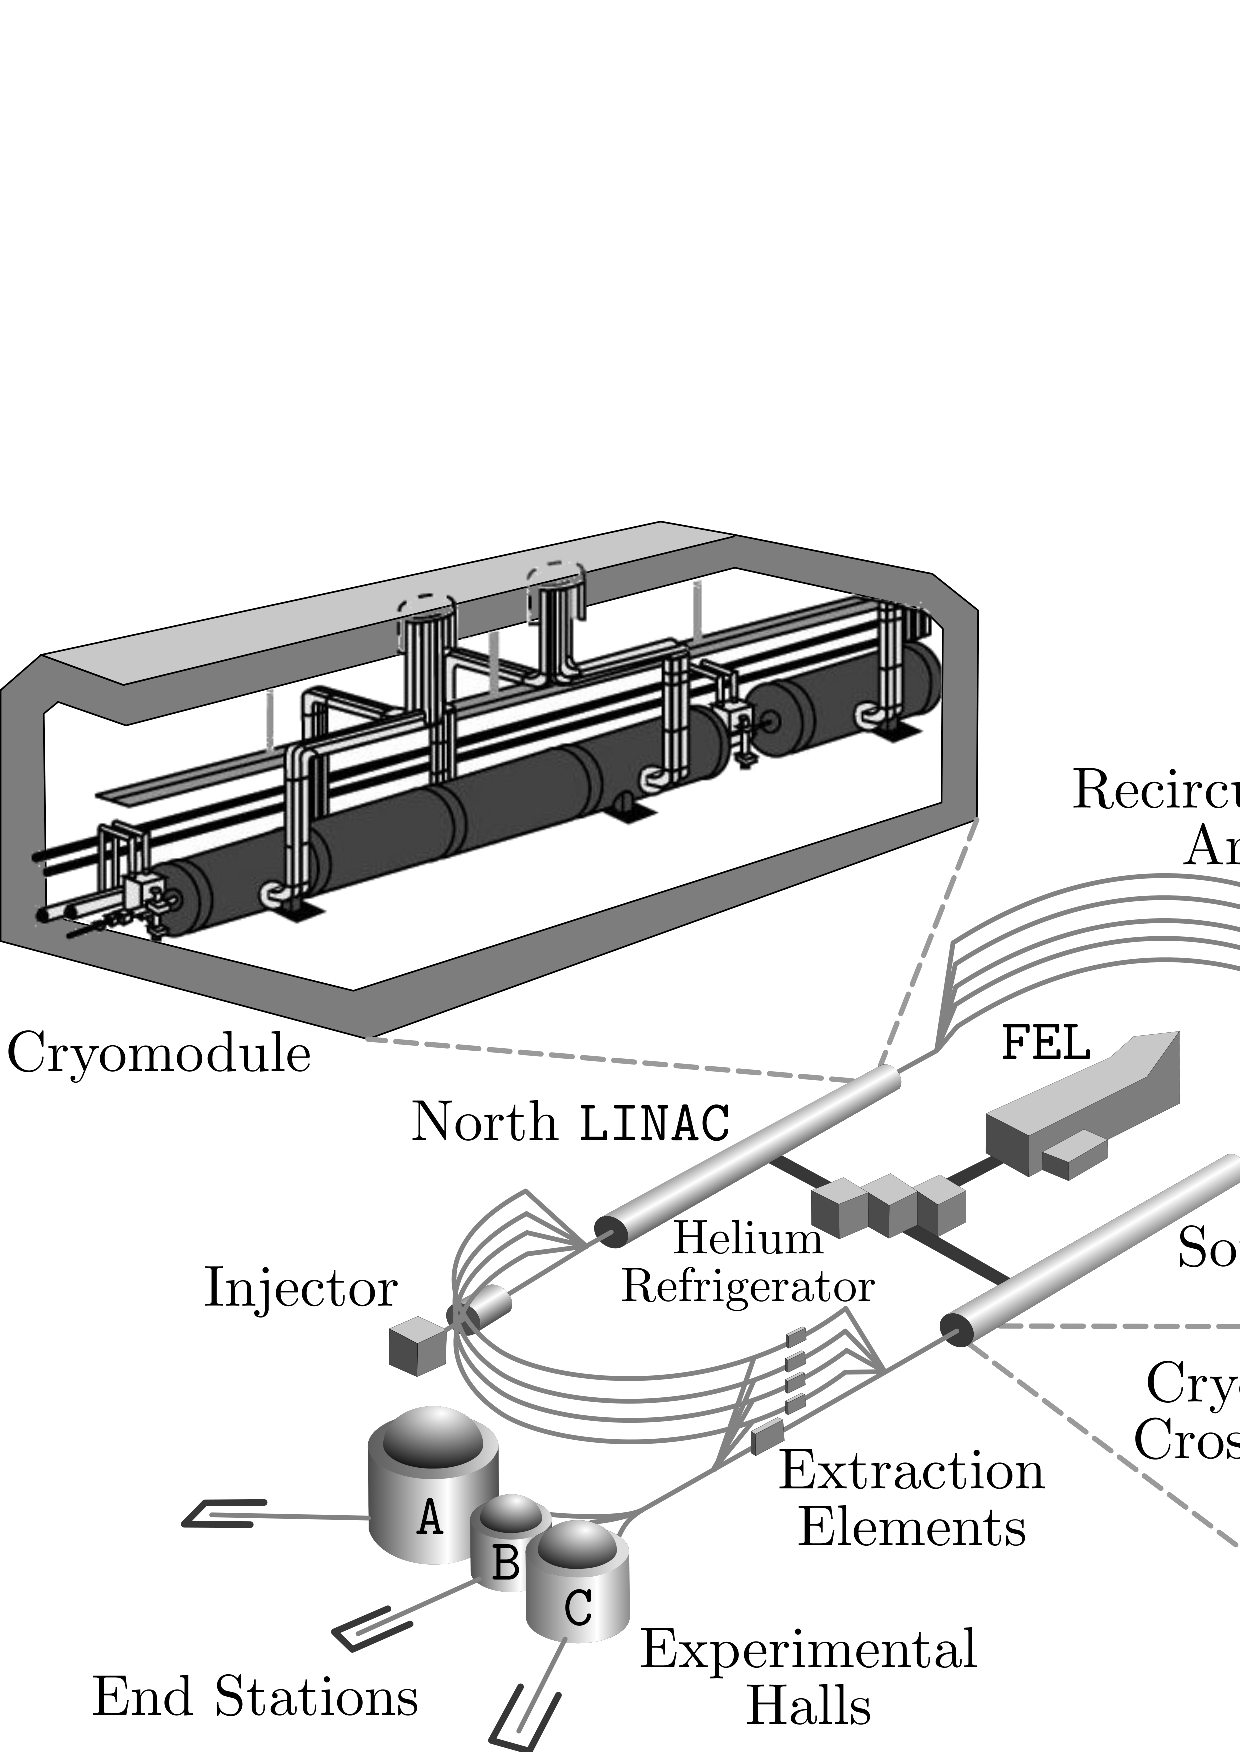
\includegraphics[width=0.9\columnwidth, height=\qfigheight]{\grpath/jlab/cebaf.pdf}
\caption[The Continuous Electron Beam Accelerator Facility (\abbr{CEBAF}) at Jefferson Laboratory (\abbr{JLab})]{\label{fig:jlab.cebaf}The Continuous Electron Beam Accelerator Facility (\abbr{CEBAF}) at Jefferson Laboratory (\abbr{JLab}) showing cross-sections of the linear accelerator (\abbr{LINAC}) halls and the recirculation arcs. Also depicted are the Free Electron Laser (\abbr{FEL}\label{abbr:fel}) and the helium refrigerator and distribution facility. Image Source:\cite{cebaf}}
\end{center}\end{figure}
\FloatBarrier
\section{Continuous Electron Beam Accelerator Facility}\label{sec:cebaf.desc}

\abbr{CEBAF} utilizes superconducting radio-frequency (\abbr{srf}\label{abbr:srf}) cavities to accelerate electrons and provide a continuous wave beam with 75\% polarization to the three halls simultaneously. A list of some specifications for \abbr{CEBAF} can be found in Table~\ref{tab:cebafspecs}.
%Niobium (\abbrlc{N}{b}\label{abbr:nb}), in a cryogenic system, provides the superconducting environment necessary for \abbr{CEBAF} to obtain a 100\% duty factor because superconducting cavities are non-resistive. Prior to the implementation of \abbr{srf}, copper \abbr{RF}\label{abbr:rf} cavities were used, however due to the resistive properties of copper significant cooling time was needed due to heat produced in the cavity.
\begin{table}
\begin{minipage}{\textwidth}
\begin{center}
\begin{singlespacing}

\caption[\abbr{CEBAF} Operating Specifications]{\label{tab:cebafspecs}Operating specifications of \abbr{CEBAF} at \abbr{JLab}.\cite{cebaf}}

\begin{tabular}{c|c}

%\hline \hline
%
%operation & \multicolumn{3}{c}{Generation} \\
%charge & I & II & III \\


\hline

$\textrm{E}_{min}$ & 0.6 GeV \\
$\textrm{E}_{max}$ & 6.0 GeV \\
$\textrm{I}_{max}$ & 200 $\mu$A \\
Polarization & $\textgreater$ 75\% \\
Geometric emittance & $\textless \ 10^{9}$ m rad \\
Momentum Spread & $10^{-5}$ \\
Average currents (Halls A and C) & 1-150$\mu$A \\
Average currents (Hall B) & 1-100nA \\
Bunch charge & $\textless$ pC \\
Repetition rat & 499 MHz/hall \\ 
Beam size (rms transverse) & $\sim$ 80 $\mu$m \\
Bunch length (rms) & 300 fs, 90 $\mu$m \\
Energy spread & 2.5 x 10$^5$ \\
Beam power & $\textless$ \ MW  \\
Beam loss & $\textless \mu$A  \\
Number of passes & 5 \\
Number of accelerating cavities & 338 \\
Fundamental mode frequency & 1947 MHz \\
Accelerating cavity effective length & 0.5m \\
Cells/cavity  & 5\\
Average $Q_{0}$  & 4.0 x 10$^9$ \\
Implemented $Q_{ext}$  & 5.6 x 10$^6$ \\
Cavity impedance (r/Q)  & 980 $\Omega$ \\
Average cavity accelerating gradient  & 7.5 MV/m \\
RF power  & $\textless$ \ 3.5 kW/cavity \\
Amplitude control  & 1.00 x 10$^{-4}$ rms \\
Phase control  & 0.1$^\circ$ rms \\
Cavity operating temperature  &  2.08 K\\
Heat load @ 2 K  &  $\textless$ 9 W/cavity\\
Liquefier 2 k cooling power  & 5kW \\
Liquefier operating power  &  5MW\\




\hline \hline

\end{tabular}

\end{singlespacing}
\end{center}
\end{minipage}
\end{table}
\vspace{20pt} 

To achieve the running conditions described in Table~\ref{tab:cebafspecs} \abbr{CEBAF} uses a GaAs photocathode laser driven injector system to produce a highly polarized electron beam. The laser pulses create three electron bunches that are bunched together in 2 ns groups, about 90 $\mu$m in length. Each bunch is 499~MHz at the source at 100 keV, spaced apart by 120$^\circ$ of \abbr{rf} phase. Together the electron bunches form a 1497 MHz beam that then enters two 1/4 \abbr{srf} cavities which accelerate the electrons to $\sim$1\% of the total machine energy before it is injected into the \abbr{CEBAF}'s main accelerator. 

When the electron bunches enter the \abbrlc{N}{b} \abbr{srf} cavity, they undergo an acceleration gradient provided by \abbr{rf} standing wave established inside of the cavity. The standing waves are kept in phase with the electron bunches resulting in a continuous positive electric force on each bunch as it passed through a cavity, see Fig.~\ref{fig:jlab.accel}

\begin{figure}\begin{center}
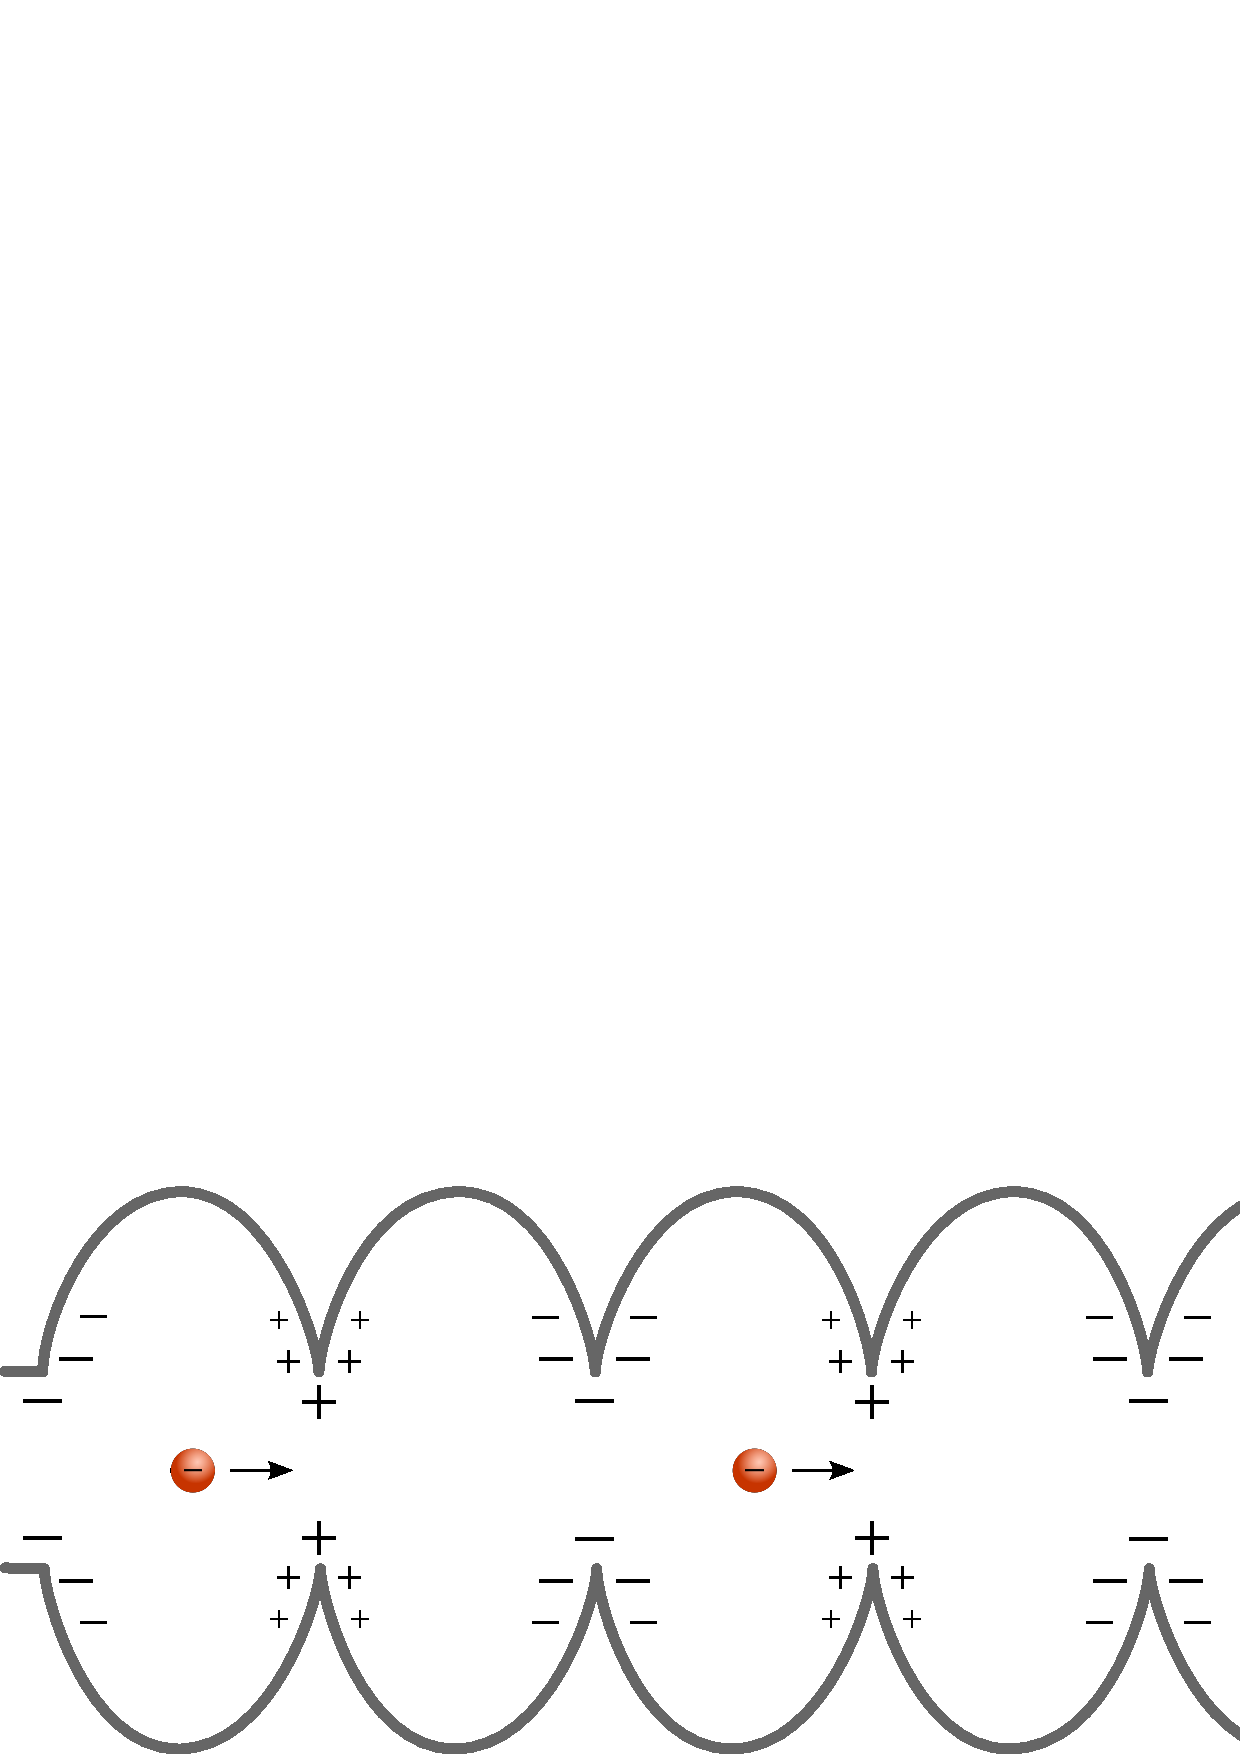
\includegraphics[width=0.8\figwidth,height=\qfigheight]{\grpath/jlab/accelerating_diagram.pdf}
\caption[Accelerating Cavity Diagram]{\label{fig:jlab.accel}Accelerating Cavity Diagram. Electron clusters experience a continuous acceleration due to a standing electromagnetic wave indicated by the positive and negative signs along the inner wall.}
\end{center}\end{figure}

The main accelerator, Fig.~\ref{fig:jlab.cebaf}, consists of a pair of linear accelerators (\abbr{LINAC}s\label{abbr:linac}). Each \abbr{LINAC} contains 168 \abbr{srf} \abbrlc{N}{b} cavities that are submerged in liquid Helium and cooled to 2.08 K, the temperature by which \abbrlc{N}{b} becomes superconducting. In total there are twenty cryogenic modules, each containing eight superconducting niobium cavities as depicted. in Fig.~\ref{fig:jlab.cavity}. 
%The significant cooling requirements are satisfied by the Lab's Central Helium Liquefier (\abbr{CHL}\label{abbr:chl}). 


\begin{figure}\begin{center} 
\includegraphics[width=\figwidth, height=\qfigheight]{\grpath/jlab/niobium_cavity_pair.pdf}
\caption[A \abbr{CEBAF} superconducting niobium cavity pair]{\label{fig:jlab.cavity}A \abbr{CEBAF} superconducting niobium cavity pair. Image Source: \cite{cebaf}}
\end{center}\end{figure}

The beam, once inside the \abbr{LINAC} can be passed up to five times. The \abbr{LINAC}s are connected by two sets of 180$^\circ$ magnetic-dipole bending arcs (see Fig.~\ref{fig:jlab.cebaf}) with a radius of 80~meters. The beam is sent through both accelerators and is then recirculated up to four more times. Each \abbr{LINAC} is capable of accelerating the beam by up to 600~MeV giving approximately 1.2~GeV per pass. Each hall can choose to extract the beam after any number of passes, however the fifth (final) pass can be sent to all three halls simultaneously. It should be noted that although each hall can receive the fifth pass, no two halls can run with the same lower energy \cite{clas.pass}. At the time of the \g12 experiment, the accelerator was capable of delivering a maximum electron beam energy of 5.714~GeV.
%\FloatBarrier
%\FloatBarrier
\section{Circular Polization} \label{sec:clas.polar}

As mentioned in Sec.~\ref{sec:cebaf.desc}, the electron beam provided by \abbr{CEBAF} has the capability of having 75\% longitudinal polarization. Longitudinal polarized electrons produce circularly polarized photons in the bremsstrahlung process on any target, however intensity of photon beam depends on Z of target. The circular polarization production process is quantum mechanical. From QED calculations, the degree of circular polarization transfer to the photon, $P_{circ}$, is seen to depend on the ratio of the relative electron energy to the bremsstrahlung photon, $\epsilon$:
%The experiment \g12 used a Au foil as a radiator therefore \g12 had a circular polarized beam.
\begin{equation}\label{eq:polarization}
	P_{circ} = (\frac{4\epsilon - \epsilon^{2}}{4-4\epsilon+3\epsilon^{2}})P_{e} \cite{Olsen}
\end{equation}
where $\epsilon = k/E_{0}$, $k$ is the bremsstrahlung photon energy and $E_{0}$ is the incident electron energy. Equation~\ref{eq:polarization} shows that circular polarization of the photon is transferred directly from the polarization of the electron, it also shows that the atomic nucleus or radiator plays no role in transfer of polarization. The transfer of circular polarization is maximum at the higher end of the energy spectrum $\epsilon$ and decreases towards the lower end of the spectrum as seen in Fig.~\ref{fig:jlab.polarization}. Figure~\ref{fig:jlab.polarization} also illustrates that polarization transfer is favored when the radiated photons take up large fractions of the incident electron energy. Coulomb and screening corrections (due to the atomic electrons) do not significantly affect the polarization of the emitted photons. 

\begin{figure}[h!]\begin{center}
\includegraphics[width=0.8\figwidth,height=\qfigheight]{\grpath/hall-b/polarization.pdf}
\caption[Circular polarization Graph]{\label{fig:jlab.polarization}QED calculation for the degree of circular polarization of 50-MeV electrons in lead. The curve shown is a Born-approximated calculation which neglects screening corrections. An exact calculation involving Coulomb and screening corrections (not shown) yields similar results.\cite{Olsen}}
\end{center}\end{figure}

\FloatBarrier
\section{Beam Positioning}\label{sec:clas.beam}
%\FloatBarrier
There are several beam monitoring stations in Hall \desg{B} before and after the \abbr{CLAS} detector (Fig.~\ref{fig:clas.beam.beforemonitors}) to scan the important details of the electron beam prior to conversion into a photon beam and the details of the photon beam before and after entering the target. Such quantities for the electron beam include position, intensity, dispersion, and current, and for the photon beam include position, dispersion and flux. Most of these monitoring stations are used by the accelerator group.
% to steer the beam to the target as they control all magnets that can substantially move the beam.
\begin{figure}[h!]\begin{center}
\includegraphics[width=\figwidth, height=1.75\hfigheight]{\grpath/hall-b/beamline_components.pdf}
\caption[Beamline and components of \abbr{CLAS}]{\label{fig:clas.beam.beforemonitors}{\coloronline}Beamline and components of \abbr{CLAS}. Image Source~\cite{cebafflckr}}
\end{center}\end{figure}
There are two types of devices to measure the electron beam position. The first type is represented by two beam position monitors (\abbr{BPM}s\label{abbr:bpm}) placed before the tagger. The position monitors use three radiofrequency cavities to measure the transverse location of the electron beam and its intensity. This information is used as feedback for the steering mechanism. The position monitors are noninvasive and measure at a rate of 1 Hz. 
The second type of device used to measure the beam position is the Harp Beam Profile Monitor, which also measures the electron beam dispersion. The harp devices consist of fine wires (20 and 50~{\um} W and 100~{\um} Fe) that can be passed through the beam at specific orientations and collect scattered electrons with a photomultiplier tube. This procedure measures the horizontal ($x$) and vertical ($y$) profile of the electron beam and is performed after any downtime or change in the beam. The accelerator group adjusts the beam position such that more than 99\% of the electron beam goes through the radiator. Since this process is invasive, it was only done when the drift-chambers and \abbr{DAQ} were turned off. A harp scan measurement for \g12 is shown in Fig.~\ref{fig:clas.beam.harpscan}. The width of the beam was contained within a 200 $\mathrm{\mu}$m diameter.



%\begin{figure}\begin{center}
%\includegraphics[width=\figwidth,height=\hfigheight]{\grpath/hall-b/G12_afterbeam_blueprint.pdf}
%\caption[Beamline and \abbr{CLAS} components in \g12]{\label{fig:clas.beam.aftermonitors}{\coloronline}Beamline and \abbr{CLAS} components in \g12}
%\end{center}\end{figure}

\begin{figure}\begin{center}
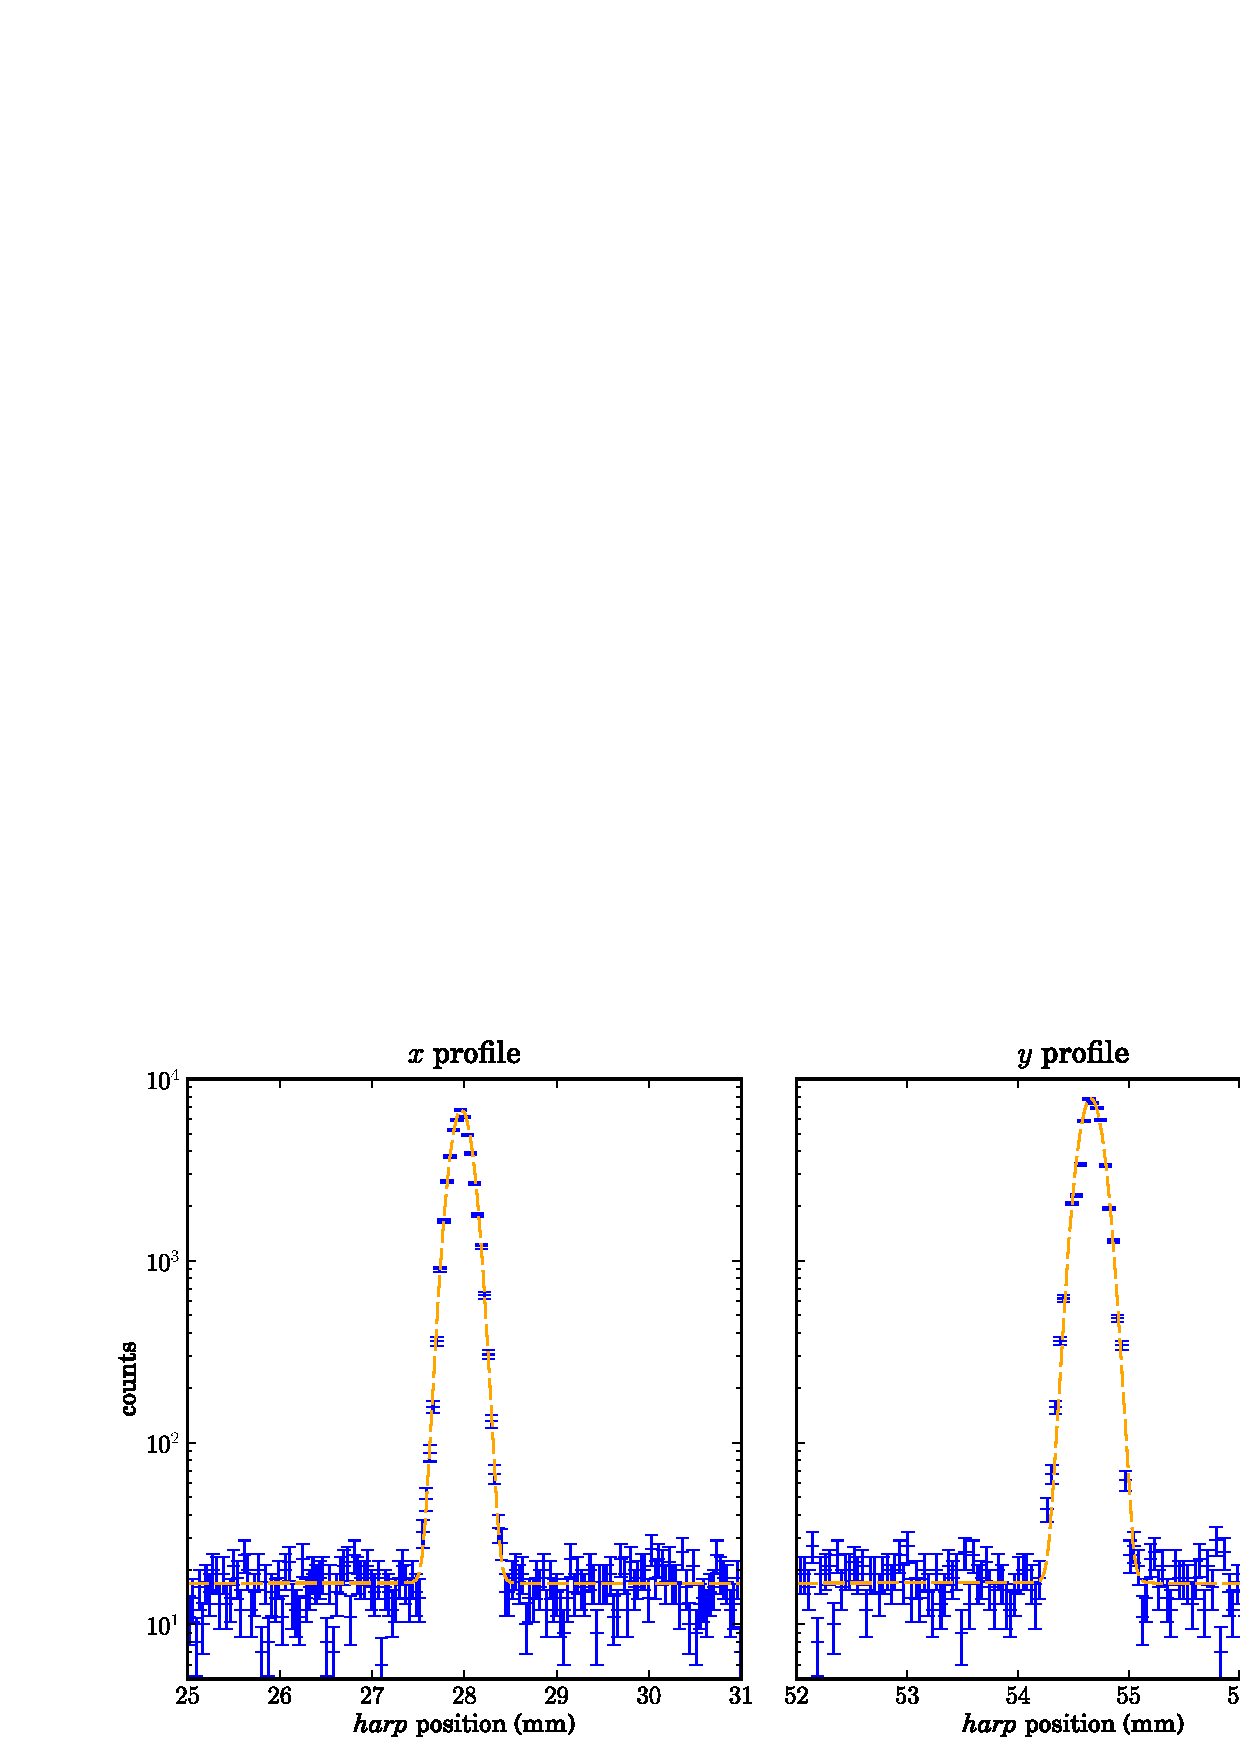
\includegraphics[width=\figwidth,height=\qfigheight]{\grpath/calibration/harpscan.pdf}
\caption[A typical \emph{harp} scan done just prior to run 56426]{\label{fig:clas.beam.harpscan}{\coloronline}A typical \emph{harp} scan done just prior to run 56426. Shown are the $x$ and $y$ profiles of the electron beam just before the tagger. The dashed orange line is a Gaussian fit to the data: $\sigma_x~=~0.115$~mm and $\sigma_y~=~0.105$~mm. Image Source:~\cite{goetz}}
\end{center}\end{figure}

The Total Absorption Shower Counter located downstream of \abbr{CLAS}, measures the photon flux (see Fig.~\ref{fig:clas.beam.afterCLAS}). The \abbr{TASC}, consists of four lead glass blocks of $\sim$ 17 radiation lengths, each coupled to a photo-multiplier tube (\abbr{PMT}\label{abbr:pmt}). The \abbr{TASC} is approximately 100\% efficient at detecting photons at beam currents less than 100~pA\cite{clas.tagger,clas.tagger.calib}. Since \g12 ran with 65~nA current, special low current, 50~pA, normalization runs(see Table~\ref{tab:data.calibruns}) were taken several times throughout \g12. The ratio of electrons detected in the photon tagger (see Sec.~\ref{sec:clas.tagr}) to that of photons detected in the \abbr{TASC} gives the tagging ratio used to calibrate the tagger and measure the flux throughout the entire \g12 run period.
%with hits in the left and right \abbr{TDC} matching in time and a corresponding hit in an E-counter
\begin{figure}[h!]\begin{center}
\includegraphics[width=\figwidth,height=0.8\qfigheight]{\grpath/hall-b/TASC_blueprint.pdf}
\caption[Beamline and components after \abbr{CLAS} ]{\label{fig:clas.beam.afterCLAS}{\coloronline}Beamline components in \g12 after \abbr{CLAS}}
\end{center}\end{figure}

\FloatBarrier
\section{Photon Tagger} \label{sec:clas.tagr}

The electron beam delivered to hall \desg{B} from \abbr{CEBAF} can be sent directly to a target or the electron beam can produce a \emph{real photon} beam by means of bremsstrahlung radiation by passing the electron beam through a radiator. Typical radiators have high atomic number to help reduce contamination of photons produced by electron-electron scattering. The \g12 experiment used a gold (\abbrlc{A}{u}) foil of $10^{-4}$~radiation length. This choice has a double purpose, to maximize the probability of the electron-nucleus interaction given that the bremsstrahlung cross section is proportional to $\mathrm{Z^{2}}$, and to minimize the number of interaction centers such that each electron interacts once, producing only one photon. After the electron beam passes through the radiator, the beam becomes a mixture of photons and electrons that did not interact with the radiator and recoil electrons. The mixed beam then travels into a dipole magnetic field which sweeps the electrons out of the electron-photon beam. The electrons present in the electron-photon beam are directed toward two hodoscope planes, each made of an overlapping array of scintillators to detect the energy-degraded electrons.

%  

The first scintillator plane, referred to as the E-plane (Figs.~\ref{fig:jlab.tagr.energies}, and~\ref{fig:jlab.tagr.paddles}), is used to determine the momentum of the recoiling electrons. The E-plane provides photon energy resolution on the order of 0.1\% of the incident electron beam energy. It consists of 384 paddles that are 20 cm long, 4 mm thick and from 6 to 18 mm wide. The paddles are arranged in an overlapping fashion, thus increasing the number of logical paddles to 767.
The trajectory of an electron or any charged particle in the magnetic field is governed by the equation
\begin{equation}\label{eq:motioninmag}
	p = qrB \ (\mathrm{if}\ \vec{p} \perp \vec{B} )
\end{equation}
where $p$ is the particle's momentum, $q$ is the particle's charge, $r$ is the particle's radius of curvature and $B$ is the magnetic field the particle passes through.
By determining which paddle an electron hit we know the radius of curvature and we can calculate the momentum of the electron. The momentum of the electron can then be used to obtain the energy of the photon by means of the conservation relation 
\begin{equation}\label{eq:tagger.energy}
	E_{\gamma} = E_{0} - E_{e}
\end{equation}
where $E_{0}$ is the energy of the incident electron given by \abbr{CEBAF}, $E_{e}$ is the energy of the recoil electron and $E_{\gamma}$ is the energy of the emitted photon. 

The second scintillator plane, referred to as the T-plane, is used to make accurate timing measurements of the recoiling electrons. This plane comprises of 61 paddles that are each 2 cm thick. The added thickness of these paddles allow for a timing resolution of 110 ps.
% The spectrometer was able to tag photons ranging from 20-95\% of the incident electron beam energy.

The tagger can tag photons of energies from 20 to 95\% of the incident electron beam energy. For \g12 this corresponds to a photon energy range of 1.142 - 5.425~GeV. Due to the high current of the electron beam delivered to \g12 from \abbr{CEBAF} there were usually more than one ``hit'' in the tagger for each event. Normally, the one associated with the photon that caused the event could be obtained by a timing coincidence with the tracks, although there are cases when this photon is ambiguous as discussed in Sec.~\ref{sec:analysis.beam}.

The photons that pass through the radiator then pass through a 6.2~mm diameter collimator. Collimation is used to trim the beam halo prior to arriving at the CLAS cryotarget. In the \g12 experiment the beam entering the cryotraget was 1.5~cm in radius. The collimator was positioned 537~cm upstream of the cryotarget which had a radius of 2~cm. A sweeping magnet were placed after the collimator to remove any charged particles created by interactions of photons with the collimator.

More detailed information on the Hall B tagging system and \abbr{DAQ} of the tagger system can be found in \cite{clas.tagger}.

\begin{figure}\begin{center}
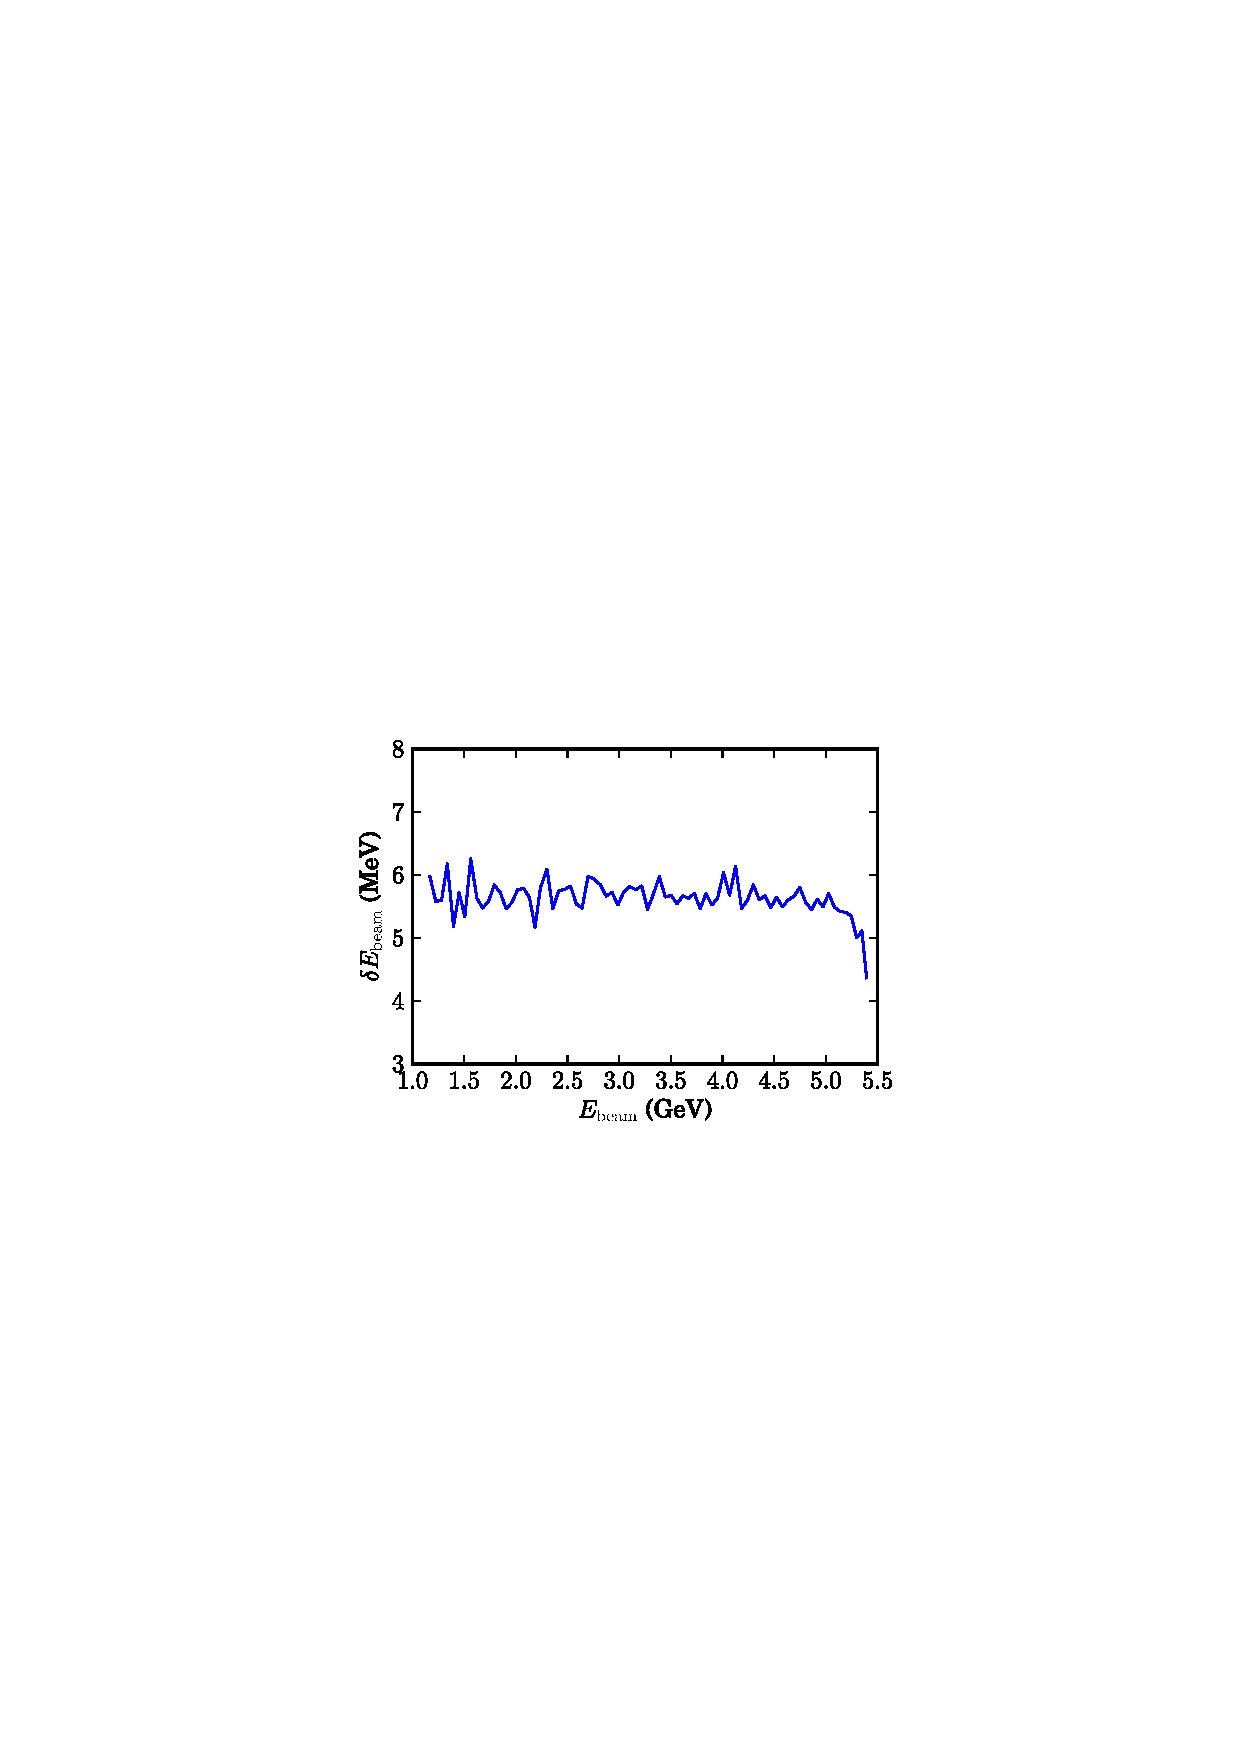
\includegraphics[width=0.8\figwidth,height=\qfigheight]{\grpath/hall-b/tagger_energies.pdf}
\caption[Scale drawing of the photon tagger system]{\label{fig:jlab.tagr.energies}Scale drawing of the photon tagger system. The rectangular area around the $E$ and $T$-counter planes outlines the expanded view shown in Fig.~\ref{fig:jlab.tagr.paddles}.}
\end{center}\end{figure}


\begin{figure}\begin{center}
\includegraphics[width=1.1\figwidth,height=\qfigheight]{\grpath/hall-b/tagger_paddles.pdf}
\caption[Scale drawing of the $E$-counters (blue) and the $T$-counters (green) showing examples of recoiled electrons (red lines) entering from the upper left]{\label{fig:jlab.tagr.paddles}{\coloronline}Scale drawing of the $E$-counters (blue) and the $T$-counters (green) showing examples of recoiled electrons (red lines) entering from the upper left.}
\end{center}\end{figure}
\FloatBarrier

\section{CEBAF Large Acceptance Spectrometer (CLAS)} \label{sec:tjnaf.clas}

The \abbr{CLAS} detector, shown in Figs.~\ref{fig:clas}, ~\ref{fig:clas.ced}, is assembled of four types of detectors, five detectors total,  that are arranged in an onion like pattern (around the beam line) covering $\sim 3\pi$ with a diameter of 8~m. Each layer is segmented such that there are six segments around $\phi$ (angle about the beam line), called sectors, each with a polar coverage, $\theta$ (angle from beam line), of approximately $\frac{3}{4}\pi$~radians. Each sector consists of a scintillator start counter (\abbr{ST}) Sec.~\ref{sec:clas.st}, three layers of drift chambers (\abbr{DC}) Sec.~\ref{sec:clas.dc}, a layer of scintillator ``time-of-flight'' counters (\abbr{TOF}) Sec.~\ref{sec:clas.tof}, a gas Cherenkov counter (\abbr{CC}) Sec.~\ref{sec:clas.cc} and an electromagnetic calorimeter (\abbr{EC}) Sec.~\ref{sec:clas.ec}. There is a toroidal magnetic field generated by six superconducting coils that divide the sectors. The direction of the toroidal field is azimuthal, $\phi$ (angle about the beam line), such that the charged particles conserve their azimuthal angle along their trajectory, except near the coils. The magnetic field geometry guides the particles which allows for a simplified reconstruction algorithm to determine the particles' momenta, see Eq.~\ref{eq:motioninmag}. This section will discuss the subsystems in more detail.
% This field however produces an asymmetry in the acceptance of oppositely charged particles. 


\begin{figure}\begin{center}
\includegraphics[width=0.8\columnwidth,height=0.75 \hfigheight]{\grpath/hall-b/clas_schematic.pdf}
\caption[Schematic of the \abbr{CLAS} detector with subsystems identified]{\label{fig:clas}{\coloronline}Schematic of the \abbr{CLAS} detector\cite{clas} with subsystems identified. This view is looking upstream and the beam enters from the upper left. The detector is approximately 8~meters in diameter.}
\end{center}\end{figure}

\begin{figure}\begin{center}
\includegraphics[width=0.6\columnwidth,height=0.75 \hfigheight]{\grpath/hall-b/clas_D.pdf}
\caption[A cross section view of the \abbr{CLAS} detector showing an event with three tracks emanating from the target]{\label{fig:clas.ced}A cross section view of the \abbr{CLAS} detector showing an event with three tracks emanating from the target. The two tracks leaving hit patterns \abbr{CC} and \abbr{EC} are leptons while the track on the bottom panel is a proton}
\end{center}\end{figure}

\begin{figure}\begin{center}
\includegraphics[width=0.55\columnwidth,height=\qfigheight]{\grpath/hall-b/torus_install.pdf}
\caption[The coils of the \abbr{CLAS} toroidal magnet prior to installation of the rest of the detector]{\label{fig:torusinstall}{\coloronline}The coils of the \abbr{CLAS} toroidal magnet prior to installation of the rest of the detector. Image Source~\cite{williams}}
\end{center}\end{figure}
\FloatBarrier

\subsection{Hydrogen Cryotarget}\label{sec:clas.tgt}


The target used by \g12 was conical as shown in Fig.~\ref{fig:clas.targetblueprint}. The target walls were constructed of 0.127~$\mu$m thick Kapton. It is 40~cm in length and 2~cm in radius. The incident photon beam had a radius of 1.5~cm. The target cell design shown in Figs,~\ref{fig:clas.targetblueprint} and~\ref{fig:clas.targetcell} had been used in several experiments and is capable of containing a number of different materials, such as helium, deuterium and hydrogen. For \g12 the target was filled with liquid hydrogen ($\ell$H$_2$). The temperature and pressure of the target was continuously measured and recorded. In Sec~\ref{sec:analysis.target_density}, these measurements will be used to calculate the density of the liquid Hydrogen to determine the target thickness. The target was not polarized.

\begin{figure}[h!]\begin{center}
\includegraphics[width=\figwidth,height = \qfigheight]{\grpath/hall-b/g11_target_cell_blueprint.pdf}
\caption[Blueprint schematic of the conical Kapton target cell used for \g12]{\label{fig:clas.targetblueprint}Blueprint schematic of the conical Kapton target cell used for \g12.}
\end{center}\end{figure}

\begin{figure}[h!]\begin{center}
\includegraphics[width=0.6\figwidth]{\grpath/hall-b/g11_target_cell.pdf}
\caption[The 40~cm long conical Kapton target cell used for \g12]{\label{fig:clas.targetcell}The 40~cm long conical Kapton target cell used for \g12.}
\end{center}\end{figure}

%\subsubsection{Target Position for \g12}\label{sec:clas.tgt.position}
The target was located 90~cm upstream of \abbr{CLAS} the center, see Fig.~\ref{fig:clas.ced}.
This increased the forward angle acceptance from 8$^\circ$  to 6$^\circ$. However, this also decreased the large angle acceptance from approximately 140$^\circ$ to 100$^\circ$ in the lab frame.
%This reduction in large angle acceptance sacrificed multi-particle final state events, where the final state particles were more than about 70$^\circ$ away from beamline.
%as well as a reduction in \abbr{DC} resolution. The \abbr{DC} resolution decrease was due to the oblique angle the tracks made with the detector planes.
\FloatBarrier
\section{Start Counter}\label{sec:clas.st}

The start counter, Figs.~\ref{fig:clas.st} and~\ref{fig:clas.stxsection}, is a \abbr{PMT}-instrumented scintillator detector that surrounds the CLAS cryotarget hermetically. It consists of 24 scintillation paddles divided into six sectors matching that of \abbr{CLAS}. Each sector of the start counter is constructed of four independently-instrumented scintillator strips. Timing resolution of the start counter is $\sim$350~ps. The start counter information was used the \g12 triggers~\ref{sec.data.trig.lepton}. More information on the CLAS start counter can be found in \cite{clas.st}.

\begin{figure}[h!]\begin{center}
\includegraphics[width=0.8\figwidth,height=\qfigheight]{\grpath/hall-b/start_counter.pdf}
\caption[Schematic of the start counter (\abbr{ST}) with the 40~cm long target cell (purple) at the center]{\label{fig:clas.st}{\coloronline}Schematic of the start counter (\abbr{ST}) with the 40~cm long target cell (purple) at the center. The beam enters from the upper left of the figure.}
\end{center}\end{figure}

\begin{figure}[h!]\begin{center}
\includegraphics[width=0.8\figwidth,height=\qfigheight]{\grpath/hall-b/start_counter_wtarget.pdf}
\caption[Cross-section view of the start counter illustrating the labeled components and its angular coverage when at the center of \abbr{CLAS}]{\label{fig:clas.stxsection}{\coloronline}Cross-section view of the start counter illustrating the labeled components and its angular coverage when at the center of \abbr{CLAS}.}
\end{center}\end{figure}

\FloatBarrier
%\subsection{Start Counter Efficiency Analysis}\label{sec:clas.st.eff}
%There is an inefficiency of the start counter as seen in Fig.~\ref{fig:classt.ineff}. This inefficiency was measured by using real data events as generated events and passing them through \abbr{CLAS}'s Monete-Carlo package(\abbr{GSIM}\label{abbr:gsim}). More information about this inefficiency will be discussed in Sec.~\ref{sec:analysis.accept.verify}.
%
%%It was observed that 20~\% of the events would fail in simulation, this will be discussed in Sec~\ref{sec:gsim.efficiency}. A portion of the failed events were based upon a failure to reconstruct the required banks for the start counter. This phenomena was investigated from the raw data and found to also be present in the processing of the data from raw to user file in the same manner as seen from Monte-Carlo. The blue-dashed line in Fig.~\ref{fig:classt.ineff} illustrates the start counter inefficiency that is dependent on the events reconstructed vertex. The inefficiency is due to the start counter reconstruction algorithm not being able to link the start counter hit to a track through time-based tracking. This track is not lost due to a reprocess of time-based tracking, linking the track to another particles start counter hit with the same 
%
%%The inefficiency of the start counter is not a mechanical fault but rather the fault of the algorithm used to reconstruct a start counter hit. TO study this raw data events were processed event by event using the program DDD and \abbr{CLAS} event display (\abbr{ced}). Unknown of the cause, it  
%
%
%\begin{figure}[h!]\begin{center}
%\includegraphics[width=0.8\figwidth,height=0.7\hfigheight]{\grpath/hall-b/st_issue_4_thesis.pdf}
%\caption[Start Counter Inefficiency]{\label{fig:classt.ineff}{\coloronline}Plot showing the inefficiency of the start counter from data events, red-solid line is the inefficiency of reconstruction based solely on hit-based tracking, blue-dashed line is inefficiency of start counter, black-solid is combined. }
%\end{center}\end{figure}
%
%\FloatBarrier
\section{Superconducting Toroidal Magnet}\label{sec:clas.tor}

The essence of \abbr{CLAS} is the use of a toroidal magnetic field generated by six superconducting coils consisting of 4 layers of 54 windings of aluminum-stabilized niobium titanium NbTi/Cu superconductor \cite{clas}. The coils are separated in the azimuthal direction, $\phi$, by 60$^\circ$ and are located between Region-1 and Region-3 of the \abbr{DC}, see Fig~\ref{fig:clas.dc.torus.mag}. The placement of the coils is such that the magnetic field is encompassed by the volume of the \abbr{DC}, see Fig.~\ref{fig:clas.dc.torus.mag}. The direction of the toroidal field points along $\phi$, except near the coils,  such that the charged particles conserve their azimuthal angle along their trajectory, see Fig~\ref{fig:clas.dc.torus.cont}. The maximum current the magnet can support is 3861~A, resulting in a maximum field strength of 35~kG. During the \g12 experiment, the magnets operated at a current of 1930~A corresponding to a maximum field of about 20~kG. The field was oriented such that positive charged particles bent away from the beam-line, while negative charged particles bent toward the beam-line. Running at higher currents provides better momentum resolution but decreases the detector's acceptance for negative particles. Knowing the strength and direction of the magnetic field and the trajectory of a particle using the \abbr{DC}, the particle momentum can be determined by use of Eq.~\ref{eq:motioninmag}.
% During the \g12 experiment, the magnet was cooled down to 4.5~K using liquid helium ($\ell$He) obtained from the central CEBAF central cryogenic facility.

\begin{figure}[h!]\begin{center}
\includegraphics[width=\figwidth,height=0.9\qfigheight]{\figures/hall-b/torus_field_mag_mount.pdf}
\caption[The \abbr{CLAS} Superconducting Toroidal Magnet and its placement in relation to Region-1 and Region-3]{\label{fig:clas.dc.torus.mag}The \abbr{CLAS} Superconducting Toroidal Magnet and its placement in relation to Region-1 and Region-3  (left). Cross-section of the \abbr{CLAS} Superconducting Toroidal Magnet at half current (1930~A). Region-2 of the \abbr{DC} is located inside the region of the coils shown as the kidney shaped loop at about 3~kG (right).}
\end{center}\end{figure}

\begin{figure}[h!]\begin{center}
\includegraphics[width=1.\figwidth,height=0.75\hfigheight]{\figures/hall-b/torus_field_and_DC.pdf}
\caption[Schematic cross-sectional view of the \abbr{CLAS} detector, perpendicular to the beam line]{\label{fig:clas.dc.torus.cont}Schematic cross-sectional view of the \abbr{CLAS} detector, perpendicular to the beam line (left). The magnetic field distribution corresponding to the view in the left figure. The field is purely azimuthal. The six torus coils are shown in grey, the field is in the counter-clockwise direction,  the field strength is concentrated in the region between the coils (right).}
\end{center}\end{figure}

\FloatBarrier
\section{Drift Chambers}\label{sec:clas.dc}

The \abbr{CLAS} drift chambers \abbr{DC} (Figs.~\ref{fig:clas},~\ref{fig:clas.dc.torus.cont},~\ref{fig:clas.dc.drift}) track charged particles above 200~MeV/c with polar angle resolution of 2-4~mrad and momentum resolution of 0.5 - 1\%, depending on momentum, see Fig~\ref{fig:clas.dc.res}. Typical coverage of the \abbr{DC} is $8^\circ < \theta < 142^\circ$, when the target is at \abbr{CLAS} center. For the \g12 experiment the coverage of the \abbr{DC} was modified to $6^\circ < \theta < 100^\circ$ due to the placement of the target, see Sec~\ref{sec:clas.tgt} for reasons explained in ~\cite{clas.proposal.hyclas},~\cite{clas.proposal.superg},~\cite{clas.proposal.pion}.
\begin{figure}\begin{center}
\includegraphics[width=0.8\figwidth,height=0.75\hfigheight]{\figures/hall-b/drift_DC_resolution.pdf}
\caption[Momentum and angular resolution for protons as determined from the measured angle of the scattered electron for data collected and Monte-Carlo simulation]{\label{fig:clas.dc.res}Momentum and angular resolution for protons as determined from the measured angle of the scattered electron for data collected and Monte-Carlo simulation. Image Source~\cite{clas}}
\end{center}\end{figure}

The \abbr{DC} are divided into six sectors each containing three radial layers (Fig.~\ref{fig:clas.dc.drift}), referred to as ``Regions'', for a total of 18 separate drift chambers. Each \abbr{DC} region covers the same polar angular range and consist of two superlayers which each contain six layers of hexagonal wire cells which house evenly spaced 20~$\mu$m gold-plated tungsten sense wires (center of hexagon) each surrounded by six 140~$\mu$m gold-plated aluminum alloy field wires (vertices of hexagon). In the first superlayer, the wires are strung approximately parallel to the direction of the magnetic field (axial wires), while the second superlayer has wires tilted at a 6$^\circ$ angle with respect to the axial wires (stereo wires). A high voltage system maintains the sense wires at positive potential, while the field wires are maintained at a negative potential 50\% lower than the positive value. The difference of potentials creates an avalanche of the electrons induced by the ionizing particle. The hexagonal shape of the cell mimics a circular geometry cell in which the drift time to drift distance is independent of entrance angle.

The inner region is denoted as Region 1. Its first superlayer has only 4 layers due to space constraints. Region 1 is nearly free from magnetic field, see Fig~\ref{fig:clas.dc.torus.mag}. Region 2 is situated between the magnetic coils which is subject to the highest magnetic field which is used to determine the particle's curvature, needed to determine the particle;s momenta, see Eq.~\ref{eq:motioninmag}. Region 3 purpose is to provide global track reconstruction in connection with other CLAS detectors since Region 3 is located outside the volume of magnetic field. Each \abbr{DC} is filled with a gas mixture of 90\% argon and 10\% carbon-dioxide. This choice of gas provides high drift velocity (0.04 m/$\mu$sec) and fast collection time which improves momentum resolution. For more information on the design of the \abbr{CLAS} \abbr{DC} system, see~\cite{clas.dc} and for more information on the calibration process of the \abbr{CLAS} \abbr{DC} system, see~\cite{clas.dc.calib}.

\begin{figure}\begin{center}
\includegraphics[width=\figwidth,height=0.75\hfigheight]{\figures/hall-b/drift_DC_cedII.pdf}
\caption[A cross section view of the \abbr{CLAS} detector showing an event with three tracks emanating from the target]{\label{fig:clas.dc.drift}A cross section view of the \abbr{CLAS} detector showing an event with three tracks emanating from the target. The two tracks leaving hit patterns \abbr{CC} and \abbr{EC} are leptons while the track on the bottom panel is a proton. The inlet shows hexagonal cells of drift chambers with a typical track indicated by shaded areas for the cut-out in Region-3.}
\end{center}\end{figure}

\FloatBarrier
\section{Cherenkov Radiation and Detectors}\label{sec:clas.cc}

When a charged particle traverses through a medium with a velocity less than the speed of light for that medium ($v < c/n$) the dipoles of the molecules in the medium are symmetrically arranged such that the integrated dipole field along the particles path vanishes. However, when the particles speed is greater than that of the speed of light for that medium the dipoles of the molecules arrange themselves such that they are asymmetric along the particles path and thus creates a dipole field, see Fig~\ref{fig:clas.cc.dipole}.
\begin{figure}[h!]\begin{center}
\includegraphics[width=\figwidth,height=\qfigheight]{\figures/hall-b/CCECPLOTS/cherenkov.pdf}
\caption[Illustration of Cherenkov Radiation]{\label{fig:clas.cc.dipole}Illustration of Cherenkov Radiation. Negative charged particle traveling through a medium with $v < c/n$ showing dipoles symmetrically arranged around particles path (left). Negative charged particle traveling through a medium with $v > c/n$ showing dipoles asymmetrically arranged around particles path given rise to dipole field(right). Image Source:~\cite{cherenkov_image}}
\end{center}\end{figure}

The generated dipole field radiates the energy contained in this disturbance producing a coherent shockwave, this is known as Cherenkov radiation. An analogy of this phenomena is the sonic boom created in air from an object traveling faster then the speed of sound. Just as the sound wave of a sonic boom travels slower than the traveling object, so does the light emitted from the dipole field. This reduction in velocity creates the wave front of a continuous light spectrum, see Fig~\ref{fig:clas.cc.angle}.
\begin{figure}[h!]\begin{center}
\includegraphics[width=\figwidth,height=0.75\hfigheight]{\figures/hall-b/CCECPLOTS/cc_wavefront_madeII.pdf}
\caption[Illustration of Cherenkov Angle]{\label{fig:clas.cc.angle}Illustration of Cherenkov Angle. When the particle has traveled the distance $\mathrm{RP =\nu t \rightarrow \beta c t}$, the photon (light front) has traveled $(c/n)t$.}
\end{center}\end{figure}

Inspecting Fig~\ref{fig:clas.cc.angle}, when the particle has traveled the distance $\mathrm{RP =\nu t = t \beta c}$, the photon has traveled $(c/n)t$, therefore
\begin{equation}\label{eq:cherenkov_eq}
 \mathrm{\cos\theta_{c} = \frac{(c/n)t}{t \beta c} = \frac{1}{n\beta}}
\end{equation}
and the threshold of Cherenkov radiation is 
\begin{equation}\label{eq:cherenkov_threshold}
 \mathrm{\beta_{th} > \frac{1}{n}}.
\end{equation}
Adding in quantum effects
\begin{equation}\label{eq:cherenkov_eq_quantum}
\mathrm{cos\theta_{c} = \frac{1}{n\beta} + \frac{\Lambda}{\lambda}\frac{n^{2} -1}{2n^{2}}}
\end{equation}
where
\begin{equation}\label{eq:cherenkov_eq_quantum_lambda}
\mathrm{\Lambda = \frac{\sqrt{1-\beta^{2}}}{\beta}\lambda_{0}} \ , 
\end{equation}
$\mathrm{\lambda =}$ wavelength of light in medium, and $\mathrm{\lambda_{0} }$ is the Compton wavelength 0.024 \AA. For practical cases, and using \abbr{CLAS}, the 2$^{nd}$ order term is negligible (n=1.00153). To illustrate that quantum effects are negligible, an electron traveling at threshold in \abbr{CLAS} \abbr{CC},
\begin{equation}
\mathrm{\beta_{th} > \frac{1}{n}} > 0.998472,
\end{equation}

\begin{equation}
\mathrm{\frac{\Lambda}{\lambda}\frac{n^{2} -1}{2n^{2}} =  1.07874 \cdot 10^{-9}}
\end{equation}
%

In \abbr{CLAS}, the Cherenkov counter (\abbr{CC}) is used to detect electrons and positrons while rejecting pions for momenta less than 2.5~GeV. The gas used in the \abbr{CC} for \g12 is perfluorobutane (C$_4$F$_{10}$) with an index of refraction of 1.00153. The threshold energy for producing Cherenkov radiation in C$_4$F$_{10}$ is
\begin{align}
\mathrm{E_{th} = \gamma_{th} m_{0}} \mathrm{ \ (Units \ of \ c)} \\
\mathrm{\gamma_{th} = \frac{n}{\sqrt{n^{2} -1}}} = 18.09
\end{align}
therefore the threshold energy of e$^{\pm}$ is 9.23~MeV while the threshold energy of $\pi^{\pm}$ is 2.52~GeV.
%
The number of photons emitted per unit length at threshold for electrons or positrons is;
\begin{align}\label{eq:cc.NPE}
\frac{dN}{dx} = 2\pi z^2 \alpha \frac{\sin \theta_{c}^2}{\lambda^2} d\lambda = 0.241246 \frac{d\lambda}{\lambda^2}
\end{align}
where $\alpha$ is the fine structure constant, $z =1$ for electrons and positrons, and $\lambda$ is the wavelength at which the photon is emitted. Table~\ref{tab:cc_npe} lists the number of photons/cm for various wavelengths of light for the midpoint of $\beta_{th}$ and a maximum velocity $\beta =1$. Table~\ref{tab:cc_npe} also lists the mirror reflectivity for that wavelength.
\input{tables/cc_nphotons}

The \abbr{CC} subsystem is physically located in the space between Region 3 of the \abbr{DC} subsystem and the \abbr{TOF} in the forward region covering polar angles 8$^\circ$ to 45$^\circ$ in each sector when the target is at \abbr{CLAS} center. For \g12 since the target was placed 90~cm upstream, the polar coverage was approximately from 6$^\circ$ to 35$^\circ$ in the lab frame. The \abbr{CLAS} \abbr{CC}'s were fabricated as 6 independent identical sectors, with each sector divided into 18 regions of $\mathrm{\theta}$, and each $\mathrm{\theta}$ segment divided into 2 modules. Light from Cherenkov radiation is focused in $\mathrm{\phi}$ thus preserving information on the lepton polar angle $\theta$. The optical element of \abbr{CC} module comprises an assembly of one elliptical and one hyperbolic mirror providing primary light focusing into a  ``Winston" light collection cone, a  cylindrical mirror used to compensate for imperfections in the focusing, and a photomultiplier used to count the  number of photons in the light cone, see Fig~\ref{fig:clas.cc_array}. More information on the \abbr{CLAS} Cherenkov detector can be found in~\cite{clas.cc} 

The use of the \abbr{CC} was not included in the original proposals, however a significant drop in price on C$_4$F$_{10}$ just prior to the start of \g12 allowed the gas to be added at the last minute. The price drop was due to the recent availability of another, much cheaper gas that was demonstrated to have the same general properties as C$_4$F$_{10}$ and when \g12 contacted the original supplier of the C$_4$F$_{10}$ for a price match, they committed. 

\begin{figure}[h!]\begin{center}
\subfloat[]{
\includegraphics[width=\figwidth,height=0.5\hfigheight]{\figures/hall-b/CCECPLOTS/CCarray}\label{fig:clas.cc_array}
}\\
%[Schematic of one \abbr{CC} showing the 18 symmetrical, mirrored segments of the CLAS \abbr{CC}]
\subfloat[]{
\includegraphics[width=0.9\columnwidth]{\figures/hall-b/cc_diagram.pdf}\label{fig:clas.cc}
}
\caption[Schematic of one \abbr{CC} showing the 18 symmetrical, mirrored segments of the CLAS \abbr{CC}]{Schematic of one \abbr{CC} showing the 18 symmetrical, mirrored segments of the CLAS \abbr{CC}~(a). Diagram of one segment of the Cherenkov counters with an electron entering from the bottom~(b).}

\end{center}\end{figure}






\FloatBarrier
\section{Time-of-Flight Detectors}\label{sec:clas.tof}

The \abbr{CLAS} time-of-flight \abbr{TOF} subsystem provides precise timing measurements of charged particles that transverse the \abbr{CLAS} detector to help determine the particle masses. The \abbr{TOF} subsystem was also used in the \g12 level 1 trigger (see Sec.~\ref{sec:data.trig}) to identify track candidates. The \abbr{TOF} is constructed of organic plastic scintillant (Bicron BC-408). Scintillation is a process undergone by material when radiation traverses a medium.
%
% At room temperature, all valence electrons of the scintillating material are in the $\mathrm{S_{0}}$ ground state. As a particle propagates through the material the incident radiation populates $\mathrm{S_{1}}$ states. Vibrational levels within $\mathrm{S_{1}}$ band decay radiation-less to $\mathrm{S_{1}}$  base states, which in turn decays under emission of light to the $\mathrm{S_{0}}$ band. The radiation-less decay from the excited $\mathrm{S_{1}}$ band to the ground $\mathrm{S_{1}}$ band is known as internal degradation and is responsible for the transparency of the scintillators to their own radiation. $\mathrm{S_{1}}$ can also decay to adjacent triplet levels however, this decay is highly forbidden by multipole selection rules. If this decay does occur, the decay energy is lower causing the decay time to be longer, see Fig.~\ref{fig:clas.scint_bands} for the illustration of this process. Depending on the properties of the scintillator, decay of fluorescent state in organic plastic scintillators have a typical time between 1-3~ns
%
%%\begin{figure}[h!]\begin{center}
%%\includegraphics[width=\figwidth,height=0.5\hfigheight]{\figures/hall-b/CCECPLOTS/Calorimetry/scint.pdf}\label{fig:clas.scint_bands}\caption[Typical Energy Levels of scintillating material ]{Diagram of scintillating population of states. Image Source~\cite{vibe_levels}}
%%\end{center}\end{figure}
%\begin{figure}[h!]\begin{center}
%\includegraphics[width=\figwidth,height=0.5\hfigheight]{\figures/hall-b/CCECPLOTS/Calorimetry/scint.pdf}
%\caption[Typical Energy Levels of scintillating material ]{\label{fig:clas.scint_bands}Diagram of scintillating population of states. Image Source~\cite{vibe_levels}}
%\end{center}\end{figure}

The \abbr{TOF} subsystem is located between the \abbr{CC} and \abbr{EC} subsystems approximately 4~m from \abbr{CLAS} center, 5~m from the \g12 target. Each sector 57 scintillator paddles divided into two subgroups. The first subgroup subtends angles of 8.6$^\circ$ to 45.9$^\circ$ and consists of 23 scintillating paddles that are 15~cm in width. Each paddle is instrumented with two 2-in diameter \abbr{PMT}'s, see Fig~\ref{fig:clas.tof.paddles}. The first group was optimized for timing resolution while being cost-effective and covering a large area. The second group consists of 34 paddles that are 22~cm wide, covering polar angles from 45.9$^\circ$ to 142$^\circ$. Each paddle in this range is instrumented with two 3-in diameter \abbr{PMT}'s. All paddle bars are 5.08~cm thick for 100\% detection of minimum-ionizing tracks and a timing resolution of 150--200~ps.
%These forward angle counters \abbr{PMT}'s have a 15.9~cm$^2$ photocathode area which covers the 76.2~cm$^2$ cross-sectional area of the scintillator.
%These large angle counter \abbr{PMT}'s have a 30.2~cm$^2$ photocathode area which covers the 118.8~cm$^{\mathrm{2}}$ cross-sectional area of the scintillator.
\abbr{TOF} information is used to reconstruct a particle's mass is by measuring the difference between the event RF corrected start time and the time measured by the \abbr{TOF}, $t_{stsc}$. The RF corrected start time is the radio-frequency time (RF) from the accelerator beam aligned withe the event start time. Using this time, $t_{stsc}$, the length of trajectory to the \abbr{TOF}, $l_{stsc}$, and the speed of light $c$, the particles' velocity can be calculated as
\begin{equation}\label{eq:beta.cal}
\beta = l_{sc}/(t_{c}\cdot c)
\end{equation}
The particle's mass can be reconstructed from the measured velocity and momentum:
%Once the particles velocity is determined as well as the momentum, from the \abbr{DC} subsystem,  the particle mass can be reconstructed as 
\begin{equation}\label{eq:mass.cal}
m = p\sqrt{(1-\beta^2)}/\beta
\end{equation}

\begin{figure}\begin{center}
\includegraphics[width=\figwidth]{\figures/hall-b/tof_paddlesII.pdf}
\caption[Diagram of one sector of the time-of-flight (\abbr{TOF}) paddles]{\label{fig:clas.tof.paddles}Diagram of one sector of the time-of-flight (\abbr{TOF}) paddles. There are 57 scintillator paddles covering the entire acceptance region of the drift-chambers for each sector. \abbr{PMT}'s are outlined in red while a scintillator paddle is outlined in yellow.  Image Source:~\cite{clas.tof}}
\end{center}\end{figure}

\FloatBarrier
%\begin{figure}\begin{center}
%\includegraphics[width=\figwidth]{\figures/hall-b/tof_paddles.pdf}
%\caption[Time-of-Flight Paddles]{\label{fig:clas.tof.paddles}Diagram of one sector of the time-of-flight (\abbr{TOF}) paddles. There are 57 scintillator paddles covering the entire acceptance region of the drift-chambers for each sector.}
%\end{center}\end{figure}
%
%\begin{figure}\begin{center}
%\includegraphics[width=0.8\columnwidth]{\figures/hall-b/clas_detector.pdf}
%\caption[\abbr{CLAS} Detector (photograph)]{\label{fig:clas.photo}The \abbr{CLAS} detector during a maintenance period where the time-of-flight ``shell'' (left) was pulled back from the drift-chambers (\abbr{DC}, right). The beam line enters from the lower right on the other side of the \abbr{DC}. The \abbr{TOF} paddles seen are the two center \emph{panels} shown in Fig.~\ref{fig:clas.tof.paddles} for three of the \abbr{CLAS} sectors.}
%\end{center}\end{figure}
%
%\begin{figure}\begin{center}
%\includegraphics[width=\figwidth]{\figures/reconstruction/coverage_tof.pdf}
%\caption[Time-of-Flight Angular Coverage]{\label{fig:clas.tof.coverage}{\coloronline}Angular coverage in the lab frame of the tracks that had an associated time-of-flight hit. This can be interpreted as the total drift-chamber coverage of the \abbr{CLAS} detector.}
%\end{center}\end{figure}

\section{Electromagnetic Calorimeters}\label{sec:clas.ec}

The calorimetric method implies total absorption of the particle energy in a bulk of material followed by the measurement of the deposited energy. The process usually involves several layers of absorbers and detectors. Depending on the energies and species of particles there are different types of calorimeters. For instance, a 10~GeV muon will require 9~m of Fe or 8~m of Pb to absorb all the energy of the muon. However, a 10~GeV electron will only require 0.2~m of Pb to absorb all the energy.The Electromagnetic Calorimeter was built and used for detection of neutral particles as well as discrimination between electrons and pions.

%\begin{figure}[h!]\begin{center}
%\includegraphics[width=\figwidth,height=\qfigheight]{\figures/hall-b/CCECPLOTS/Calorimetry/detectors.pdf}
%\caption[Types of Calorimeters]{\label{fig:clas.ec.calorim}Type of calorimeter depends on type of hadron detection Image Source:~\cite{C5}}
%\end{center}\end{figure}

\subsection{Electromagnetic Calorimeter}

At energies greater than 100~MeV, electrons lose their energy predominantly by bremsstrahlung while photons lose their energy by electron-positron pair production. The process of bremsstrahlung is electromagnetic radiation produced by the deceleration of an electron when deflected by an atomic nucleus i.e. $\mathrm{e Z \rightarrow Ze\gamma}$. Its cross-section is proportional to $\mathrm{Z^{2}}$ of the material the electron propagates through. The radiation loss of electrons with initial energy $E_0$ can be described as
\begin{align}\label{eq:electron_eloss}
-(\frac{dE}{dx})_{rad} = \frac{E}{X_{0}} \\ \vspace*{10 mm} E(x)=E_{0}e^{\frac{-x}{X_{0}}} 
\end{align}
where $X_{0}$ is the radiation length of the material the electron travels through. The process of pair production, $\gamma Z \rightarrow Ze^{+}e^{-}$ was discussed in Sec.~\ref{sec:intro.conversion}.
%, occurs when a photon with $E_0 > 2 m_e c^2$ converts into an electron and a positron. The cross section for this process can be simplified as
%\begin{equation}\label{pair_crosssection}
%\sigma_{\gamma\rightarrow e^+e^-} =  \frac{A}{N_{A} \rho \lambda_\gamma}  \ ,\ \lambda_\gamma = \frac{9}{7}X_0
%\end{equation}
%where $\lambda$ is also know as the interaction length, or mean free path, $\rho$ is the density of the material, $N_A$ is Avogadro's number and $A$ being the atomic mass of the material. The probability of pair production to occur is solely based on $X_{0}$, the radiation length of the medium and this probability can be expressed as
%\begin{equation}
%\frac{dP}{dx} = \frac{1}{\lambda_\gamma}\exp(\frac{-x}{\lambda_\gamma}) \ .
%\end{equation}

To explain how an Electromagnetic Calorimeter works, assume the absorber for the calorimeter is lead(Pb), Fig \ref{fig:clas.photon_processes} , \ref{fig:clas.electron_processes} depicts the processes for photons and electrons in Pb.
\begin{figure}[h!]\begin{center}
\subfloat[][]{
\includegraphics[width=0.45\columnwidth,height=0.5\hfigheight]{\figures/hall-b/CCECPLOTS/Calorimetry/PhotonRadiations.pdf}\label{fig:clas.photon_processes}
}
\subfloat[][]{
\includegraphics[width=0.45\columnwidth,height=0.5\hfigheight]{\figures/hall-b/CCECPLOTS/Calorimetry/EectronE2.pdf}\label{fig:clas.electron_processes}}
\caption[Photon and Electron processes in \abbr{Pb}]{Photon and Electron processes in \abbr{Pb}~(a) and (b) respectively. Images Source:~\cite{vibe_levels}} 

\end{center}\end{figure}
Lets start with a high energy electron $E_{0}$, after $1 X_{0}$, $\mathrm{1e^{-}}$ and $\mathrm{1 \gamma}$ are produced each with $\frac{E_{0}}{2}$, after $2 X_{0}$, $\mathrm{2e^{-}}$, $\mathrm{1e^{+}}$ and $\mathrm{1 \gamma}$ are produced each with $\frac{E_{0}}{4}$. Therefore after $tX_{0}$, there is a total of 
\begin{equation}
N(t)=2^{t}
\end{equation}
are produced each with
\begin{equation}
E(t) = E_{0}2^{-t}.
\end{equation}
The multiplication of the shower particles continue as long as
\begin{equation}
\frac{E_{0}}{N} > E_{c},
\end{equation}
where $E_{c}$ is the critical energy for showers to propagate,
\begin{align}
E_{c}  = E_{0}2^{-t_{max}} \\
N_{max}=\frac{E_{0}}{E_{c}}
\end{align}

\begin{figure}[h!]\begin{center}
\includegraphics[width=\figwidth,height=\qfigheight]{\figures/hall-b/CCECPLOTS/Calorimetry/cascade.pdf}
\caption[A simple Electromagnetic shower in a calorimeter]{\label{fig:clas.ec.shower}{A simple Electromagnetic shower in a calorimeter} Image Source:~\cite{vibe_levels} }
\end{center}\end{figure}

When a particle falls below critical energy, absorption processes (ionization, Compton and photoelectric) start to dominate the processes for photons and electrons. This leads to
\begin{equation}
t_{max} = \frac{ln(\frac{E_{0}}{E_{c}})}{ln2}.
\end{equation}
At the shower maximum $\mathrm{e^{\pm}}$ will stop within $1X_{0}$ however, photons at critical energy will penetrate further. To absorb 95\% of photons produced in the shower maximum, an additional 7-9$X_{0}$ is necessary. The semi-empirical value for $\mathrm{e^{\pm}}$ $E_c$ in Pb is,
\begin{equation}
E_{c}  \thickapprox \frac{610 MeV}{\mathrm{Z} - 1.24} = 7 MeV 
\end{equation}
which results in $t_{max} \thickapprox 9.7 X_{0}$ for electrons at 6 GeV.

The process shown in Fig~\ref{fig:clas.ec.shower} is a very crude and simple model of an actual shower shown in Fig~\ref{fig:clas.ec.showerII}, but the simple model correctly describes the important features of Electromagnetic Calorimeters
\begin{itemize}
\item The total calorimeter thickness should be more than 10-15~$X_0$ in order to absorb almost all of the energy of an incident photon
\item The position of the shower maximum increases with energy, therefore the thickness of the calorimeter should increase as the logarithm of the energy.
\item If there is energy leakage, it is caused by photons escaping the calorimeter at the sides or at the back.
\end{itemize}

 
\begin{figure}[h!]\begin{center}
\includegraphics[width=\figwidth,height=\qfigheight]{\figures/hall-b/CCECPLOTS/Calorimetry/cascadeII.pdf}
\caption[A real Electromagnetic shower in a calorimeter]{\label{fig:clas.ec.showerII}{A real Electromagnetic shower in a calorimeter} Image Source:~\cite{vibe_levels} }
\end{center}\end{figure}

\subsection{The \abbr{CLAS} Electromagnetic Calorimeter}

The \abbr{CLAS} electromagnetic calorimeter (\abbr{EC})\cite{clas.ec}, shown in Fig.~\ref{fig:clas} was designed with the following criteria;
\begin{itemize}
\item $\mathrm{e/ \gamma}$ energy resolution $\sigma /E \leq 0.13/ \sqrt{E(GeV)}$
\item Position resolution $\delta r \approx 2cm \ at \ 1GeV$
\item $\mathrm{\pi / e}$ rejection greater than 99\% at $E \geq$1~GeV
\item Fast ($\textless$ 100 ns) total energy sum for the event trigger
\item Mass resolution for 2-photon decays $\delta m / m \leq 0.15$ 
\item Neutron detection efficiency $\textgreater$  50\% for  $E \textgreater$  0.5~GeV
\item Time-of-flight resolution $\approx$ 1 ns
\end{itemize}

The \abbr{EC} consists of alternating layers of Pb (absorber) and scintillator (detector). The lead to scintillator ratio of 0.2, i.e. 40 cm of scintillator, 8 cm of lead (16 $X_{0}$), was chosen so one third of the showering particle's energy is deposited into the scintillator. There are six triangular \abbr{EC} modules, one per sector, each a sandwich constructed of 39 layers. A layer is considered to be 10~mm thick BC412 scintillator followed by 2.2~mm lead. Each scintillator is made of 36 strips parallel to one side and are turned 120$^\circ$ from each other for each $u$, $v$ and $w$ view, 13 layers per view. The \abbr{CLAS} \abbr{EC} is subdivided into two stacks, inner and outer. The inner stack comprises of 8 layers while the outer stack comprises 5 logical layers. Each module contains 36(strips)x3(views)x2(stacks) therefore 216 \abbr{PMT}'s were needed per module, 1296 \abbr{PMT}'s total for \abbr{CLAS} \abbr{EC}, and 8424 scintillator strips. 

\begin{figure}[h!]\begin{center}
\subfloat[][]{
\includegraphics[width=0.8\columnwidth,height=0.75\hfigheight]{\figures/hall-b/CCECPLOTS/Calorimetry/CLASEC.pdf}\label{fig:clas.ec}
}

\subfloat[][]{
\includegraphics[width=0.8\columnwidth,height=0.75\hfigheight]{\figures/hall-b/CCECPLOTS/Calorimetry/CLASECSIDE.pdf}\label{fig:clas.ec.side}}
\caption[Separated view of one sector of the forward electromagnetic calorimeter (\abbr{EC}) showing the three planes ($u$, $v$, $w$) of scintillator-lead pairs which make up one of the 13 logical layers]{Separated view of one sector of the forward electromagnetic calorimeter (\abbr{EC}) showing the three planes ($u$, $v$, $w$) of scintillator-lead pairs which make up one of the 13 logical layers~(a). Side view of one plane of the forward electromagnetic calorimeter (\abbr{EC}) showing the the 13 logical layers, placement of the \abbr{PMT}'s and light guides~(b). Image Source: \subref{fig:clas.ec}~\cite{clas.ec} , \subref{fig:clas.ec.side}~\cite{clas.ec} respectively.} 

\end{center}\end{figure}

Using the three layers in each logical layer to provide pixel-like information, the transverse shower development for a given particle can be determined. All final-state photons were identified in the \abbr{EC} if no charged tracks have been associated with an energy deposit and also the velocity, $\beta$, of the particle exceeds 0.9c. Particles with $\beta <$~0.9c are neutron candidates.
%The difference in energy deposit between the inner and outer layers provides separation of electrons from pions in the reconstructed data for energies less than 2.8~GeV. For energies greater than 2.8~GeV, identification of pions and electrons are obtained by comparing the energy deposited in the \abbr{EC} with the momentum determined from the \abbr{DC}.



\chapter{The \g12 Experiment}\label{sec:clas.g12}

The \g12 experiment ran during March - June 2008 with a total of 44 days of good beam time. It collected over 128~TB of raw data that consisted of $26\cdot 10^9$ events, with an integrated luminosity of 68~pb$^{-1}$. A detailed explanation of the \abbr{CLAS} data reconstruction and explanation of the \abbr{DAQ} for \g12 can be found in~\cite{clas.g12.note}. This chapter will briefly overview aspects of the \g12 running conditions and data retrieval found in~\cite{clas.g12.note}. Table~\ref{tab:g12_run_parms} lists the general running conditions of \g12.
\begin{center}
\begin{longtable}{c|c}
\caption[\g12 Running Parameters]{\label{tab:g12_run_parms}Running conditions for \g12}\\

\hline
\endhead
\hline
\endfoot
\hline
\endlastfoot
\hline
Electron Beam Energy & 5.714~GeV \\
Electron Beam Current & 60-65~nA (production) \& 24~nA(single-prong)\\
Electron Beam Polarization & Circular\\
Radiator Material/Density & Au \ / \ 646$\mu\mathrm{g/cm^2}$ \\
Radiator Thickness & $10^{-4} \chi_0$ \\
Radius of Photon collimator & 6.4~mm \\
Photon Beam Energy Range & 1.142-5.425~GeV \\
Target Shell Material & Kapton \\
Target Length/Diameter & 40~cm/4~cm \\
Target Inside Material & $\ell$H$_2$ \\
Target Position & -90~cm from \abbr{CLAS} center \\
Target Polarization & None \\
Torus Magnetic Current & $\frac{1}{2}\mathrm{B}_{max}$ = 1930~A \\
\hline \hline
\end{longtable}
\end{center}
\vspace{20pt}
\newpage
\section{\g12 Data Acquisition and Triggering  }\label{sec:clas.g12.conditions.data}

As described in previous sections, \clas is a detector comprised of several subsystems. Each subsystem in \clas has its own electronics package to monitor its components and collect signals. Discriminators determine whether a signal each each channel a subsystem exceeds a given threshold. In the case of the \abbr{DC} the signal is supplied from the sense wire. For the \abbr{ST}, \abbr{CC}, \abbr{TOF}, \abbr{EC} subsystems, the signal is supplied by converting the current supplied by an anode of a \abbr{PMT} or cluster of \abbr{PMT}'s into a voltage. Each subsystem has a preset voltage threshold. The discriminator compares the signal output of a subsystem to the preset threshold. Signals that exceed the preset threshold are digitized by two types of hardware, Time-to-digital converters (\abbr{TDC}s) and Analog-to-digital converters (\abbr{ADC}s). \abbr{TDC}s report the time at which a signal arrives, while \abbr{ADC}s report a number corresponding to the integral of the signal.

The presence of a signal in a single subsystem does not constitute a physics event. There are a number of unwanted sources that could produce unwanted signals, such as cosmic radiation, electronic noise, Fano noise etc. It is the job of the trigger to determine which sets of signals constituted a physics event. The trigger is a list of signals from various subsystems required for an event to be written out to disk. An item in the trigger list is known as a trigger ``bit''. The \g12 rungroup used a field-programmable gate array (\abbr{FPGA}) as the trigger supervisor. The \abbr{FPGA} allowed for 12 independent trigger configurations to be employed at one time during the running of \g12 as well as the ability to change the trigger configuration during running. The detector subsystems used in the first-level (\abbr{L1}) triggering system of \g12 are the \abbr{TAGR}, \abbr{ST},  \abbr{CC}, \abbr{TOF}, and \abbr{EC}. The \abbr{TOF} and \abbr{ST} are used to identify charged tracks, at the trigger level, by using coincidence of any one \abbr{TOF} hit in a given sector with any one \abbr{ST} hit in the same sector. Also, a coincidence between the \abbr{EC} and \abbr{CC} was included as a lepton trigger. Fig.~\ref{fig:clas.daq.trigsec} depicts the \abbr{L1} trigger configuration for the subsystems mentioned except for the \abbr{TAGR} subsystem. During the \g12 experiment, the interval for a trigger coincidence was 100 ns. All subsystems of \clas except for the \abbr{DC} can acquire signals in a few nanoseconds.
\begin{figure}[h]\begin{center}
\includegraphics[width=0.8\figwidth]{\figures/hall-b/trigger_sector.pdf}
\caption[Trigger logic for one of the six sectors of \abbr{CLAS}]{\label{fig:clas.daq.trigsec}{\coloronline}Trigger logic for one of the six sectors of \abbr{CLAS}. The \abbr{ST$\times$TOF} signal is a coincidence between any of the four start counter \abbr{TDC} signals (numbered from 0 to 3) and any of the 57 \abbr{TOF} \abbr{TDC} signals. The \abbr{ECE}$_\mathrm{inner}$ and \abbr{ECE}$_{\mathrm{total}}$ are the electron-threshold \abbr{EC} signals for the energy deposited in the \emph{inner} layer and in \emph{all} layers. These are combined with a \abbr{CC} signal to produce the \abbr{EC$\times$CC} trigger for this sector. The \abbr{ECP} trigger signal is the photon-threshold \abbr{EC} signal. These trigger signals are discussed further in Sec.~\ref{sec:data.trig}.}
\end{center}\end{figure}

When a first-level trigger requirement is satisfied, a second-level (\abbr{L2}) trigger requirement is sometimes necessary to verify the \abbr{L1} trigger. A \abbr{L2} trigger is usually a software routine unlike the \abbr{L1} trigger which is based on hardware. The \abbr{L2} trigger is typically employed for measurements from the \abbr{DC} and is slower than the \abbr{L1} trigger because it is software based. The software routine does coarse track reconstruction on the \abbr{DC} hits to confirm that the L1 coincidence was caused by particles traveling through \clas rather than unwanted noise.

When a trigger configuration is completely satisfied, the data acquisition system (\abbr{DAQ}) collected the signals and wrote them to magnetic tape for future offline analysis. At the time \g12 was run, the \abbr{DAQ} was capable of running at 8~kHz.

\subsection{\g12 Trigger Configuration} \label{sec:data.trig}
The trigger configuration used in the \g12 running period are listed in Tables~\ref{tab:data.trig.conf.1}, \ref{tab:data.trig.conf.2} and \ref{tab:data.trig.conf.3}. All but one ``bit'' required a (\abbr{ST}$\cdot$\abbr{TOF}) to be present along with other requirements. The (\abbr{ST}$\cdot$\abbr{TOF}) configuration required a track to have coincidence in one sector between any one of the four start counter paddles of that sector, and any one of the 57 time-of-flight paddles in the same sector. Any configuration listed in the Tables~\ref{tab:data.trig.conf.1}, \ref{tab:data.trig.conf.2} and \ref{tab:data.trig.conf.3} with the suffix ``$\times$ N'' after a parenthesis grouped configuration requires that given configuration to have ``N'' coincidences in different sectors. To illustrate this the configuration (\abbr{ST}$\cdot$\abbr{TOF}) requires one coincidence in the same sector, while (\abbr{ST}$\cdot$\abbr{TOF})$\times$ 2 requires two coincidences of (\abbr{ST}$\cdot$\abbr{TOF}) in two different sectors and (\abbr{ST}$\cdot$\abbr{TOF})$\times$ 3 requires three coincidences of (\abbr{ST}$\cdot$\abbr{TOF}) in three different sectors. The hardware and configuration did not allow triggering of two tracks in the same sector because there were only six signals coming from the \abbr{TOF}, one for each sector. 

Another component that can be included into a trigger ``bit'' is ``Master-\abbr{OR},'' (\abbr{MOR}). This component is a signal with the photon tagger. These are defined in Table~\ref{tab:data.trig.mor} and is illustrated with the other components of a ``bit'' in Fig.~\ref{fig:clas.daq.triglogic}.
\begin{figure}[h]\begin{center}
\includegraphics[width=0.8\figwidth]{\figures/hall-b/trigger_logic_w_st.pdf}
\caption[Trigger logic for any of the six sectors of \abbr{CLAS} along with \abbr{MOR} asynchronous logic trigger input]{\label{fig:clas.daq.triglogic}{\coloronline}Trigger logic for any of the six sectors of \abbr{CLAS} along with \abbr{MOR} asynchronous logic trigger input.}
\end{center}\end{figure}

\subsubsection{Lepton Triggering and Neutral Triggering}\label{sec.data.trig.lepton}
In \g12, since the \abbr{CC} was filled with gas, it was possible to include the \abbr{CC} as a component of the trigger. 
There were three trigger ``bits'' used for lepton identification in \g12 as listed in Table~\ref{tab:data.trig.conf.2}. Each ``bit'' used a (\abbr{EC}$\cdot$\abbr{CC}) configuration to identify leptons. The (\abbr{EC}$\cdot$\abbr{CC}) configuration required a coincidence between the electromagnetic calorimeter and the Cherenkov subsystems. This coincidence was established by using the voltage sum of the \abbr{CC} for a sector and the voltage sum of the \abbr{EC} for the same sector and comparing each sum to a preset threshold described in Table~\ref{tab:data.ecccthresh}. The \abbr{EC} voltage sum threshold comparison is done on both the \abbr{EC}$_\mathrm{inner}$ and \abbr{EC}$_{\mathrm{total}}$ which are the \abbr{EC} voltage signals for the energy deposited in the inner layer and in all layers. The labels of photon or electron specified in Table~\ref{tab:data.ecccthresh} are not actual photons or electrons, but were considered a first-order approximation for detection. The particle identification is done at the analysis level. The method for determining the (\abbr{EC}$\cdot$\abbr{CC}) does not allow for multiple lepton triggering in the same sector. Determining multiple leptons in the same sector is done at the analysis level. 

The ``bit 6'' trigger configuration, (\abbr{ST}$\cdot$\abbr{TOF})$\cdot$(\abbr{EC}$\cdot$\abbr{CC}) requires a \abbr{ST} and \abbr{TOF} coincidence previously described in~\ref{sec:data.trig} along with a coincidence between the electromagnetic calorimeter and the Cherenkov subsystems described above. The (\abbr{ST}$\cdot$\abbr{TOF}) configuration of ``bit 6'' did not have to be in the same sector as the (\abbr{EC}$\cdot$\abbr{CC}) configuration of ``bit 6''. The ``bit 11'' trigger configuration, (\abbr{EC}$\cdot$\abbr{CC})$\times$2 requires two coincidences between the electromagnetic calorimeter and the Cherenkov subsystems described above, in two different sectors. 

The ``bit 5'' trigger configuration was also established as a lepton trigger. It required \abbr{EC} hits in two sectors. The ``bit 5'' trigger configuration was also established to analyze physics involving two or more neutral particles accompanied with a charged track, such as exclusive \piz production in which the \piz decays via 2 photons. The method for ``bit 5'' voltage sum comparison is identical to the \abbr{EC} voltage sum of ``bit 6'' and ``bit 11''

It should be noted that none of the lepton triggers required a \abbr{MOR} signal, allowing for physics involving leptons to be measured starting from \g12's lowest tagger detection value of 1.142~GeV.

\begin{table}
\begin{minipage}{\textwidth}
\begin{center}
\begin{singlespacing}

\caption[Trigger Configuration 1]{\label{tab:data.trig.conf.1}Trigger configuration for \g12 runs from 56363 to 56594 and 56608 to 56647. (\abbr{ST}$\cdot$\abbr{TOF})$_{i}$ indicates a trigger-level track defined as a coincidence between a start counter and time-of-flight hit in the \ith\ sector. \abbr{MORA} and \abbr{MORB} represent coincidences with tagger hits within a certain energy range as specified in Table~\ref{tab:data.trig.mor}.}

\begin{tabular}{cccc}

\hline

\multicolumn{4}{c}{\g12 runs 56363--56594, 56608--56647} \\

\hline

bit & definition & L2 multiplicity & prescale \\

\hline

1 & \abbr{MORA}$\cdot$(\abbr{ST}$\cdot$\abbr{TOF})$_{1}\cdot$(\abbr{ST}$\cdot$\abbr{TOF})$_{i\neq 1}$ & -- & 1 \\
2 & \abbr{MORA}$\cdot$(\abbr{ST}$\cdot$\abbr{TOF})$_{2}\cdot$(\abbr{ST}$\cdot$\abbr{TOF})$_{i\neq 2}$ & -- & 1 \\
3 & \abbr{MORA}$\cdot$(\abbr{ST}$\cdot$\abbr{TOF})$_{3}\cdot$(\abbr{ST}$\cdot$\abbr{TOF})$_{i\neq 3}$ & -- & 1 \\
4 & \abbr{MORA}$\cdot$(\abbr{ST}$\cdot$\abbr{TOF})$_{4}\cdot$(\abbr{ST}$\cdot$\abbr{TOF})$_{i\neq 4}$ & -- & 1 \\
5 & \abbr{MORA}$\cdot$(\abbr{ST}$\cdot$\abbr{TOF})$_{5}\cdot$(\abbr{ST}$\cdot$\abbr{TOF})$_{i\neq 5}$ & -- & 1 \\
6 & \abbr{MORA}$\cdot$(\abbr{ST}$\cdot$\abbr{TOF})$_{6}\cdot$(\abbr{ST}$\cdot$\abbr{TOF})$_{i\neq 6}$ & -- & 1 \\
7 & \abbr{ST}$\cdot$\abbr{TOF} & -- & 1 \\
8 & \abbr{MORA}$\cdot$(\abbr{ST}$\cdot$\abbr{TOF})$\times$2 & -- & 1 \\
11\footnote{bit 11 and \abbr{MORB} were included in the trigger starting with run 56519.} & \abbr{MORB}$\cdot$(\abbr{ST}$\cdot$\abbr{TOF})$\times$2 & -- & 1 \\
12 & (\abbr{ST}$\cdot$\abbr{TOF})$\times$3 & -- & 1 \\

\hline \hline

\end{tabular}

\end{singlespacing}
\end{center}
\end{minipage}
\end{table}
\vspace{20pt}
 % label: tab:data.trig.conf.1

\input{tables/trigger_config_2} % label: tab:data.trig.conf.2

\input{tables/trigger_config_3} % label: tab:data.trig.conf.3

\input{tables/trigger_mor.tex} % label:  tab:data.trig.mor

\begin{table}
\begin{center}
\begin{singlespacing}

\caption[\abbr{EC} and \abbr{CC} Trigger Thresholds]{\label{tab:data.ecccthresh}Threshold values for the electromagnetic calorimeter (\abbr{EC}) and Cherenkov counter (\abbr{CC}) during the \g12 running period. \abbr{EC} thresholds are shown as \emph{inner}/\emph{total}, and \abbr{CC} thresholds are shown as \emph{left}/\emph{right}.\vspace{0.75mm}}

\begin{tabular}{cc|c}
\hline

\multicolumn{2}{c|}{\abbr{EC}} & \abbr{CC} \\

\emph{``photon"} & \emph{``electron"} \\


\hline

50/100~mV & 60/80~mV & 20/20~mV \\
150/300~MeV & 180/240~MeV & $\sim$0.4~photo-electrons \\

\hline \hline

\end{tabular}

\end{singlespacing}
\end{center}
\end{table}
\vspace{20pt} % label: tab:data.ecccthresh

\FloatBarrier

\section{\g12 Run Summary}\label{sec:clas.g12.runs}

The \g12 experiment was divided into 626 production runs, 37 single-prong runs, 13 special calibration runs and numerous diagnostic runs which were not recorded. Each run consisted of approximately 50 million triggered events. Table~\ref{tab:data.cook.prodruns} contains a list of the runs that had at least 1M triggers and were reconstructed successfully, along with the beam current for these runs. If a run did not have at least 1M triggered events or if the run was corrupt, the run was discarded.
\input{tables/g12_prod_runs}
%

The single-prong data runs were incorporated into the \g12 running upon approval of proposal \cite{clas.proposal.pion}. This data was obtained using a trigger requirement of a single track hit in a sector of \abbr{CLAS}. In order to properly trigger a single hit in the \abbr{DC} a lower current of 24~nA was used. This portion of the data has yet to be examined for any physics purpose, however the data had been preliminarily reconstructed by the author of this document. It was determined that timing calibrations must be redone for this specific data set. The amount of data that can be analyzed in these 37 runs is approximately equal to 60~\% the amount of data in the higher current production runs. See Table~\ref{tab:data.cook.singlesecruns}.
\begin{table}
\begin{minipage}{\textwidth}
\begin{center}
\begin{singlespacing}

\caption[Single-prong Run List]{\label{tab:data.cook.singlesecruns}A list of the single-prong runs using the trigger configuration described in Table~\ref{tab:data.trig.conf.3}.\vspace{0.75mm}}

\begin{tabular}{lr|lr}

\hline
run & current (nA) & run & current (nA) \\
\hline

56476 & 24 & 56910 & 35 \\
56502 & 24 & 56911 & 30 \\
56520 & 24 & 56912 & 25 \\
56544 & 24 & 56913 & 24 \\
56559 & 24 & 56933-56934 & 24 \\
56585 & 24 & 56981-56983 & 24 \\
%56619 & 24 & 56985\footnotemark{foot:no_l2} & 15 \\ 
56619 & 24 & 56985 & 15 \\
56637 & 24 & 56986 & 15 \\
56663-56664 & 24 & 56989 & 24 \\
56697 & 24 & 57028 & 24 \\
56725 & 24 & 57061 & 24 \\
56747 & 24 & 57094 & 24 \\
56769 & 24 & 57129 & 24 \\
56804 & 24 & 57155-57156 & 24 \\
56835 & 24 & 57237-57238 & 24 \\
56869 & 5 \\

\hline \hline

\end{tabular}

\end{singlespacing}
\end{center}
\end{minipage}
\end{table}
\vspace{20pt} % 

Listed in Table~\ref{tab:data.calibruns} are several special calibration runs. These runs consist of normalization, zero-field, and empty-target data runs. The normalization runs were used to calibrate the tagger for the measurement of the total photon flux and consistency of the left and right \abbr{TDC} signals of the tagger. The zero-field data was taken with the main torus magnet off. This was done to account for the position and orientation of the drift-chambers in the reconstruction. The empty target runs were used to investigate the contributions of the target wall to the data sample.
\begin{center}
\begin{singlespacing}
\begin{longtable}{ccl}
\caption[\g12 Special Run List]{\label{tab:data.calibruns}List of special calibration runs done during the \g12 experiment.} \\

\hline
run & current (nA) & description \\
\hline
\endfirsthead

\multicolumn{3}{l}{\scriptsize continued from previous page.} \\
\hline
run & current (nA) & description \\
\hline
\endhead

\hline
\multicolumn{3}{r}{\scriptsize continued on next page.} \\
\endfoot

\hline \hline
\endlastfoot

56397 & 0.05 & normalization \\
56475 & 10 & zero-field \\
56511 & 0.05 & normalization \\
56512 & 0.05 & normalization \\
56584 & 0.05 & normalization \\
56682 & 0.05 & normalization \\
56790 & 0.05 & normalization \\
56931 & 0.05 & normalization \\
56947 & 0.05 & normalization \\
57169 & 0.05 & normalization \\
57239 & 24 & empty-target, single-sector \\
57241 & 80 & empty-target, production \\
57248 & 0.05 & normalization

\end{longtable}
\end{singlespacing}
\end{center}
\vspace{20pt} 

%
\FloatBarrier
\newpage
\section{Raw Data Reconstruction}\label{sec:data.cook}

The process of reconstructing tracks and their subsequent particle identification from raw data is referred to as ``cooking'' and was done by the program \texttt{a1c}\label{abbr:a1c} for \g12. ``Cooking'' is when the information recorded from the various detector subsystems is converted into a form suitable for physics analysis. During cooking, each detector subsystem was calibrated. The ``cooking'' of the \g12 dataset was performed by John Theodore Goetz and is fully documented in~\cite{clas.g12.note} and~\cite{goetz}.

The ``cooking'' process performed by \texttt{a1c} is outlined in Fig.~\ref{fig:data.cook.flowchart}. Initial calibrations are done for each subsystem in each sector the process begins with ``hit-based'' tracking in the \abbr{DC}. ``Hit-based'' tracking requires only the positions of wires registering a hit in a given sector. Adjacent hits in each superlayer are assembled into clusters, and then these clusters are linked in each region to produce track segments. Refer to Fig.~\ref{fig:clas.dc.drift} for an illustration of a track segment. Track segments are linked over the three regions to produce full hit-based trajectories. See Fig~\ref{fig:data.cook.flowchart.hitbased} for a pictorial description of ``hit-based'' tracking. There was an overall failure of events that should have passed ``hit-based'' tracking but failed. This will be discussed fully in Sec.~\ref{sec:analysis.accept.verify}.
%, but can be seen in Fig.~\ref{sec:clas.st.eff} as an overall inefficiency of 3.75\%.

\begin{figure}\begin{center}
\includegraphics[width=0.92\columnwidth]{\figures/reconstruction/clas6_cooking_diagram_color.pdf}
\caption[Flow chart of the reconstruction process from raw data to identified tracks with momentum]{\label{fig:data.cook.flowchart}Flow chart of the reconstruction process from raw data to identified tracks with momentum. ``Subsystems'' refers to the \abbr{ST}, \abbr{CC}, \abbr{TOF} and the \abbr{EC} detectors. Percentages shown indicate the relative time taken to do the calculations.}
\end{center}\end{figure}

\begin{figure}\begin{center}
\includegraphics[width=0.7\columnwidth]{\figures/reconstruction/clas6_hitbasedtracking_diagram_color.pdf}
\caption[Flow chart of the hit-based tracking part of the reconstruction]{\label{fig:data.cook.flowchart.hitbased}Flow chart of the hit-based tracking part of the reconstruction shown in Fig.\ref{fig:data.cook.flowchart}. ``Subsystems'' refers to the \abbr{ST}, \abbr{CC}, \abbr{TOF} and the \abbr{EC} detectors. Percentages shown indicate the relative time taken to do the calculations with respect to the full reconstruction.}
\end{center}\end{figure}


After ``hit-based'' tracking is performed, ``time-based'' tracking is performed on the hits obtained from ``hit-based'' track to the appropriate \abbr{TOF} panel. This is done to eliminate noise hits or whole clusters that are not associated with physical tracks. If a hit from ``hit-based'' tracking is found to match a \abbr{TOF} panel, the time measurement from the \abbr{TOF} panel is used to set an upper limit to the time of the drift-chamber hits. With this upper limit known, the \abbr{DC} hits associated with the track are checked individually, where each hit is required to be in increasing time order as the track moves away from the target, any hits or whole clusters not satisfying this requirement are removed. After the removal of the initial bad hits, the track is refit using the remaining hits and the process of removing bad hits is repeated up to two more times to further refine momentum measurements, as well as the measurement of the event vertex, which is determined by the distance of closest approach of the track to the beamline. When the processes of ``time-based'' tracking is finished, all other subsystem information is then added to the tracks properties list. See Fig~\ref{fig:data.cook.flowchart.timebased} for a pictorial description of ``time-based'' tracking. 

During the initial stages of ``time-based'' tracking, a \abbr{ST} signal must be present. This will be discussed in Sec.~\ref{sec:analysis.accept.verify}.  If the track failed due to this error, it usually passed ``time-based'' on the second or third pass of the ``time-based'' tracking if another particle passed ``time-based'' during the initial pass. The average inefficiency for three track events for data was $<0.01$\%
% that there was a random bug in the processing of the \abbr{TDC} element information of \abbr{ST} (\abbr{STN0}) and the \abbr{ADC} element information of \abbr{ST} (\abbr{STN1}) raw data banks. The bug miscalculated the tracks sector exiting the \abbr{ST} even as the hit element of the \abbr{ST} matched that to the track in the \abbr{DC}. This inefficiency can be seen in Fig.~\ref{sec:clas.st.eff}. If the track failed due to this error, it usually passed ``time-based'' on the second or third pass of the ``time-based'' tracking if another particle passed ``time-based'' during the initial pass. The average inefficiency for three track events for data was 0.0125\%

The process of ``cooking'' was performed for Monte-Carlo data for the purpose of verifying the simulation package and the presence of this error and the ``hit-based'' inefficiency is discussed in Sec.~\ref{sec:analysis.accept.verify}.

\begin{figure}\begin{center}
\includegraphics[width=0.8\columnwidth]{\figures/reconstruction/clas6_timebasedtracking_diagram_color.pdf}
\caption[Flow chart of the time-based tracking part of the reconstruction]{\label{fig:data.cook.flowchart.timebased}Flow chart of the time-based tracking part of the reconstruction shown in Fig.\ref{fig:data.cook.flowchart}. ``Subsystems'' refers to the \abbr{ST}, \abbr{CC}, \abbr{TOF} and the \abbr{EC} detectors. The switch indicates that hit-based tracks are input into the swimming calculation, after which the time-based tracks are used creating a feedback loop. Percentages shown indicate the relative time taken to do the calculations with respect to the full reconstruction.}
\end{center}\end{figure}




%The tagger energy was calibrated using the exclusive reaction:
%\begin{align}\label{rxn:excl_ppippim}
%    \mathrm{\gamma p \rightarrow p \pi^+ \pi^-}
%\end{align}
%where the exclusivity was determined via missing momentum and missing mass cuts using the energy of the tagger hit associated with the event. The photon energy was then adjusted by taking the total energy of the $\mathrm{p \pi^+ \pi^-}$ system using the equation:
%\begin{align}\label{eqn:ebeam_ppippim}
%    E_\mathrm{beam, corrected} = E_\p + E_{\mathrm{\pi^+}} + E_{\mathrm{\pi^-}} - m_\p,   
%\end{align}
%where $E_\p$, $E_{\mathrm{\pi^+}}$ and $E_{\mathrm{\pi^-}}$ are the energies of the outgoing particles, and $m_\p$ is the proton (target) mass. The average of at least 10k events per \emph{logical} tagger energy paddle (see Sec.~\ref{sec:clas.tagr}) was used for this correction and the results as a function of the beam energy is shown in Fig.~\ref{fig:data.calib.tag_energy}. The inherent resolution of the tagger paddles for \g12 was approximately 5.6~MeV.
%
%Results from the tagger energy calibration were used to calculate corrections to the momenta of the tracks, the energy corrections were subsequently recalculated. This iterative process was employed several times until the values obtained for both corrections converged. The energy difference between $E_\mathrm{beam, corrected}$ in Eq.~\ref{eqn:ebeam_ppippim} and the energy reported by the tagger is shown in Fig.~\ref{fig:data.calib.ediff_ppippim}.
%
%The resolution of the tagger time is approximately 130~ps as shown in Fig.~\ref{fig:data.calib.dttag_ppippim} and this value is used to identify the \abbr{RF} beam-bucket associated with the event. The \abbr{RF} provides the best timing resolution, on the order of a few picoseconds, in \abbr{CLAS} and it is used to calibrate the other systems as described in the sections below.

\section{Particle Identification}\label{sec:data.pid}

The final procedure is to assign the track a particle mass ($m$). In Sec.~\ref{sec:clas.tof} Eqs.~\ref{eq:beta.cal} and~\ref{eq:mass.cal} explain how the mass of a particle is determined. Fig.~\ref{fig:data.pid} depicts a 2-dimensional plot of the quantities used to determine the particle mass. Once the mass has been determined, particle identification \abbr{PID} is determined by the following criteria;
%Figure~\ref{fig:data.pid} depicts a plot of the quantities used to determine the particles mass,
\begin{align}\label{list:pid}
\abbr{PID} =
\begin{cases}
\pi^{\pm}, & \mathrm{if} \  m  <  0.3~\mathrm{GeV} \ \mathrm{and} \  q  \pm \\
K^{\pm}, &  \mathrm{if} \ 0.35 < m  <  0.35~\mathrm{GeV} \ \mathrm{and} \  q  \pm  \\
p^{\pm}, & \mathrm{if \ 0.8 \ < \ }m \mathrm{\ < \ 1.2 \ GeV \  and \  q  \pm} \\
d, & \mathrm{if \ 1.75 \ < \  }m  \mathrm{\ < \ 2.2 \ GeV } \\
\end{cases}
\end{align}
The events which had particles falling within the undefined regions of the cuts listed in Eq.~\ref{list:pid} were deemed ambiguous events and were given the \abbr{PID} of \emph{``unknown''}. For the analysis of this work, \emph{``unknown''} were used and is described in Sec.~\ref{sec:analysis}

Since tracking began after the particle had already traversed through the target and \abbr{ST}, the measured momentum determination was decreased by the ``energy-loss'' the particle underwent before entering the Region 1 \abbr{DC}. These effects were taken into account as part of the ``energy-loss'' correction during the analysis phase as discussed in Sec.~\ref{sec:analysis.corrections.eloss}.  Once particle identification is completed on the reconstruction level, all relevant information about the particle is collected into the event of occurrence and this information is written in \abbr{BOS} format. There are multiple methods for analyzing \abbr{BOS} format, the chapter~\ref{sec:analysis} will discuss the method used in this analysis. 
%
\begin{figure}\begin{center}
\includegraphics[width=0.9\columnwidth,height=\hfigheight]{\figures/hall-b/g12_pid.pdf}
\caption[$\beta$ vs. mometum(p)$\times$charge(q) for run 56855]{\label{fig:data.pid} $\beta$ vs. mometum(p)$\times$charge(q) for run 56855. This plot is a graphical representation of how particle ID assignments are made in CLAS reconstruction. The ``ribs" seen represent tracks that were ``out-of-time" with a incident photon. Image Source:~\cite{bookwalter}}
\end{center}\end{figure}

%\setcounter{chapter}{2}
\chapter{Analysis}\label{sec:analysis}

Let talk about reconstruction of events, simulation and all other this chapter will discuss

%The analysis of \abbr{CLAS} data begins with reconstructed events (see Sec.~\ref{sec:data.cook}), the essential parts of which are the identified particle and its momentum. The rudimentary particle identification schemes associated with the reconstruction program (\abbr{a1c}) are extremely loose for most kaon analyses. That is, more than half the tracks labeled as kaons are in fact misidentified pions and this is the primary source of background ``noise'' in kaon analyses done with \abbr{CLAS}. However, it is a good starting point for the analysis that follows, and virtually all event selections criteria are chosen so as to minimize this pion-contamination without destroying the targeted resonances.
%
%The first step of this analysis identifies the beam photon that triggered the event. All the tracks are then matched to this photon and out-of-time tracks are thrown out. The particles are identified based on their momentum measured in the \abbr{DC} and speed obtained from the \abbr{TOF}. The energy of each is then recalculated using the mass of the particle as found in the literature. With the four-momenta of the tracks in hand, the data are explored for resonances, cross sections and other trends. These steps are described in detail in the next few sections as a setup for the final results presented in the following chapter which include the excitation function for the photoproduction of the $\Xi^-$(1320) and $\Xi^-$(1530) as well as total cross section upper limits of higher-mass cascades and iso-exotic states.
%

\section{Data Reduction and Event Selection}\label{sec:analysis.event}
\subsection{Excluded Runs}\label{sec:analysis.excluded}

For this analysis 165 production runs, all single-prong runs and all special calibration runs were excluded. Table~\ref{tab:excluded_runs} contains a list of the runs that are excluded along with the reason of exclusion.

\input{tables/Excluded_runs}


\subsection{\label{sec:analysis.event_selection}Event Selection}

During the skimming process, \abbr{CLASEVENT} employs several corrections to the data that are necessary to analyze the data. Such corrections are ``energy-loss'' and ``tagger-sag'' correction which are discussed in Sec.~\ref{sec:analysis.corrections.eloss} and Sec.~\ref{sec:analysis.corrections.beam} respectively. 

The skim performed on the \abbr{BOS} files included the criteria of Table~\ref{tab:skim.requirements} using the \abbr{PART} reconstruction scheme. There is another particle reconstruction scheme, \abbr{EVNT}. However this method was first reported unreliable for \g12 by the author of this manuscript and then later confirmed by various other users.
\input{tables/skim_requirements}
Pions were skimmed initially and then re-identified as leptons by changing the mass of the pion. This method is sufficient when the decaying particle's mass, i.e. $m_{\pi^0}$, is less than that of pions. If the event satisfied the requirements listed in Table~\ref{tab:skim.requirements}, then all \abbr{TOF}, \abbr{ST}, momentum and vertex information was outputted as well as \abbr{CC} and \abbr{EC} information for the $\pi^{\pm}$ particles to be used to identify leptons, as discussed in Sec~\ref{sec:analysis.pid}. To reduce the size of the data set, a cut was placed on the total missing mass of $\gamma p \to p \pi^{+} \pi^{-}$ to be less than 275~MeV. This cut was broad enough to not interfere with \piz selection from single \piz production i.e. $\gamma p \to p \pi^{0}$ when assigned the pion the lighter mass of a electron/positron. This broad cut also does not interfere with \piz production from light meson decay, i.e $\gamma p \to p \omega \to p \pi^{+} \pi^{-} \pi^{0}$.


\subsection{Beam Photon Identification}\label{sec:analysis.beam}

As described in Sec.~\ref{sec:analysis.excluded}, only runs in which the beam current was 60-65~nA were used. This high current incident on the radiator can create multiple tagger hits within the time gate of the trigger. To determine which beam photon interacted with the target creating the event, a tagger time best matching the average \abbr{ST} time is chosen to be the time of the interacting photon that created the triggered event.

Due to the 2.004~ns \abbr{CEBAF} beam bunching spacing, there are possibilities in which a beam bunch will contain multiple bremsstrahlung photons that are indistinguishable in timing, within 2.004~ns, that satisfy the best tagger time. Figs~\ref{fig:beam.timing} and~\ref{fig:beam.timingII} show that $\simeq$ 86\% of events have a single in-time tagger-\abbr{ST} coincidence, $\simeq$ 11.5\% of events have two in-time tagger-\abbr{ST} coincidences, $\simeq$ 2\% of events have three in-time tagger-\abbr{ST} coincidences and $<$ .5\% of events have have more than three in-time tagger-\abbr{ST} coincidences. For the events in which there are multiple photons within the 2.004~ns window that are in time with the \abbr{ST}, the best photon is chosen at random with no preference to the energies of each photon. This method of random choice allows for a 7\% background increase due to the mismatching of the photon The 7\% is due to randomly choosing the incorrect photon $\frac{1}{2}$ of the 14\%. 

\begin{figure}[h!]\begin{center}
\includegraphics[width=\figwidth,height=0.75\hfigheight]{\figures/analysis/photon_timing/Photoncount1.pdf}
\caption[Probability of single and multiple photons within the \abbr{CEBAF} timing window of 2.004~ns]{\label{fig:beam.timing}Probability of single and multiple photons within the \abbr{CEBAF} timing window of 2.004~ns.}
\end{center}\end{figure}

\begin{figure}[h!]\begin{center}
\includegraphics[width=\figwidth,height=0.75\hfigheight]{\figures/analysis/photon_timing/Photoncount.pdf}
\caption[Probability of multiple photons within the \abbr{CEBAF} timing window of 2.004~ns]{\label{fig:beam.timingII}Probability of multiple photons within the \abbr{CEBAF} timing window of 2.004~ns.}
\end{center}\end{figure}

\FloatBarrier
\subsection{Particle Identification}\label{sec:analysis.pid}

Lepton identification was based on conservation of mass. Once the data is skimmed according to Table~\ref{tab:skim.requirements}, all particles that were $\pi^+$, $\pi^-$, unknown with $q^+$ or unknown with $q^-$ were tentatively assigned to be electrons or positrons based on their charge. This meant that the mass term of the particle's 4-vector was set to be the mass of an electron instead of that of a pion. This technique works because the mass of the \piz (0.135~GeV) is less than the mass of $\pi^+$ or $\pi^-$ (0.139~GeV) and by laws of conservation of energy-momentum, a lighter particle cannot decay into heavier particle's.
%To explain this effect, lets consider a particle A decaying into daughters B and C.
%\begin{align}
%A\rightarrow B+C
%\end{align}
%In the rest frame of A the 4-momentum transforms to  
%\begin{align}
%P_A\rightarrow (0,M_A), \nonumber \\
%P_B\rightarrow (\overline{P}_B,E_B), \nonumber \\
%P_C\rightarrow (\overline{P}_C,E_C),
%\end{align}
%where $\overline{P}_B$ and $\overline{P}_C$ are the 3-momentum of particles B and C respectively. Using conservation of 4-momentum and the property $P_i^2 = m_i^2$, $E_C$ can be calculated as;
%\begin{align}\label{eq:piz.kinematics}
%P_B^2 = (P_A - P_C)^2 \nonumber \\
%M_B^2 = P_A^2 + P_C^2 - 2P_A\cdot P_C \nonumber \\
%M_B^2 = M_A^2 + M_C^2 - 2M_AE_C \nonumber \\
%E_C = \frac{M_A^2 + M_C^2 - M_B^2}{2M_A}.
%\end{align}
%For the case in which particle A is a \piz and the particles B and C are electron and positron which have equal mass eq.~\ref{eq:piz.kinematics} simplifies to 
%\begin{align}\label{eq:piz.decay}
%E_C = \frac{M_{\pi^0}^2}{2}.
%\end{align}
%The same procedure can be applied for particle B which would yield the same result as eq.~\ref{eq:piz.decay} with the interchange of the index $C\leftrightarrow B$. From eq.~\ref{eq:piz.decay} it can be seen that because 
%\begin{align}\label{eq:piz.energy}
%E_{C,B} = \sqrt{M_{C,B}^2 + \overline{P}_{C,B}^2} \nonumber
%\end{align}
%that
%\begin{align}
%M_{C,B} <  \frac{M_{\pi^0}^2}{2}, \nonumber
%\end{align}
%therefore \piz cannot decay into particles of heavier mass.

For particles with higher masses that can decay into two-pions  or into \epem, such as $\eta,\ \omega$, etc., the \abbr{CC} and \abbr{EC} provide a $\frac{e^+e^-}{\pi^+\pi^-}$ rejection factor of $\approx 10^6$. The method to achieve this rejection factor was developed by Mike Wood and is based on using various cuts placed on the \abbr{CC} and \abbr{EC} measured quantities. This method was not used in this analysis, the $\gamma p \to  p \pi^0 \to p e^+e^-\gamma$ reaction provides insight into the validity of the method. The Mike Wood method of $\frac{e^+e^-}{\pi^+\pi^-}$ rejection factor is discussed in~\cite{clas.g12.note}.   


%\section{General Features of Lepton Data in \g12}\label{sec:analysis.Lepton.general}

Electron and positron energy deposition while propagating through a material was briefly explained in Sec.~\ref{sec:clas.cc} and ~\ref{sec:clas.ec}. To identify electrons and positrons properly in \abbr{CLAS}, quantities obtained from the \abbr{CC} and \abbr{EC} are used to reject charged pions. The \abbr{CC} collects the number of photo-electrons caused by Cherenkov radiation and the \abbr{EC} records the energy deposition of electrons/positrons as well as photons. A previous \abbr{CLAS} experiment \emph{g7} analyzed the properties of medium modifications from the decay of vector mesons through the leptonic decay channel. This experiment derived a set of cits for identifying electron/positrons pairs in \abbr{CLAS} by employing specific cuts to the number of photo-electrons (\abbr{NPE}) detected in the \abbr{CC}, a match in azimuthal angle $\phi$ from a charged track in the \abbr{DC} to the $\phi$ of the \abbr{CC}, as well as comparing the momentum of the charged track to the energy deposited in the \abbr{EC}. These cuts can be found in Table~\ref{tab:ISLEP_cuts}.  
\input{tables/islep}
To validate the \emph{g7} electron/positron \abbr{PID} scheme for \g12, a comparison of  the \abbr{CC} and \abbr{EC} quantities was performed for all charged tracks \abbr{CC}/\abbr{EC} hit signatures and while selecting events from \piz decay. To separate the \piz events from the $\pi^{+}\pi^{-}$ events, all charged pions were assigned the mass of electrons and cuts were placed on the missing energy of $\gamma p \rightarrow p e^+ e^-$ as well as a cut on the missing mass squared of $\gamma p \rightarrow p$, values found in Table~\ref{tab:lep_cuts}. A graphical depiction of the cuts applied to separate \piz events from the $\pi^{+}\pi^{-}$ events is seen in Fig.~\ref{fig:islep.cuts}.
\input{tables/lepPIDcuts} 
The values of the threshold momentum are calculated from empirical studies and are based upon calculations using the momentum obtained from the \abbr{DC }$p$ under the following criteria;
\begin{align}
\mathrm{p_{thres}^{low}} = \alpha p *(p+EC_{P\_LO})/p \nonumber \\
\mathrm{p_{thres}^{high}} = \alpha p *(p+EC_{P\_HIGH})/p \nonumber
\end{align}
where $EC_{P\_LO} = -0.3$, $EC_{P\_HIGH} = 0.5$ and  
\begin{align}
\alpha p =
\begin{cases}
.23*p + .071p^2 - .032p^3, & p<1.0 \mathrm{~GeV} \\
0.272p, & p>1.0 \mathrm{~GeV} \\
\end{cases}\nonumber
\end{align}


\begin{figure}[h!]\begin{center}
\includegraphics[width=\figwidth,height=\hfigheight]{\figures/analysis/LEP_FEATURES/Lepfeature_cuts.pdf}
\caption[Cuts Applied to Isolate \piz and $\pi^{+}\pi^{-}$ for \abbr{PID} Validation]{\label{fig:islep.cuts}Plot of missing mass squared of off proton (horizontal) vs. missing energy of proton e$^+$e$^-$ (vertical). The red dashed vertical line depicts the $\pi^{+}\pi^{-}$ threshold mass cut while the horizontal red dashed line represents the missing energy cut-off used to sepertate $\pi^{+}\pi^{-}$ from \piz.}
\end{center}\end{figure}

\subsubsection{\abbr{CC} Comparison}

The \abbr{NPE} measured by the \abbr{CC} for all positron/electron (e$^+$/e$^-$) candidates can be seen in Fig~\ref{fig:islep.CC}. The sharp decline prior to 2.5 \abbr{NPE} is due to photo-electrons created by electron/positrons, pions traveling through the \abbr{CC} or pions producing delta-electrons which pass through the \abbr{CC}. Delta-electrons are created as an effect of the ionization of gases that could be present when the pion travels through the \abbr{DC}. These types of electrons are typically lower in momentum than the electrons obtained from particle decays in \abbr{CLAS} and thus according to eq.~\ref{eq:cc.NPE} should emit less \abbr{NPE} per unit length.

Through mass conservation, as discussed in Sec.~\ref{sec:analysis.pid}, the particles in the \piz events must be e$^+$/e$^-$ pairs. In comparison to fig.~\ref{fig:islep.CC}, fig.~\ref{fig:islep.CC1} plots the \abbr{NPE} measured by the \abbr{CC} for all e$^+$/e$^-$ pairs for \piz events selected as shown in fig.~\ref{fig:islep.cuts}. It can be seen that the sharp decline prior to \abbr{NPE} = 2.5 is reduced leaving mostly electrons or positrons signatures in the \abbr{CC} concluding that the \emph{g7} \abbr{CC} \abbr{NPE} cut is valid for identifying e$^+$/e$^-$ pairs while rejecting $\pi^+$/$\pi^-$ pairs.
 
%
\begin{figure}[h!]\begin{center}
\includegraphics[width=\figwidth,height=\hfigheight]{\figures/analysis/LEP_FEATURES/CC_nPE.pdf}
\caption[Number of Photo-electrons Measured by \abbr{CC} for All e$^-$ and e$^+$ Candidates]{\label{fig:islep.CC}Plot of \abbr{NPE} measured by \abbr{CLAS} \abbr{CC} subsystem for positron/electron candidates top/bottom respectively. The dashed dotted vertical line depicts the cut applied if using the \emph{g7} lepton \abbr{PID} scheme.}
\end{center}\end{figure}

\begin{figure}[h!]\begin{center}
\includegraphics[width=\figwidth,height=\hfigheight]{\figures/analysis/LEP_FEATURES/CC_NPEcut.pdf}
\caption[Number of Photo-electrons Measured by \abbr{CC} for \piz Events]{\label{fig:islep.CC1}Plot of \abbr{NPE} measured by \abbr{CLAS} \abbr{CC} subsystem when selecting \piz events seen in Fig~\ref{fig:islep.cuts}, positron/electron candidates top/bottom respectively.}
\end{center}\end{figure}
\FloatBarrier
\subsubsection{\abbr{EC} Comparison}
%EC
%
%e-
%

Similarly to the \abbr{CC} comparison, figures~\ref{fig:islep.pimEClow},~\ref{fig:islep.pimEChigh},~\ref{fig:islep.pipEClow},~\ref{fig:islep.pipEChigh} depict the  p$\mathrm{_{thres}^{low}}$ and  p$\mathrm{_{thres}^{low}}$ cuts listed in  Table~\ref{tab:ISLEP_cuts} for the q$^-$ and q$^+$ tracks respectively. After \piz event selection, seen in figures~\ref{fig:islep.pimEC},~\ref{fig:islep.pimECcut} ,~\ref{fig:islep.pipEC} ,~\ref{fig:islep.pipECcut}, the bulk of e$^+$/e$^-$ events reside within the region of the cut acceptance therefore it is evident that the \emph{g7} \abbr{EC} cuts are valid for identifying e$^+$/e$^-$ pairs. The following four plots are for electron($e^-$) \abbr{PID} validation of the \emph{g7} \abbr{EC} cuts described in Table~\ref{tab:ISLEP_cuts}.
%
\begin{figure}[h!]\begin{center}
\includegraphics[width=\figwidth,height=0.7\hfigheight]{\figures/analysis/LEP_FEATURES/Pim_EClow.pdf}
\caption[\abbr{EC} Deposited Energy Comparison to Lower Threshold Track Momentum for q$^-$ Tracks]{\label{fig:islep.pimEClow}Plot of energy deposited measured by \abbr{EC} vs. track momentum p$\mathrm{_{thres}^{low}}$ for negative charged tracks. The red region depicts the cut that would reject events in the \emph{g7} lepton \abbr{EC} \abbr{PID} scheme.}
\end{center}\end{figure}

\begin{figure}[h!]\begin{center}
\includegraphics[width=\figwidth,height=0.7\hfigheight]{\figures/analysis/LEP_FEATURES/Pim_EChigh.pdf}
\caption[\abbr{EC} Deposited Energy Comparison to Upper Threshold Track Momentum for q$^-$ Tracks]{\label{fig:islep.pimEChigh}Plot of energy deposited measured by \abbr{EC} vs. track momentum p$\mathrm{_{thres}^{high}}$ for negative charged tracks. The red region depicts the cut that would reject events in the \emph{g7} lepton \abbr{EC} \abbr{PID} scheme.}
\end{center}\end{figure}


\begin{figure}[h!]\begin{center}
\includegraphics[width=\figwidth,height=0.7\hfigheight]{\figures/analysis/LEP_FEATURES/Pim_EClowcut.pdf}
\caption[\abbr{EC} Deposited Energy Comparison to Track Momentum for e$^-$ Candidates]{\label{fig:islep.pimEC}Plot of energy deposited measured by \abbr{EC} vs. track momentum p$\mathrm{_{thres}^{low}}$ for electrons from \piz events without the \emph{g7} lepton \abbr{EC} \abbr{PID} scheme applied. The red region depicts the cut that would reject events in the \emph{g7} lepton \abbr{EC} \abbr{PID} scheme.}
\end{center}\end{figure}

\begin{figure}[h!]\begin{center}
\includegraphics[width=\figwidth,height=0.7\hfigheight]{\figures/analysis/LEP_FEATURES/Pim_EChighcut.pdf}
\caption[\abbr{EC} Deposited Energy Comparison to Track Momentum for e$^-$ from \piz Events]{\label{fig:islep.pimECcut}Plot of energy deposited measured by \abbr{EC} vs. track momentum p$\mathrm{_{thres}^{high}}$ for electrons from \piz events without the \emph{g7} lepton \abbr{EC} \abbr{PID} scheme applied. The red region depicts the cut that would reject events in the \emph{g7} lepton \abbr{EC} \abbr{PID} scheme.}
\end{center}\end{figure}
\FloatBarrier
The following four plots are for positron($e^+$) \abbr{PID} validation of the \emph{g7} \abbr{EC}
cuts described in Table~\ref{tab:ISLEP_cuts}.
%
%
%e+
%
%
\begin{figure}[h!]\begin{center}
\includegraphics[width=\figwidth,height=0.7\hfigheight]{\figures/analysis/LEP_FEATURES/Pip_EClow.pdf}
\caption[\abbr{EC} Deposited Energy Comparison to Lower Threshold Track Momentum for q$^+$ Tracks]{\label{fig:islep.pipEClow}Plot of energy deposited measured by \abbr{EC} vs. track momentum p$\mathrm{_{thres}^{low}}$ for positive charged tracks. The red region depicts the cut that would reject events in the \emph{g7} lepton \abbr{EC} \abbr{PID} scheme.}
\end{center}\end{figure}

\begin{figure}[h!]\begin{center}
\includegraphics[width=\figwidth,height=0.7\hfigheight]{\figures/analysis/LEP_FEATURES/Pip_EChigh.pdf}
\caption[\abbr{EC} Deposited Energy Comparison to Upper Threshold Track Momentum for q$^+$ Tracks]{\label{fig:islep.pipEChigh}Plot of energy deposited measured by \abbr{EC} vs. track momentum p$\mathrm{_{thres}^{high}}$ for positive charged tracks. The red region depicts the cut that would reject events in the \emph{g7} lepton \abbr{EC} \abbr{PID} scheme.}
\end{center}\end{figure}

\begin{figure}[h!]\begin{center}
\includegraphics[width=\figwidth,height=0.7\hfigheight]{\figures/analysis/LEP_FEATURES/Pip_EClowcut.pdf}
\caption[\abbr{EC} Deposited Energy Comparison to Track Momentum for e$^+$ Candidates]{\label{fig:islep.pipEC}Plot of energy deposited measured by \abbr{EC} vs. track momentum p$\mathrm{_{thres}^{low}}$ for positrons from \piz events without the \emph{g7} lepton \abbr{EC} \abbr{PID} scheme applied. The red region depicts the cut that would reject events in the \emph{g7} lepton \abbr{EC} \abbr{PID} scheme.}
\end{center}\end{figure}

\begin{figure}[h!]\begin{center}
\includegraphics[width=\figwidth,height=0.7\hfigheight]{\figures/analysis/LEP_FEATURES/Pip_EChighcut.pdf}
\caption[\abbr{EC} Deposited Energy Comparison to Track Momentum for e$^+$ from \piz Events]{\label{fig:islep.pipECcut}Plot of energy deposited measured by \abbr{EC} vs. track momentum p$\mathrm{_{thres}^{high}}$ for positrons from \piz events without the \emph{g7} lepton \abbr{EC} \abbr{PID} scheme applied. The red region depicts the cut that would reject events in the \emph{g7} lepton \abbr{EC} \abbr{PID} scheme.}
\end{center}\end{figure}
%


\FloatBarrier



\section{Simulation}\label{sec:analysis.simulation}
There are certain kinematic regions of \abbr{CLAS} in which physics events are not being recorded properly i.e.~the area dividing each sector in \abbr{CLAS}. Furthermore each sector in \abbr{CLAS} is asymmetric in the acceptance of events due to subsystem inefficiencies such as inoperable \abbr{DC} wires, \abbr{PMT} inefficiencies, dead scintillator strips the the \abbr{TOF} and \abbr{ST} subsystems. When a triggered event is recorded and reconstructed these asymmetric inefficiencies factors are reflected and must be carefully understood because these factors are properties of the \abbr{CLAS} detector and independent of any physics that occurred. To properly understand the detector effects on the data, \abbr{CLAS} utilizes a \abbr{GEANT} simulation package know as \abbr{GSIM}. To prepare an event for \abbr{GSIM} the program \abbr{GAMP2PART} converts a text file, containing the 4-momentum of the generated event, into a suitable file format for \abbr{GSIM}. \abbr{GSIM} then simulates the passage of these particles through the \abbr{CLAS} detector and generates the associated \abbr{ADC} and \abbr{TDC} information from detector hits. \abbr{GSIM} takes into account detector inefficiencies described in the \abbr{\texttt{CLAS\_CALDB\_RUNINDEX}}. The \abbr{CLAS\_CALDB\_RUNINDEX} is an array of information about each subsystem's inefficiency that was derived during the \g12 calibration process. The \abbr{GSIM} simulated hits are then ``post-processed'' by smearing the \abbr{TDC} and \abbr{ADC} hits to imitate the observed resolution of the detector subsystems using the program \abbr{GPP} (\abbr{GSIM} post-processor). \abbr{GPP} also removes detector hits due to inefficient \abbr{DC} wires. The simulation output processed with \abbr{GPP} is then reconstructed with \texttt{a1c}, the same program used to reconstruct data events. The reconstructed simulation is subject to the same scrutiny as real data events, undergoing all the cuts (Sec.~\ref{sec:analysis.data.reduction}), corrections (Sec.~\ref{sec:analysis.corrections}), and kinematic fitting (Sec.~\ref{sec:analysis.fitting}), as the real data except for beam corrections (Sec.~\ref{sec:analysis.corrections.beam}).

\subsection{Simulation Verification}\label{sec:analysis.accept.verify}
Part of understanding the simulation output is understanding how well the simulation mimics the real data. To investigate this, 26000 real \epem events were treated as generated events and inputted into the \abbr{GAM2PART}$\to$\abbr{GSIM}$\to$\abbr{GPP}$\to$\texttt{a1c} chain. Of the 26000 inputted, only 100 were successfully reconstructed through the simulation chain. The source of this low efficiency was due to the calibrations entries for the \abbr{CC} and \abbr{EC} in the \abbr{CLAS\_CALDB\_RUNINDEX} not having values in which would set the ``PEDESTAL'' values appropriately for simulation. The calibrations constants in the \abbr{CLAS\_CALDB\_RUNINDEX} were correct for data reconstruction, but not for simulation reconstruction of \epem in the \abbr{CC} and \abbr{EC} subsystems. It was also discovered that the \abbr{CC} and \abbr{EC} subsystems should be simulated with ``RUN 10'' constants instead of the normal ``RUN 56855'' used by the \g12 group. ``RUN 56855'' is a special run benchmarked to have the best calibrations and required to properly simulate the \abbr{ST}, \abbr{DC}, and \abbr{TOF} subsystems. To rectify this, a special \abbr{CLAS\_CALDB\_RUNINDEX} was created, changing ``RUN 10'' for to have ``RUN 56855'' constants for all subsystems except the \abbr{CC} and \abbr{EC} subsystems which were kept at ``RUN 10'' constants. Inputting the 26000 real \epem events into the simulation chain using the \abbr{CLAS\_CALDB\_RUNINDEX} \emph{RunIndexg12\_leptons\_and\_photons} outputted $\approx$~24700 \epem reconstructed events, a $\approx$~95~\% efficiency.

The missing 5~\% was a result of ``time-based'' and ``hit-based'' tracking failures as briefly mentioned in Sec.~\ref{sec:data.cook}. The events that failed ``hit-based'' tracking contributes a 3.75~\% overall event inefficiency. The cause of the ``hit-based'' failure was never determined, but it was thought to have also occur in the cooking of the data. Therefore since it did occur in the data reconstruction this was considered to cancel the inefficiency of the simulation.

The ``time-based'' failure was due to a random bug in the processing of the \abbr{TDC} element information of \abbr{ST} (\abbr{STN0}) and the \abbr{ADC} element information of \abbr{ST} (\abbr{STN1}) raw data banks. The bug miscalculated the tracks sector exiting the \abbr{ST} even as the hit element of the \abbr{ST} matched that to the track in the \abbr{DC}. If the track failed due to this error, it usually passed ``time-based'' on the second or third pass of the ``time-based'' tracking if another particle passed ``time-based'' during the initial pass. The probability that a track failed initial ``time-based" tracking was $\approx$~.23\%. The probability that this failed event would pass ``time-based" tracking after another pass was $\approx99.78\%$. The average inefficiency for three charged track events for data was 0.0125\%

%This inefficiency depends on the distance the track is from the z-vertex position and can be seen in Fig.~\ref{fig:classt.ineffII}.
%\begin{figure}[h!]\begin{center}
%\includegraphics[width=0.8\figwidth,height=0.7\qfigheight]{\grpath/hall-b/st_issue_4_thesis.pdf}
%\caption[Start Counter Inefficiency]{\label{fig:classt.ineffII}{\coloronline}Plot showing the inefficiency of the start counter from data events, red-solid line is the inefficiency of reconstruction based solely on hit-based tracking, blue-dashed line is inefficiency of start counter, black-solid is combined. }
%\end{center}\end{figure}

\FloatBarrier
\input{analysis/simtrigger}
\section{PLUTO++ Event Generator}\label{sec:pluto}

Pluto~\cite{PLUTO} is a Monte-Carlo event generator designed for the study of hadronic interactions and heavy ion reactions in \abbr{HADES}, \abbr{FAIR} and upcoming \abbr{PANDA} collaborations. The versatility of Pluto enables its use as an event generator for photoproduction in \abbr{CLAS}. For hadronic interactions, Pluto can generate interactions from pion production threshold to intermediate energies of a few~GeV per nucleon. The entire software package is based on ROOT and uses ROOT's embedded C++ interpreter to control the generation of events. Programming event reaction can be set up with a few lines of ROOT macro code without detailed knowledge of programming. Some features in Pluto are, but not limited to;
\begin{itemize}
\item Ability to generate events in phase space.
\item Ability to generate events with a continuous bremsstrahlung photon beam.
\item Ability to generate events weighted by a user defined $t$-slope.
\item Ability to generate events weighted by a user defined cross-section.
\begin{itemize}
\item Total cross section can be inputted via functional form or histogram.
\item Differential cross sections can be inputted via functional forms or histograms for specific beam energies up to 110 histograms relating to intervals of beam energy.
\end{itemize}
\item Ability to generate events that decay via already established physics parameters, i.e.~transition form factors.
\item Ability to generate events that decay via modified established physics parameters.
\item Ability to generate events with multiple production channels, weighted by user inputted cross-section probability.
\item Ability to generate events with multiple decay channels, weighted by user inputted branching ratio.
\item Ability to perform vertex smearing.
\item Ability to create virtual detectors.
\end{itemize}

For the analysis presented in this work, Pluto was used in conjunction with known differential cross sections to verify simulation momentum smearing and tagger resolution, Sec.~\ref{sec:analysis.simsmear.verify}. Pluto was also utilized as a phase space generator in this analysis, to perform a ``tune'' on the kinematic fitter, Sec.~\ref{sec:analysis.fitting}, to calculate the acceptance corrections Sec.~\ref{sec:results.acceptance}, and to calculate the normalization Sec.~\ref{sec:results.normalization}.
%\section{Particle Vertex Timing Cuts}\label{sec:analysis.timing}
Another quantity that is used for \abbr{PID} and data cleanliness is the vertex timing $t_{vert}$, which is the time the particle left the target. It can be calculated as;
\begin{align}
t_{vert}= t_{\abbr{TOF}} -  l_{\abbr{TOF}}/(c\beta) \label{eq:tvert.tof}
\end{align}
where $t_{\abbr{TOF}}$ and $l_{\abbr{TOF}}$ are the time and length measurement, respectively, recorded at the \abbr{TOF} subsystem, and $c$ is the speed of light. The value of $\beta$ is calculated using the particles mass, $m$, and momentum, $p$, as measured from the \abbr{DC}. Therefore $\beta = \frac{p}{E} = \frac{p}{\sqrt{p^2+m^2}}$. Another means of calculating $t_{vert}$ is to use the timing of the tagger hit using the RF-corrected tagger time, see tagger calibration in \cite{clas.g12.note}. In this method $t_{vert}$ is calculated as;
\begin{align}
t_{vert}=t_{pho} + t_{prop} \label{eq:tvert.tagger}
\end{align}
where $t_{pho}$ is the RF-corrected time that the photon crossed the center of the target and $t_{prop}$ is the propagation time from the center of the target to the track's vertex. Comparing the two quantities of $t_{vert}$ from Eq.~\ref{eq:tvert.tof} and Eq.~\ref{eq:tvert.tagger} gives information of proper particle timing as well as the \abbr{PID}. In Fig.~\ref{fig:timing.all}, the comparison of the difference $t_{(vert, \ tagger)} - t_{(vert,\ \abbr{TOF})}$ is shown for the detected proton, $e^-$, and $e^+$ for data and \abbr{MC} after all geometric, \abbr{TOF}, \abbr{EC} fiducial cuts as well as all analysis cuts mentioned previously. A cut of $\pm 1.2$~ns was placed on all particles, the effect is minimal.

%Sec.~\cref{sec:analysis.fid_cuts}, Sec.~\ref{sec:analysis.tof_fid}, Sec.~\ref{sec:analysis.eccc_fid} and Sec.~\ref{sec:analysis.analysis_cuts}.

\begin{figure}[h!]\begin{center}
\includegraphics[width=\figwidth,height=\hfigheight]{\grpath/analysis/TIMING/Timing_Plots.pdf}
\caption[Number of events vs. $t_{pho} + t_{prop} - (t_{\abbr{TOF}} -  l_{\abbr{TOF}}/(c\beta))$ for \abbr{MC} and data for proton, $e^-$, and $e^+$]{\label{fig:timing.all}Number of events vs. $t_{pho} + t_{prop} - (t_{\abbr{TOF}} -  l_{\abbr{TOF}}/(c\beta))$ for \abbr{MC} and data for proton, $e^-$, and $e^+$.}
\end{center}\end{figure}

\FloatBarrier
\section{$z$ Vertex Cuts}\label{sec:analysis.zvert}
To ensure that \piz production occurred on the $\ell$H$_2$ target, a cut was placed on the $z$-vertex position to be $-110 \le z \le -70$ (see Fig.). Since the vertex resolution of \abbr{CLAS} is 1~cm, there is a probability of \piz production on the Kapton endcaps of the target. This effect was studied as a systematic uncertainty (see Sec~\ref{sec:results.systematics}). 
\begin{figure}[h!]\begin{center}
\includegraphics[width=\figwidth,height= 0.75 \hfigheight]{\figures/analysis/TARGET_DENSITY/z-vertex.pdf}
\caption[Number of data events plotted vs. $z$-vertex]{\label{fig:zcut}Number of data events plotted vs. $z$-vertex}
\end{center}\end{figure}
The z-vertex is not flat because of acceptance. At large angles(backward) the acceptance in \g12 was reduced to $\approxeq$100 degrees for single particle detection. For multi-particle detection, the acceptance, at large angles, was reduced to $\approxeq$70 degrees (see Fig.~\ref{fig:Ptheta_z}). For particles that originated from the start of the target, this acceptance effect was prominent. For $\pi^0$ production in \g12, in which the decay of $\pi^0$ was identified with \epem($\gamma$) events, the acceptance was largest when production occurred near the center of the target. When production happened in the forward part of the target, the dilepton acceptance was reduced. 

\begin{figure}[h!]\begin{center}
\includegraphics[width=\figwidth,height= 0.75 \hfigheight]{\figures/analysis/TARGET_DENSITY/PTheta_vs_z.pdf}
\caption[Proton $\theta$ vs. $z$-vertex]{\label{fig:Ptheta_z}Proton $\theta$ vs. $z$-vertex. The z-axis depicts the total number of events.}
\end{center}\end{figure}
\FloatBarrier
\subsubsection{Final Data Distribution}\label{sec.final.data}
The final data selection used for measuring of physics variables from \piz production for this analysis can be seen in Fig.~\ref{fig:kinfit.final.plot}.

\begin{figure}[h!]\begin{center}
\includegraphics[width=\figwidth,height= 0.75 \hfigheight]{\figures/analysis/KineFitter/DATA/hdataLEP_MOR_pi0_FINAL_PLOTS.pdf}
\caption[Number of data events plotted vs. missing mass $M_x(\gamma p \to p X)$ for $\gamma p \to p e^+ e^- (\gamma)$ events after all cuts and corrections.]{\label{fig:kinfit.final.plot}Number of data events plotted vs. missing mass $M_x(\gamma p \to p X)$ for $\gamma p \to p e^+ e^- (\gamma)$ events after all cuts and corrections.}
\end{center}\end{figure}
\FloatBarrier

%\subsection{Beam Photon Identification}\label{sec:analysis.beam}

As described in Sec.~\ref{sec:analysis.excluded}, only runs in which the beam current was 60-65~nA were used. This high current incident on the radiator can create multiple tagger hits within the time gate of the trigger. To determine which beam photon interacted with the target creating the event, a tagger time best matching the average \abbr{ST} time is chosen to be the time of the interacting photon that created the triggered event.

Due to the 2.004~ns \abbr{CEBAF} beam bunching spacing, there are possibilities in which a beam bunch will contain multiple bremsstrahlung photons that are indistinguishable in timing, within 2.004~ns, that satisfy the best tagger time. Figs~\ref{fig:beam.timing} and~\ref{fig:beam.timingII} show that $\simeq$ 86\% of events have a single in-time tagger-\abbr{ST} coincidence, $\simeq$ 11.5\% of events have two in-time tagger-\abbr{ST} coincidences, $\simeq$ 2\% of events have three in-time tagger-\abbr{ST} coincidences and $<$ .5\% of events have have more than three in-time tagger-\abbr{ST} coincidences. For the events in which there are multiple photons within the 2.004~ns window that are in time with the \abbr{ST}, the best photon is chosen at random with no preference to the energies of each photon. This method of random choice allows for a 7\% background increase due to the mismatching of the photon The 7\% is due to randomly choosing the incorrect photon $\frac{1}{2}$ of the 14\%. 

\begin{figure}[h!]\begin{center}
\includegraphics[width=\figwidth,height=0.75\hfigheight]{\figures/analysis/photon_timing/Photoncount1.pdf}
\caption[Probability of single and multiple photons within the \abbr{CEBAF} timing window of 2.004~ns]{\label{fig:beam.timing}Probability of single and multiple photons within the \abbr{CEBAF} timing window of 2.004~ns.}
\end{center}\end{figure}

\begin{figure}[h!]\begin{center}
\includegraphics[width=\figwidth,height=0.75\hfigheight]{\figures/analysis/photon_timing/Photoncount.pdf}
\caption[Probability of multiple photons within the \abbr{CEBAF} timing window of 2.004~ns]{\label{fig:beam.timingII}Probability of multiple photons within the \abbr{CEBAF} timing window of 2.004~ns.}
\end{center}\end{figure}

\FloatBarrier
%\chapter{\label{sec:app.tofe}\abbr{TOF} Energy Deposit Cut}

Listed below is a summary of the time-of-flight energy deposit cuts where $p$ is the momentum of the particle in GeV, and the energy deposit, $\frac{\Delta E}{\Delta x}(\mathtt{TOF})$, is in units of MeV/cm. Each cut consists of a linear part applied below a certain momentum and a $p^{-2}$ part above this momentum.

\begin{itemize}
    \item[] protons:
    \begin{itemize}
        \item[] $p > 0.4$~GeV
        \begin{itemize}
            \item[] $\frac{\Delta E}{\Delta x}(\mathtt{TOF}) > 1.45 + \frac{1}{0.4 (p - 0.07)^2}$~MeV/cm
            \item[] $\frac{\Delta E}{\Delta x}(\mathtt{TOF}) < 2.70 + \frac{1}{0.9 (p - 0.15)^2}$~MeV/cm
        \end{itemize}
        \item[] $p \leq 0.4$~GeV
        \begin{itemize}
            \item[] $\frac{\Delta E}{\Delta x}(\mathtt{TOF}) > 59 p - 14.5$~MeV/cm
            \item[] $\frac{\Delta E}{\Delta x}(\mathtt{TOF}) < 59 p - 10.0$~MeV/cm
        \end{itemize}
    \end{itemize}
    \item[] pions:
    \begin{itemize}
        \item[] $p > 0.08$~GeV
        \begin{itemize}
            \item[] $\frac{\Delta E}{\Delta x}(\mathtt{TOF}) > 1.3 + \frac{1}{40 (p + 0.02)^2}$~MeV/cm
            \item[] $\frac{\Delta E}{\Delta x}(\mathtt{TOF}) < 2.5 + \frac{1}{ 8 (p + 0.03)^2}$~MeV/cm
        \end{itemize}
        \item[] $p \leq 0.08$~GeV
        \begin{itemize}
            \item[] $\frac{\Delta E}{\Delta x}(\mathtt{TOF}) > 0$~MeV/cm
        \end{itemize}
    \end{itemize}
    \item[] kaons:
    \begin{itemize}
        \item[] $p > 0.22$~GeV
        \begin{itemize}
            \item[] $\frac{\Delta E}{\Delta x}(\mathtt{TOF}) > 1.5 + \frac{1}{ 3 (p + 0.05)^2}$~MeV/cm
            \item[] $\frac{\Delta E}{\Delta x}(\mathtt{TOF}) < 2.6 + \frac{1}{ 4 (p + 0.12)^2}$~MeV/cm
        \end{itemize}
        \item[] $p \leq 0.22$~GeV
        \begin{itemize}
            \item[] $\frac{\Delta E}{\Delta x}(\mathtt{TOF}) > 59 p - 7$~MeV/cm
            \item[] $\frac{\Delta E}{\Delta x}(\mathtt{TOF}) < 59 p$~MeV/cm
        \end{itemize}
    \end{itemize}
\end{itemize}

%\input{analysis/mmkk}

\chapter{Results}\label{sec:results}

This chapter will discuss the results of the cross-sections with comparisons to previous world data, as well as a comparison of SAID fits to the previous data sets and this analysis data. Also a comparison to the Bonn-Gatchina solution is presented.

\section{Cross-Section}\label{sec:results.xsection}

In this section, the calculations leading up to the cross-section measurement of the $\pi^0$ are described in detail. The number of particles detected in any apparatus in photoproduction, $\Upsilon$, can be described as,
\begin{equation}\label{eq:xsection1}
\Upsilon(E_\gamma) = \sigma(E_\gamma) \left(\frac{F(E_\gamma) \rho_{target}\ell_{target}N_A}{A_{target}}\right)\eta(E_\gamma)\epsilon
\end{equation}
where $\rho_{target}$, $\ell_{target}$ and $A_{target}$ are the target density, length and atomic weight respectively, $N_A$ is Avogadro's number. The quantities $\sigma(E_\gamma)$, $F(E_\gamma)$, $\eta(E_\gamma)$ are the cross-section for the particle to be produced, the number of photons incident on the target, and the detector acceptance at beam energy $E_\gamma$. The factor $\epsilon$ is the total efficiency of detecting the particle, sometimes also referred to as normalization. For this analysis $\epsilon$ was derived independently of any cross-section, see Sec.~\ref{sec:results.normalization}

If the particle of interest decays into daughters, i.e. $P_{mother}\rightarrow P_{daughter_1} + +P_{daughter_2} + ...P_{daughter_N}$, then Eq.~\ref{eq:xsection1} must be normalized by the branching ratio of the decay $\Gamma_{P_{m}\rightarrow P_{d_1} + +P_{d_2} + ...P_{d_N}}$. For this analysis, the detected final state particles were proton, electron and positron with a missing photon. The electron, positron and missing photon are the daughter particles of the \piz. However the final state of this decay was a mixture of the \piz dalitz decay and the \piz two photon radiative decay with one photon converting into an electron-positron pair, see Sec~\ref{sec:intro.conversion}. Since the detected final state is a mixture of branching ratios, Eq.~\ref{eq:xsection1} must be normalized by the sum of the normalized branching ratios contributing
\begin{equation}\label{eq:xsectionBR}
 \frac{\Gamma}{\Gamma_{tot}} = \frac{\Gamma_{\pi^{0}\rightarrow e^{+}e^{-}\gamma}}{\Gamma_{tot}} + \frac{\Gamma_{\pi^{0}\rightarrow \gamma \gamma}}{\Gamma_{tot}},
\end{equation}
and the detector acceptance $\eta(E_\gamma)$ also becomes a mixture of the branching ratios.

\begin{equation}\label{eq:xsectionACC}
\eta(E_\gamma) = \eta_{\textrm{dalitz}} + \eta_{\textrm{conversion}}
\end{equation}
which is described in Sec.~\ref{sec:results.acceptance}

The differential cross-section in the center-of-mass system of a particle can be obtained by differentiating eq.~\ref{eq:xsection1} with respect to the observables $\cos\theta$ and $\phi$, where $\cos\theta$ is the polar angular distribution and $\phi$ the azimuthal distribution. Since there are no physical observables with respect to $\phi$, we can rewrite Eq.~\ref{eq:xsection1} as,
 
\begin{equation}\label{eq:xsection2}
\frac{d\sigma}{d\cos\theta^{\pi^0}_{C.M.} d\phi} = \frac{1}{2\pi\Delta\cos\theta^{\pi^0}_{C.M.}} \frac{\Upsilon(E_\gamma,\cos\theta^{\pi^0}_{C.M.})}{\eta(E_\gamma,\cos\theta^{\pi^0}_{C.M.})\epsilon} \left(\frac{A_{target}}{F(E_\gamma) \rho_{target}\ell_{target}N_A}\right)\frac{1}{\Gamma}
\end{equation}
where $\Delta\cos\theta^{\pi^0}_{C.M.}$ is the width of each $\cos\theta^{\pi^0}_{C.M.}$ bin. In this analysis there were two bin widths used
\begin{subequations}

\begin{align}
\Delta\cos\theta^{\pi^0}_{C.M.} = 0.09375 \qquad -1<\cos\theta^{\pi^0}_{C.M.}<0 \label{backbin} \\ \vspace{0.5mm}
\Delta\cos\theta^{\pi^0}_{C.M.} = 0.03125 \qquad 0<\cos\theta^{\pi^0}_{C.M.}<1 \label{frontbin},
\end{align}
\end{subequations}
in order to minimize statistical errors in the backward direction, Sec.~\ref{sec:results.staterrors}. The values of the constants used in eq.~\ref{eq:xsection2} can be found in Table~\ref{tab:targetspecs}.
\begin{table}[h!]
\begin{minipage}{\textwidth}
\begin{center}
\begin{singlespacing}

\caption[Cross-section Constants]{\label{tab:targetspecs}Constants used in $\frac{d\sigma}{d\cos\theta^{\pi^0}_{C.M.} d\phi}$ measurements \vspace{0.75mm}}

\begin{tabular}{c|c|c}

%\hline \hline
%
%operation & \multicolumn{3}{c}{Generation} \\
%charge & I & II & III \\

\hline
Quantity & Value & Description \\
\hline

$A_{target}$ & 1.00794 $g/mol$ & Target atomic number \\
$\rho_{target}$ & 0.0711398 $g/cm^3$ & Target density Sec.~\ref{sec:analysis.target_density} \\
$\ell_{target}$ & 40 cm & Length of target ~\cite{Christo} , Fig.~\ref{fig:clas.targetblueprint}\\
$N_A$ & 6.022$\cdot 10^{23}$& Avogadro's number \\
$\Gamma_{\pi^{0}\rightarrow \gamma \gamma }$& 0.98823&  Branching ratio of \piz$\rightarrow \gamma \gamma$ \\
$\Gamma_{\pi^{0}\rightarrow e^{+}e^{-}\gamma}$ & 0.01174 & Branching ratio of \piz$\rightarrow e^+ e^- \gamma$\\
$\frac{\Gamma}{\Gamma_{tot}}$ & 0.99997 & Sum of branching ratios used in this analysis \\
\hline \hline
\end{tabular}

\end{singlespacing}
\end{center}
\end{minipage}
\end{table}
\vspace{20pt}

 
\section{Acceptance}\label{sec:results.acceptance}

The simulation package was verified for both geometry and detector response efficiency in Sec~\ref{sec:analysis.simulation}. The acceptance for the cross-sections presented in this work was measured using phase-space Monte-Carlo (\abbr{MC}\label{abbr:mc}) simulation, using PLUTO++~\cite{PLUTO} as the generator, for the reaction channels,
\begin{subequations}
\begin{singlespacing}\begin{align}
    \gamma \p \rightarrow & \ p \pi^{0} \nonumber \\[-0.4em]
    & \ \hookrightarrow p \gamma \gamma \nonumber \\[-0.4em]
    & \qquad \hookrightarrow p e^+ e^- \gamma
    \label{eq:simproduct1}
\end{align}
\begin{align}
    \gamma \p \rightarrow & \ p \pi^{0} \nonumber \\[-0.4em]
    & \ \hookrightarrow p e^+ e^- \gamma.
    \label{eq:simproduct2}
\end{align}\end{singlespacing}
\end{subequations} 
A total of events, $N_g$, was generated and this number was weighted by the relative branching ratios found in Table~\ref{tab:targetspecs} to resemble the conditions of the data. The number of events generated for the reaction channel~\ref{eq:simproduct1} can be found in Table~\ref{tab:simnumspecs} as $N_c$. The number of events generated for the reaction channel n~\ref{eq:simproduct2} can be found in Table~\ref{tab:simnumspecs} as $N_d$.
\begin{table}[h!]
\begin{minipage}{\textwidth}
\begin{center}
\begin{singlespacing}

\caption[Generated Quantities]{\label{tab:simnumspecs}Number of generated events in each decay spectrum}

\begin{tabular}{c|c|c}

%\hline \hline
%
%operation & \multicolumn{3}{c}{Generation} \\
%charge & I & II & III \\
\hline
Quantity & Value & Description\\
\hline

$N_g$ & $2.39869 \cdot 10^9$ & Total number of \piz events generated \\
$N_c$ & $2.37039 \cdot 10^9$ &  Total number of \piz $\rightarrow \gamma \gamma$ events generated\\
$N_d$ & $2.80647 \cdot 10^7$ & Total number of \piz $\rightarrow e^+ e^- \gamma$ generated\\
\hline \hline
\end{tabular}

\end{singlespacing}
\end{center}
\end{minipage}
\end{table}
\vspace{20pt}
After the events are generated, they are inputted into the \abbr{CLAS} simulation chain \abbr{GAMP2BOS}\label{abbr:gamp2bos}, \abbr{GSIM}\label{abbr:gsim}, \abbr{GPP}\label{abbr:gpp}, and then reconstructed with the same program used to reconstruct the data, \abbrlc{}{a1c}\label{abbr:a1c}, all programs in the simulation chain use the parameters and the run index described in Sec.~\ref{sec:analysis.simulation},. For a detailed explanation of this chain, refer to Sec.~\ref{sec:analysis.simulation}. Once the events are processed through \abbrlc{}{a1c}, the cuts described in Secs.~\ref{sec:analysis.data.reduction}, ~\ref{sec:analysis.fitting.compare}, are applied as they are to the real data. The acceptance $\eta(E_\gamma,\theta^{\pi^0}_{C.M.})$ is then determined by adding the simulations for the conversion and the dalitz, then for photon energy bins of 25 MeV increments and $\Delta\cos\theta^{\pi^0}_{C.M.} = 0.0125$ increments, the ratio of reconstructed events ($N_R$) to generated events ($N_G$) yields,
\begin{equation}\label{eq:acceptance}
    \eta(E_\gamma,\cos\theta^{\pi^0}_{C.M.}) = \frac{N_R(E_\gamma,\cos\theta^{\pi^0}_{C.M.})}{N_G(E_\gamma,\cos\theta^{\pi^0}_{C.M.})} \ .
\end{equation}
The $\Delta\cos\theta^{\pi^0}_{C.M.}$ binning in the acceptance is a factor of 2.4 finer than the smallest $\Delta\cos\theta^{\pi^0}_{C.M.}$ increment used in the cross-section measurement. If an accurate physics model for the generator had been used, as was in Sec.~\ref{sec:analysis.simulation}, the binning for the acceptance  would not have had to be so fine.

% this was done to eliminate any fluctuations in the simulation that might have been caused by the detector and is discussed in Sec.~\ref{sec:results.systematics}. This finer binning could be
 
\section{Statistical Uncertainties}\label{sec:results.staterrors}

In this section, the calculations leading up to the statistical uncertainty of the cross-section measurement will be discussed. Statistical fluctuations of the measurement will depend solely on the variables in eq.~\ref{eq:xsection2} that are not constant and can vary depending on bin width or calculation methods. For this analysis, discrete binning was employed allowing to utilize Poisson distribution error estimation. A Poisson distribution $P(\lambda,k)$ is defined as,
\begin{equation}
P(\lambda,k) = \frac{\lambda^k e^{-\lambda}}{k!}
\end{equation}
with $k$ being the observed occurrences, $\lambda$ being the rate of occurrences and also the variance, is a discrete probability distribution that expresses the probability of a given number of events occurring in a fixed interval of time and/or space if these events occur with a known average rate and independently of the time since the last event~\cite{Poisson}. With $\lambda$ as the variance of the measurement the standard deviation ($\sigma$), or error of the measurement is described by $\sigma = \sqrt{\lambda}$. 
For data samples of uncorrelated variables, the error propagation can be described as
\begin{equation}
\left(\frac{\sigma_f}{f}\right)^2 = \sum_{i=1}^{M}\left(\frac{\sigma_i}{f_i}\right)^2
\end{equation}

Let's denote the differential cross-section as 
\begin{align}
\frac{d\sigma}{d\cos\theta^{\pi^0}_{C.M.} d\phi} = \varXi \nonumber
\end{align}
and the error of $\varXi$ to be
\begin{align}
\sigma_\varXi = \varXi \left(\left(\frac{\sigma_{\Upsilon}}{\Upsilon}\right)^2 +\left(\frac{\sigma_{ \eta(E_\gamma,\cos\theta^{\pi^0}_{C.M.})}}{\eta(E_\gamma,\cos\theta^{\pi^0}_{C.M.})}\right)^2 + \left(\frac{\sigma_{F(E_\gamma)}}{F(E_\gamma)}\right)^2\right)^{\frac{1}{2}}\label{eq:xsection.error}
\end{align}
where the statistical error of the flux $F(E_\gamma)$ and detected particles $\Upsilon$ is given by Poisson statistics,
\begin{subequations}
\begin{align}
\sigma_{F(E_\gamma)} = \sqrt{F(E_\gamma)} \label{eq:flux.err} \\
\sigma_{\Upsilon} = \sqrt{\Upsilon} \label{eq:yield.err}. 
\end{align}
\end{subequations}
From eq.~\ref{eq:acceptance}
\begin{align}\label{eq:acceptance.error}
\left(\frac{\sigma_\eta}{\eta}\right) = \left(\left(\frac{\sigma_R}{N_R}\right)^2 +\left(\frac{\sigma_G}{N_G}\right)^2\right)^{\frac{1}{2}}
\end{align}
where the statistical error of the reconstructed events, $\sigma_R$, and generated events, $\sigma_G$, is given by Poisson statistics
\begin{subequations}
\begin{align}
\sigma_{R} = \sqrt{N_R} \nonumber\\
\sigma_{G} = \sqrt{N_G} \nonumber
\end{align}
\end{subequations}
therefore 
\begin{align}\label{eq:acceptance.error.simp}
\left(\frac{\sigma_\eta}{\eta}\right) = \left(\frac{1}{N_R} +\frac{1}{N_G}\right)^{\frac{1}{2}}
\end{align}
The number of events reconstructed, $N_R$ for the simulation was chosen to be such that $N_R \sim 4\Upsilon$, while the pair-production rate combined with the acceptance made it such that $N_R \ll N_G$, simplifying eq.~\ref{eq:acceptance.error.simp} to be
\begin{align}\label{eq:acceptance.error.simpII}
\left(\frac{\sigma_\eta}{\eta}\right) = \left(\frac{1}{4\Upsilon}\right)^{\frac{1}{2}}.
\end{align}
It should also be noted that the beam energy binning chosen reflects that $\Upsilon \ll F(E_\gamma)$ and so substituting Eqs.~\ref{eq:yield.err},~\ref{eq:flux.err},~\ref{eq:acceptance.error.simpII} into Eq.~\ref{eq:xsection.error} yields
\begin{align}
\sigma_\varXi = \varXi \left(\frac{1}{\Upsilon} +\frac{1}{4\Upsilon}\right)^{\frac{1}{2}}\label{eq:xsection.error.part1}
\end{align}
The backward angle binning discussed in Sec~\ref{sec:results.xsection} eq.~\ref{backbin} was chosen to minimize the statistical error by maximizing 
\begin{align}
\left(\frac{1}{\Upsilon} +\frac{1}{4\Upsilon}\right)^{\frac{1}{2}}\label{eq:xsection.error.part}
\end{align}
The contribution of eq.~\ref{eq:xsection.error.part} is shown in Fig.~\ref{fig:results.staterr} for values of $\Upsilon < 100$ which is typical at high beam energies, large backward $cos\theta^{\pi^0}_{C.M.}$.

\begin{figure}[h!]\begin{center}
\includegraphics[width=\figwidth,height=\qfigheight]{\figures/analysis/statistical_errorII.pdf}
\caption[The uncertainty plotted vs. the total number of detected events and reconstructed events from \abbr{MC}, for small values of $\Upsilon$]{\label{fig:results.staterr}The uncertainty plotted vs. the total number of detected events and reconstructed events from \abbr{MC}, for small values of $\Upsilon$. The binning in the backward direction was chosen to maximize $\Upsilon$ to reduce the overall statistical error }
\end{center}\end{figure}

\FloatBarrier 
\section{Systematic Uncertainty}\label{sec:results.systematics}

In this section, the calculations leading up to the systematic of the measurement will be discussed. Systematic errors are caused the controls of the experiment, such as flux, simulation, density and length of the $\ell H_2$ target and also systematic errors are caused by various analytical tools used, such as the kinematic fitter.
\subsection{Branching Ratio Systematic Uncertainty}
The branching ratios for the two topologies used to measure the cross-section were obtained from \abbr{PDG}\label{abbr:pdg}~\cite{pdg} and are listed again in Table~\ref{tab:brspecs} with their associated errors. Uncorrelated quantities that are summed as,
\begin{align}
f = \sum_{i = 1}^{M}a_iP_i  
\end{align}
have errors as
\begin{align}
\sigma_f = \sqrt{\sum_{i = 1}^{M}\left(a_i\sigma_i\right)^2}.  
\end{align}
Therefore
\begin{align}
 \frac{\Gamma}{\Gamma_{tot}} &  = \frac{\Gamma_{\pi^{0}\rightarrow e^{+}e^{-}\gamma}}{\Gamma_{tot}} + \frac{\Gamma_{\pi^{0}\rightarrow \gamma \gamma \to e^{+}e^{-}\gamma}}{\Gamma_{tot}}  \\ & = \frac{\Gamma_{\pi^{0}\rightarrow e^{+}e^{-}\gamma}}{\Gamma_{tot}} + \frac{\Gamma_{\pi^{0}\rightarrow \gamma \gamma}P(\gamma \to  e^{+}e^{-})}{\Gamma_{tot}} \ ,
\end{align}
where $P(\gamma \to  e^{+}e^{-})$ is the probability of photon conversion into $e^+e^-$. To measure $P(\gamma \to  e^{+}e^{-})$, the acceptance for conversion ($P(\gamma \to  e^{+}e^{-})\cdot\eta_{e^+e^-}$) is divided by the acceptance for Dalitz ($\eta_{e^+e^-}$). Fig.~\ref{fig:convprob_all} shows that the conversion probability depends on incident photon energy. A maximum probability of 8\%  per-photon was measured, shown in Fig~\ref{fig:convprob_II} top left plot. 
\begin{figure}[h!]\begin{center}
\subfloat[Probability of Photon Conversion vs. $\cos\theta$][]{ %Feynman diagram of \piz two photon decay
\includegraphics[width=\figwidth,height=\qfigheight]{\grpath/analysis/BRANCHING_RATIO/Converion_Probability_fix.pdf}\label{fig:convprob_I}
}\\
\subfloat[Probability of Photon Conversion vs. $\cos\theta$][]{ %Feynman diagram of \piz Dalitz decay
\includegraphics[width=\figwidth,height=\qfigheight]{\grpath/analysis/BRANCHING_RATIO/Converion_Probability_II_fix.pdf}\label{fig:convprob_II}
}
\caption[Probability of Photon Conversion vs. $\cos\theta$ for various values of $E_\gamma$]{\label{fig:convprob_all}Probability of Photon Conversion vs. $\cos\theta$ for various values of $E_\gamma$. The maximum probability for this analysis was measured in the top left plot of b.}
\end{center}\end{figure}
Therefore
\begin{align}
 \frac{\Gamma}{\Gamma_{tot}} = \frac{\Gamma_{\pi^{0}\rightarrow e^{+}e^{-}\gamma}}{\Gamma_{tot}} + \frac{\Gamma_{\pi^{0}\rightarrow \gamma \gamma}P(\gamma \to  e^{+}e^{-})}{\Gamma_{tot}} = 0.09 \ ,
\end{align}
and has error
\begin{align}
\sigma_f = \sqrt{\left(\frac{1}{\Gamma_{tot}}\right)^2(\sigma^2_{\pi^{0}\rightarrow e^{+}e^{-}\gamma} + \sigma^2_{\pi^{0}\rightarrow \gamma \gamma})  } = 0.0037.  
\end{align}
The energy and $\cos \theta$ dependence of the conversion is accounted for in the acceptance, which is $E_\gamma$ and $\cos \theta$ bin-dependent. 
\begin{table}[h!]
\begin{minipage}{\textwidth}
\begin{center}
\begin{singlespacing}

\caption[Branching Ratios of \piz]{\label{tab:brspecs}Branching ratio and errors used in $\frac{d\sigma}{d\cos\theta^{\pi^0}_{C.M.} d\phi}$ measurements \vspace{0.75mm}}

\begin{tabular}{c|c|c}

\hline
Quantity & Value & Error \\
\hline
$\Gamma_{\pi^{0}\rightarrow \gamma \gamma }$& 0.98823 & 0.00034 \\
$\Gamma_{\pi^{0}\rightarrow e^{+}e^{-}\gamma}$ & 0.01174 & 0.00035 \\
$\frac{\Gamma}{\Gamma_{tot}}$ & 0.13 & 0.0037 \\
\hline \hline
\end{tabular}

\end{singlespacing}
\end{center}
\end{minipage}
\end{table}
\vspace{20pt}

\FloatBarrier

\subsection{Cut Based Systematic Uncertainty}
The procedure to determine the systematic uncertainty of the cuts placed on the various kinematic fits was first to calculate an acceptance with a different cut, then to calculate a new total cross-section measurement applying the different cut to the data. The total cross-section was computed at various photon beam energies. Lets denote the original measured total cross-section as $\Xi_1$ and the new total cross-section determined by the new cut as $\Xi_n$, then the systematic error was calculated as.

\begin{align}
\sigma_{cut} = \frac{\left| \Xi_1 - \Xi_n \right|}{\Xi_1}
\end{align}

Some systematic uncertainty depended on the photon energy. All cut based systematics were performed individually, meaning when a cut was changed, the remaining cuts retained their original value, see Table~\ref{tab:cutsystematics} for the values of the cuts that were changed to calculate the systematic error.
%This new cross-section was then compared to the cross-section using the base cuts to determine if a dependence on $\cos\theta^{\pi^0}_{C.M.})$ was present. All systematics of the cut based did not show a $\cos\theta^{\pi^0}_{C.M.})$ dependency for specific beam energies.
\begin{table}[h!]
\begin{minipage}{\textwidth}
\begin{center}
\begin{singlespacing}

\caption[Variance of Data Cut Systematics]{\label{tab:cutsystematics}Different Cuts to analyze systematics \vspace{0.75mm}}

\begin{tabular}{c|c|c|c}

\hline
Cut & Original & Adjusted & Uncertainty \\
\hline
2-C Fit Pull Probability  & 1\% & 10\% & $0.0219$\\
1-C Fit Pull Probability & 1\% & 10\% & $ 0.00216 + 0.01083E_{\gamma}$ \\
4-C Fit Pull Probability  & 1\% & 10\% & $0.00031$\\
Missing Energy Cut  & 75~MeV & 100~MeV & $0.02781$\\
\hline \hline
\end{tabular}

\end{singlespacing}
\end{center}
\end{minipage}
\end{table}
\vspace{20pt}

\begin{figure}[h!]\begin{center}
\includegraphics[width=1.2 \figwidth,height=\hfigheight]{\figures/analysis/All_Cut_Systematic.pdf}
\caption[Plot showing the contribution of the data cut systematic error and the incoming beam dependence of the error]{\label{fig:sys_cut_error} Plot showing the contribution of the data cut systematic error and the incoming beam dependence of the error.}
\end{center}\end{figure}
\FloatBarrier
\subsection{Photon Flux Systematic Uncertainty}
The photon flux calculation should be consistent throughout the experiment. If the flux measurement is not consistent due to corrections made with the live-time, beam corrections or fractional difference in the reported current to the actual current during the photon flux normalization run then a systematic uncertainty would be produced. To study this effect we divided the g12 run period into four groups. The change between group 2 and group 3 was at the run in which the tagger hysteresis was not present, see Sec~\ref{sec:analysis.corrections.beam}. Table~\ref{tab:flux_sys} lists the run groups used for this study.
\begin{table}[h!]
\begin{minipage}{\textwidth}
\begin{center}
\begin{singlespacing}

\caption[Run Groups Used to Determine Photon Flux Systematic Error ]{\label{tab:flux_sys}List of run groups used to determine photon flux systematic error. \vspace{0.75mm}}

\begin{tabular}{c|c|c}

\hline
Run Group & Range & Total Runs \\
\hline
1 & 56605-56798 & 116 \\
2 & 56799-56980 & 116 \\
3 & 56992-57173 & 116 \\
4 & 57174-57317 & 115 \\
\hline \hline
\end{tabular}

\end{singlespacing}
\end{center}
\end{minipage}
\end{table}
\vspace{20pt}

The procedure to determine the systematic error, $\sigma$, of the flux is to calculate the accepted and flux corrected yield, $\Upsilon^c$, for each run group and compare $\Upsilon^c$ to the average accepted and flux corrected yield of all 4 run groups, $\mu^c$. After $\sigma$ is calculated, it was normalized to $N \mu^c$ as to represent the error as a percentage, which later is added in quadrature and  multiplied by the measured cross section to determine the appropriate error. 
\begin{align}
\sigma_{group} = \sqrt{\sum_{i=1}^{N = 4}\left(\Upsilon_i^c - \mu^c\right)},
\end{align}
where
\begin{align}
\mu^c = \frac{1}{N}\sum_{i=1}^{N=4}\Upsilon_i^c
\end{align}
\begin{align}
\sigma_{group}^{normalized} = \frac{\sigma_{group}}{N\mu^c}
\end{align}

\begin{figure}[h!]\begin{center}
\includegraphics[width=1.2 \figwidth,height=\hfigheight]{\figures/analysis/Beam_Fluxsystematic_Error.pdf}
\caption[Plot showing the contribution of the flux systematic error and the incoming beam dependence of the error]{\label{fig:sys_flux_error} Plot showing the contribution of the flux systematic error and the incoming beam dependence of the error.}
\end{center}\end{figure}
\FloatBarrier


 
\subsection{Detector Efficiency Systematic Uncertainty}
Each sector in \abbr{CLAS} can be treated as an individual detector, with its own efficiency and resolution. A systematic uncertainty could arise if one or more of the sectors is not simulated properly. The procedure to determine the systematic error, $\sigma$, of the sector is to calculate the accepted corrected yield, $\Upsilon^c$, for each sector and compare $\Upsilon^c$ to the average accepted corrected yield of all 6 sectors, $\mu^c$. After $\sigma$ is calculated, it was normalized to $N \mu^c$ as to represent the error as a percentage, which later is multiplied by the measured cross section to determine the appropriate error. 
\begin{align}
\sigma_{sector} = \sqrt{\sum_{i=1}^{N = 6}\left(\Upsilon_i^c - \mu^c\right)},
\end{align}
where
\begin{align}
\mu^c = \frac{1}{N}\sum_{i=1}^{N=6}\Upsilon_i^c
\end{align}
\begin{align}
\sigma_{sector}^{normalized} = \frac{\sigma_{sector}}{N\mu^c}
\end{align}
This calculation was performed for various bins of incoming beam energy to determine the beam energy dependence (see Fig.~\ref{fig:sys_sec_error}).

\begin{figure}[h!]\begin{center}
\includegraphics[width= \figwidth,height=0.75\hfigheight]{\figures/analysis/Beam_systematic_Error.pdf}
\caption[The sector systematic uncertainty as a function of the incoming photon energy]{\label{fig:sys_sec_error}The sector systematic uncertainty as a function of the incoming photon energy.}
\end{center}\end{figure}
The sector systematic uncertainty is consistent with the extracted sector systematic uncertainty from the g11 data set~\cite{williams}(seeFig.~\ref{fig:sys_sec_error.compare}).
\begin{figure}[h!]\begin{center}
\includegraphics[width= \figwidth,height=0.75\hfigheight]{\figures/analysis/S_systematic_Error.pdf}
\caption[Comparison of sector systematic uncertainty to g11 measurement]{\label{fig:sys_sec_error.compare}Comparison of sector systematic uncertainty to g11 measurement.}
\end{center}\end{figure}
\FloatBarrier

\subsection{$z$-vertex Cut Systematic Uncertainty}
The systematic uncertainty of the $z$-vertex cut was analyzed by varying the initial vertex cut from $-110 \le z \le -70$ to $-109 \le z \le -71$ for both data and \abbr{MC}. Afterward the procedure for determining the systematic was identical to the method used to determine the ``Cut Based Systematic Uncertainty". The systematic uncertainty from varying the $z$ was 0.0041, shown in Fig.~\ref{fig:results.syserr}

\subsection{Target Systematic Uncertainty}
Since the systematic on the density is 0.02\%,see Sec~\ref{sec:analysis.target_density}, the maximum systematic on the target is due to uncertainty in the length on the target which is 40~cm $\pm$ 0.2~cm. A total systematic on the target was assign to be 0.5\%. 

\subsection{Total Systematic Uncertainty}
The total systematic uncertainty along with a list of the individual systematics is presented in this subsection. The calculation of the total systematic error is 
\begin{align}
\sigma^{sys}_{tot} = \sqrt{\sum_{i=1}^{M}\sigma_i^2}
\end{align}
\begin{table}[h!]
\begin{minipage}{\textwidth}
\begin{center}
\begin{singlespacing}

\caption[Systematics]{\label{tab:systematics}Systematic errors used in $\frac{d\sigma}{d\cos\theta^{\pi^0}_{C.M.} d\phi}$ measurements \vspace{0.75mm}}

%\begin{tabular}{c|c}
\begin{tabular}{p{5cm} | p{7cm}}
\hline
Systematic & Error \\
\hline
Sector  & $ 0.0361 + 0.0065E_{\gamma}$ \\
Flux  & $ -0.00051 + 0.00491E_{\gamma}$ \\
Missing Energy Cut  & $0.02781$ \\
2-C Fit Pull Probability & $0.0219$ \\
1-C Fit Pull Probability  & $ 0.00216 + 0.01083E_{\gamma}$ \\
4-C Fit Pull Probability  & $0.00031$ \\ 
Target  & $0.005$ \\
Branching Ratio  & $0.0037$ \\
Fiducial Cut & $0.024$ \\
$z$-vertex Cut & $0.0041$ \\
Total & $\sqrt{0.0032 +0.00051E_{\gamma} +0.000184E_{\gamma}^2}$ \\
\hline \hline
\end{tabular}

\end{singlespacing}
\end{center}
\end{minipage}
\end{table}
\vspace{20pt}
Figure~\ref{fig:results.syserr} is a pictorial version of Table~\ref{tab:systematics}.
\begin{figure}[h!]\begin{center}
\includegraphics[width=1.1 \figwidth,height=\hfigheight]{\figures/analysis/All_Systematics_new.pdf}
\caption[The contribution of all systematic uncertainties]{\label{fig:results.syserr}The contribution of all systematic uncertainties.}
\end{center}\end{figure}
\FloatBarrier
%\clearpage 
\section{Comparison to World Data and SAID Fits}\label{sec:results.conclusion}
This section will discuss comparisons of our data with SAID fits and the \abbr{GPD} handbag model. The SAID parameterization, discussed in Sec.~\ref{sec:intro.said}, for this analysis was based upon previous data observables in conjunction with the new cross-section measurement presented in this analysis.

\subsection{Differential Cross-Sections $\frac{\lowercase{d}\sigma}{\lowercase{d}\Omega}$}\label{diffXsection}
The differential cross-sections $\frac{\lowercase{d}\sigma}{\lowercase{d}\Omega}$ are illustrated in Figs.~\ref{fig:results.xsection1},~\ref{fig:results.xsection2},~\ref{fig:results.xsection3},~\ref{fig:results.xsection4}. A brief discussion is written in Sec.~\ref{sec:discussion}.
\begin{figure}[h!]\begin{center}
\includegraphics[angle=90,width=\figwidth,height=1.5 \hfigheight]{\figures/analysis/kk01a.pdf}
\caption[The $\pi^0$ proton photoproduction cross section, $(d\sigma/d\Omega)$, at $E_{\gamma}$ = 1.275 -- 2.225~GeV versus $\cos\theta$ where $\theta$ is the pion center-of-mass production angle]{\label{fig:results.xsection1}(Color online)The $\pi^0$ proton photoproduction cross section, $(d\sigma/d\Omega)$, at $E_{\gamma}$ = 1.275 -- 2.225~GeV versus $\cos\theta$ where $\theta$ is the pion center-of-mass production angle. Photon energy is indicated by $E$, while the center-of-mass total energy is indicated by $W$. Red solid (blue solid) lines show the SAID KU14 (DU13~\protect\cite{Dugger13}) calculations. Black solid lines give the BG2011-02 BnGa~\protect\cite{BonnGat}) predictions. Experimental data are from the current measurement (red filled circles), CLAS~\protect\cite{Dugger07} (black filled circles), GRAAL~\protect\cite{Graal} (magenta open circles), LEPS~\protect\cite{LEPS} (blue plus), CB-ELSA~\protect\cite{ELSA05}~\cite{ELSA11} (green crosses) and previous bremsstrahlung measurements~\protect\cite{brem} (black open circles). Plotted uncertainties are statistical. The plotted points from previously published experimental data are those data points within $\pm$3~MeV of the photon energy indicated on each panel.}
\end{center}\end{figure} 

\begin{figure}[h!]\begin{center}
\includegraphics[angle=90,width=\figwidth,height=1.5 \hfigheight]{\figures/analysis/kk02a.pdf}
\caption[The $\pi^0$ proton photoproduction cross section at $E_{\gamma}$ = 2.275 -- 3.375~GeV versus cosine of the pion center-of-mass production angle]{\label{fig:results.xsection2}(Color online)The $\pi^0$ proton photoproduction cross section at $E_{\gamma}$ = 2.275 -- 3.375~GeV versus cosine of the pion center-of-mass production angle. Notation as in Fig.~\protect\ref{fig:results.xsection1}.}
\end{center}\end{figure}

\begin{figure}[h!]\begin{center}
\includegraphics[angle=90,width=\figwidth,height=1.5 \hfigheight]{\figures/analysis/kk03a.pdf}
\caption[The $\pi^0$ proton photoproduction cross section at $E_{\gamma}$ = 3.425 -- 4.425~GeV versus cosine of the pion center-of-mass production angle]{\label{fig:results.xsection3}(Color online)The $\pi^0$ proton photoproduction cross section at $E_{\gamma}$ = 3.425 -- 4.425~GeV versus cosine of the pion center-of-mass production angle. Notation as in Fig.~\protect\ref{fig:results.xsection1}.}
\end{center}\end{figure}

\begin{figure}[h!]\begin{center}
\includegraphics[angle=90,width=\figwidth,height=1.5 \hfigheight]{\figures/analysis/kk04a.pdf}
\caption[The $\pi^0$ proton photoproduction cross section at $E_{\gamma}$ = 4.475 -- 5.425~GeV versus cosine of the pion center-of-mass production angle]{\label{fig:results.xsection4}(Color online)The $\pi^0$ proton photoproduction cross section at $E_{\gamma}$ = 4.475 -- 5.425~GeV versus cosine of the pion center-of-mass production angle. Notation as in Fig.~\protect\ref{fig:results.xsection1}.}
\end{center}\end{figure}
\FloatBarrier
\subsection{Excitation Functions}
\label{ExtFun}
The excitation functions $\frac{\lowercase{d}\sigma}{\lowercase{d}\Omega}$ at fixed $\theta$ are illustrated in Figs.~\ref{fig:wdist},~\ref{fig:wdist2}. A brief discussion is written in Sec.~\ref{sec:discussion}.
\begin{figure}[h!]\begin{center}
\includegraphics[width=\figwidth,height= \hfigheight]{\figures/analysis/DSG/mm01a-eps-converted-to.pdf}
\caption[Fixed angle excitation functions of the $\pi^0$ photoproduction cross section, $(d\sigma/d\Omega)$, off the proton at $\theta$ = 31 -- 75$^\circ$ versus center-of-mass total energy $W$]{\label{fig:wdist}(Color online) Fixed angle excitation functions of the $\pi^0$ photoproduction cross section, $(d\sigma/d\Omega)$, off the proton at $\theta$ = 31 -- 75$^\circ$ versus center-of-mass total energy $W$. The pion center-of-mass production angle is shown. Plotted uncertainties are statistical. The plotted points from previously published experimental data are those data points within $\pm$2$^\circ$ of pion center-of-mass production angle indicated on each panel. Notation as in Fig.~\protect\ref{fig:results.xsection1}.}
\end{center}\end{figure}


\begin{figure}[h!]\begin{center}
\includegraphics[width=\figwidth,height= \hfigheight]{\figures/analysis/DSG/mm02a-eps-converted-to.pdf}
\caption[Fixed angle excitation functions of the $\pi^0$ photoproduction cross section, $(d\sigma/d\Omega)$, off the proton at $\theta$ = 76 -- 140$^\circ$ versus center-of-mass total energy $W$]{\label{fig:wdist2}(Color online) Fixed angle excitation functions of the $\pi^0$ photoproduction cross section, $(d\sigma/d\Omega)$, off the proton at $\theta$ = 76 -- 140$^\circ$ versus center-of-mass total energy $W$. Notation as in Fig.~\protect\ref{fig:results.xsection1}.}
\end{center}\end{figure}


\FloatBarrier
\clearpage
\subsection{$t$-Dependence}
\label{tDep}
The $t$-dependence of $\frac{\lowercase{d}\sigma}{\lowercase{d}t}$ at fixed $E_{\gamma}$ are illustrated in Figs.~\ref{fig:t_data},~\ref{fig:t_data2},~\ref{fig:t_data3},~\ref{fig:t_data4}. A brief discussion is written in Sec.~\ref{sec:discussion}.
\begin{figure*}[htb!]
\includegraphics[width=\figwidth,height= \hfigheight]{\figures/analysis/DSG/kk01b-eps-converted-to.pdf}
\caption[$\pi^0$ photoproduction cross section, $(d\sigma/dt)$, off the proton at $E_{\gamma}$ = 1275 -- 2225~MeV versus momentum transfer $t$]{\label{fig:t_data}(Color online) $\pi^0$ photoproduction cross section, $(d\sigma/dt)$, off the proton at $E_{\gamma}$ = 1275 -- 2225~MeV versus momentum transfer $t$. Notation as in Fig.~\protect\ref{fig:results.xsection1}.}
\end{figure*}

\begin{figure*}[htb!]
\includegraphics[angle=90,width=\figwidth,height= \hfigheight]{\figures/analysis/DSG/kk02b-eps-converted-to.pdf}
\caption[$\pi^0$ photoproduction cross section, $(d\sigma/dt)$, off the proton at $E_{\gamma}$ = 2275 -- 3375~MeV versus momentum transfer $t$]{\label{fig:t_data2}(Color online) $\pi^0$ photoproduction cross section, $(d\sigma/dt)$, off the proton at $E_{\gamma}$ = 2275 -- 3375~MeV versus momentum transfer $t$. Notation as in Fig.~\protect\ref{fig:results.xsection1}.}
\end{figure*}

\begin{figure*}[htb!]
\includegraphics[angle=90,width=\figwidth,height= \hfigheight]{\figures/analysis/DSG/kk03b-eps-converted-to.pdf}
\caption[$\pi^0$ photoproduction cross section, $(d\sigma/dt)$, off the proton at $E_{\gamma}$ = 3425 -- 4425~MeV versus momentum transfer $t$]{\label{fig:t_data3}(Color online) $\pi^0$ photoproduction cross section, $(d\sigma/dt)$, off the proton at $E_{\gamma}$ = 3425 -- 4425~MeV versus momentum transfer $t$. Notation as in Fig.~\protect\ref{fig:results.xsection1}.}
\end{figure*}

\begin{figure*}[htb!]
\includegraphics[width=\figwidth,height= \hfigheight]{\figures/analysis/DSG/kk04b-eps-converted-to.pdf}
\caption[$\pi^0$ photoproduction cross section, $(d\sigma/dt)$, off the proton at  $E_{\gamma}$ = 4475 -- 5425~MeV versus momentum transfer $t$]{\label{fig:t_data4}(Color online) $\pi^0$ photoproduction cross section, $(d\sigma/dt)$, off the proton at  $E_{\gamma}$ = 4475 -- 5425~MeV versus momentum transfer $t$. Notation as in Fig.~\protect\ref{fig:results.xsection1}.}
\end{figure*}


\FloatBarrier
\subsection{Improvement to Previous SAID Fits}
\subsubsection{CGLN Amplitudes}
To demonstrate the impact of our data on the global fit, in Fig.~\ref{fig:CGLN1} we show, the distribution of amplitudes (see Sec.\ref{sec:CGLN}) at one particular pion production angle $\Theta^{CM}_{\pi^0}=60^{\circ}$ as a function of $W$.
The blue lines are results of the fit to world data and the red lines are solutions with our data included. The dashed lines are 
for imaginary parts of amplitudes. For the real part of amplitudes the blue (dashed-dotted) lines are results of the fit to previous 
data and red (solid) are results of the fit with our data included. Vertical arrows show positions of  $N^{*}$ resonances listed as 
$4^*$-resonances in PDG. As one can see, the main features of previous solution are preserved, however the
strength of different groups of resonances are affected and for some the contributions almost negligible, questioning their 
overall existence. 

Detailed amplitude analysis of the world data with the inclusion of our new data in entire kinematic range at all angles 
and invariant masses available will allow to constrain positions, Breit-Wigner widths and couplings of different resonances 
as well as dismiss and/or observe missing resonance states with high statistical confidence.

\begin{figure}[!ht]
  \centering
  \subfloat[][]{\includegraphics[width=2.5in, height=2.5in, angle=90,valign=c]{\figures/analysis/FULL_AMPL/v4a.eps}\label{fig:CGLN1_I}} \quad
  \subfloat[][]{\includegraphics[width=2.5in, height=2.5in, angle=90,valign=c]{\figures/analysis/FULL_AMPL/v4b.eps}\label{fig:CGLN1_II}} \\
  \subfloat[][]{\includegraphics[width=2.5in, height=2.5in, angle=90,valign=c]{\figures/analysis/FULL_AMPL/v4c.eps}\label{fig:CGLN1_III}} \quad
  \subfloat[][]{\includegraphics[width=2.5in, height=2.5in, angle=90,valign=c]{\figures/analysis/FULL_AMPL/v4d.eps}\label{fig:CGLN1_IV}}
      \caption[CGLN amplitude at $\theta $= 60$^\circ$]{(Color online) CGLN amplitude~\protect\cite{CGLN}
                at $\theta $= 60$^\circ$.  Vertical arrows indicate 
		resonance energies W$_R$ (4$^\ast$-resonances)~\protect\cite{pdg2014}. 
		Notation as in Fig.~\protect\ref{fig:results.xsection1}.}
        \label{fig:CGLN1}
\end{figure}

\FloatBarrier
\subsubsection{$\chi^2$ Improvements}\label{sec:chi}
The measured cross-section presented in this analysis yielded an improvement to the SAID fit. This improvement, in the form of a $\chi^2/dp$, can be seen in Fig.~\ref{fig:chi_sq}, where the new cross-section measurement is depicted in red while the previous is depicted in blue. Decreasing the $\chi^2/dp$ reflects the ``goodness" of fit and overall quality of fitting the data. This is important because if a fit determines a resonance or change in amplitude, the quality of the fit determines the accuracy of the of the solution.  
\begin{figure}[h!]\begin{center}
\includegraphics[width=\figwidth,height= \hfigheight]{\figures/analysis/dsg1a-eps-converted-to.pdf}
\caption[Energy dependence of the $\chi^2/dp$ comparison to previous SAID fits]{\label{fig:chi_sq}Energy dependence of the $\chi^2/dp$ comparison to previous SAID fits. Blue points depict previous DU13 solution, while the red points depict the new KU14 solution.}
\end{center}\end{figure} 
\FloatBarrier
%
%
\subsection{Discussion of SAID Fits and Comaprision to World Data}\label{sec:discussion}
This measurement agrees with existing world data at low energy where there are numerous previous measurements. At higher energies there appears to be partial disagreement with~\cite{brem} in which this data was taken from untagged bremsstrahlung beam. This disagreement can be seen in some of the low angle $\theta$ excitation functions in Sec.~\ref{ExtFun}. However, with the same data presented in~\cite{brem} there is agreement, noticeably at angles $\theta = 89^\circ$ and $\theta = 92^\circ$. Since the excitation function measurements preformed in this analysis agree well in the low energy domain and also the data is congruent throughout the $\theta$ spectrum, further investigation is needed into the method of~\cite{brem} to understand where or why the discrepancy exists.
%
%
\FloatBarrier
\subsection{Comparison with Theory}\label{Kroll}
The handbag model calculations by Kroll \textit{et al.}~\cite{Huang2000} does not agree with the present data as seen in Fig.~\ref{fig:kroll}. There is no supporting material to explain why this model does not work well. Future models using Regge-parametrization are currently being formulated independently of this analysis. These high energy \piz cross-sections will be the basis for all future models.
\begin{figure}[h!]\begin{center}
\includegraphics[width=\figwidth,height= \hfigheight]{\figures/analysis/DSG/kroll-eps-converted-to.pdf}
\caption[Comparison of the $\pi^0$ differential cross section  photoproduction data to \abbr{GDP} handbag model]{\label{fig:kroll}Comparison of the $\pi^0$ differential cross section  photoproduction data to \abbr{GDP} handbag model. Experimental data at $s$ = 11.08~GeV$^2$ are from the current (red filled circles). The theoretical prediction at $s$ = 10~GeV$^2$ by Kroll \textit{et al.}~\protect\cite{Huang2000} is given by blue solid line.}
\end{center}\end{figure} 
\FloatBarrier

\section{Conclusions}
This manuscript explained the procedure of collecting data in the \abbr{CLAS} detector for the \g12 experiment. Data corrections, kinematic fitting and fiducial cuts were used to clean the data to the order of $\approx$98\% signal. Differential cross-sections in two representation, $\frac{d\sigma}{d\Omega}$ and $\frac{d\sigma}{dt}$, were given along with comparisons to the existing world data, comparison existing Bonn-Gatchina fits and new SAID parameterization fits. The cross-sections measured in this analysis agreed well with the existing world data for low incident beam energies, while there was a slight discrepancy with the previous limited high energy cross-sections. The fits using the SAID parametrization yielded a $\chi^2/dp$ lower than previous existing fits. The data set explained in this analysis is now 10\% of the world data for \piz photoproduction. More theory is need to properly explain \piz production at incident photon beam energies higher than 2.8~GeV.





  
\newpage



\begin{singlespacing}

    \clearpage
    \phantomsection 
    \addcontentsline{toc}{chapter}{BIBLIOGRAPHY}
    \bibliographystyle{unsrt}
    \bibliography{%
        bibliography/texts,%
        bibliography/pdg,%
        bibliography/g12_proposals,%
        bibliography/jlab_news,%
        bibliography/clas_detectors,%
        bibliography/clas_theses,%
        bibliography/articles,%
        bibliography/extra}

    %\clearpage
    %\phantomsection \addcontentsline{toc}{chapter}{Index}
    %\printindex

\end{singlespacing}
%\cleardoublepage
%\phantomsection
%
%\addcontentsline{toc}{chapter}{Bibliography}
%\begin{thebibliography}{11}
%\end{thebibliography}

\newpage
\addcontentsline{toc}{chapter}{APPENDICES}
\let\oldaddtocontents\addtocontents \renewcommand{\addtocontents}[2]{}
\begin{appendices} 
\clearpage


%\chapter{\label{sec:app.abbr}List of Abbreviations}

\newcommand{\pr}[1]{(page~\pageref{#1})}

\begin{description}

    \item[\texttt{a1c}] The reconstruction program for \abbr{CLAS} used on raw and simulated data. \pr{abbr:a1c}
    \item[\abbr{ADC}] Analog to digital converter.

    \item[\abbr{BPM}] Beam position monitor \pr{abbr:bpm}.

    \item[\abbr{CAMAC}] Computer automated measurement and control \pr{abbr:camac}.
    \item[\abbr{CC}] \v{C}erenkov counter \pr{sec:clas.cc}.
    \item[\abbr{CEBAF}] The Continuous Electron Beam Accelerating Facility \pr{abbr:cebaf}.
    \item[\abbr{CHL}] Central helium liquifier \pr{abbr:chl}
    \item[\abbr{CLAS}] The \abbr{CEBAF} Large Angle Spectrometer \pr{abbr:clas}.
    \item[\abbr{CODA}] The \abbr{CEBAF} On-line Data Acquisition System \pr{abbr:coda}.

    \item[\abbr{DAQ}] Data acquisition system \pr{sec:clas.daq}.
    \item[\abbr{DC}] Drift chamber \pr{sec:clas.dc}.
    \item[\abbr{DOE}] Department of Energy \pr{abbr:doe}.
    \item[\abbr{DVCS}] Deeply virtual compton scattering \pr{abbr:dvcs}.

    \item[\abbr{EC}] Electromagnetic calorimeter \pr{sec:clas.ec}.

    \item[\abbr{FEL}] Free electron laser \pr{abbr:fel}.
    \item[\abbr{FPGA}] Field-programmable gate array: a highly parallel logic control microprocessor \pr{abbr:fpga}.

    \item[\textit{g6c}] The third data set from the \textit{g6} \abbr{CLAS} experiment. This provided the physical basis for the \g12 experiment \pr{fig:g6c.mmkk}.
    \item[\textit{g12}] The \abbr{CLAS} experiment on which this work is based \pr{sec:clas.g12}.
    \item[\texttt{genr8}] The event generator used for the $t$-channel production of the $\Xi$ resonances in this work.
    \item[\abbr{GPP}] The smearing program for \abbr{MC} analyses with \abbr{CLAS}. This adds detector efficiency information into the simulations \pr{abbr:gpp}.
    \item[\abbr{GSIM}] The tracking and digitization program for \abbr{MC} with \abbr{CLAS} \pr{abbr:gsim}.

    \item[\abbr{HyCLAS}] The name of the first proposal, of three (see \abbr{Super-G}), for the \g12 experiment \pr{sec:clas.hyclas}.

    \item[\abbr{JLab}] Jefferson Laboratory \pr{abbr:jlab}, see also \abbr{TJNAF}.

    \item[\abbr{LINAC}] Linear accelerator \pr{abbr:linac}.

    \item[\abbr{MC}] Monte Carlo. Generally, a simulation based on generating events that are then accepted or cut based on some criteria.

    \item[\abbr{PMT}] Photo-multiplier tube \pr{abbr:pmt}.

    \item[\abbr{ST}] Start counter \pr{sec:clas.st}.
    \item[\abbr{Super-G}] The name of the second proposal, of three, for the \g12 experiment \pr{sec:clas.superg}.

    \item[\abbr{TAG}] Photon tagger \pr{sec:clas.tagr}.
    \item[\abbr{TASC}] Total absorption shower counter \pr{abbr:tasc}.
    \item[\abbr{TDC}] Time to digital converter.
    \item[\abbr{TJNAF}] Thomas Jefferson National Accelerator Facility \pr{abbr:tjnaf}.
    \item[\abbr{TOF}] Time-of-flight counter \pr{sec:clas.tof}.

\end{description}

%\chapter{\label{sec:app.tofe}\abbr{TOF} Energy Deposit Cut}

Listed below is a summary of the time-of-flight energy deposit cuts where $p$ is the momentum of the particle in GeV, and the energy deposit, $\frac{\Delta E}{\Delta x}(\mathtt{TOF})$, is in units of MeV/cm. Each cut consists of a linear part applied below a certain momentum and a $p^{-2}$ part above this momentum.

\begin{itemize}
    \item[] protons:
    \begin{itemize}
        \item[] $p > 0.4$~GeV
        \begin{itemize}
            \item[] $\frac{\Delta E}{\Delta x}(\mathtt{TOF}) > 1.45 + \frac{1}{0.4 (p - 0.07)^2}$~MeV/cm
            \item[] $\frac{\Delta E}{\Delta x}(\mathtt{TOF}) < 2.70 + \frac{1}{0.9 (p - 0.15)^2}$~MeV/cm
        \end{itemize}
        \item[] $p \leq 0.4$~GeV
        \begin{itemize}
            \item[] $\frac{\Delta E}{\Delta x}(\mathtt{TOF}) > 59 p - 14.5$~MeV/cm
            \item[] $\frac{\Delta E}{\Delta x}(\mathtt{TOF}) < 59 p - 10.0$~MeV/cm
        \end{itemize}
    \end{itemize}
    \item[] pions:
    \begin{itemize}
        \item[] $p > 0.08$~GeV
        \begin{itemize}
            \item[] $\frac{\Delta E}{\Delta x}(\mathtt{TOF}) > 1.3 + \frac{1}{40 (p + 0.02)^2}$~MeV/cm
            \item[] $\frac{\Delta E}{\Delta x}(\mathtt{TOF}) < 2.5 + \frac{1}{ 8 (p + 0.03)^2}$~MeV/cm
        \end{itemize}
        \item[] $p \leq 0.08$~GeV
        \begin{itemize}
            \item[] $\frac{\Delta E}{\Delta x}(\mathtt{TOF}) > 0$~MeV/cm
        \end{itemize}
    \end{itemize}
    \item[] kaons:
    \begin{itemize}
        \item[] $p > 0.22$~GeV
        \begin{itemize}
            \item[] $\frac{\Delta E}{\Delta x}(\mathtt{TOF}) > 1.5 + \frac{1}{ 3 (p + 0.05)^2}$~MeV/cm
            \item[] $\frac{\Delta E}{\Delta x}(\mathtt{TOF}) < 2.6 + \frac{1}{ 4 (p + 0.12)^2}$~MeV/cm
        \end{itemize}
        \item[] $p \leq 0.22$~GeV
        \begin{itemize}
            \item[] $\frac{\Delta E}{\Delta x}(\mathtt{TOF}) > 59 p - 7$~MeV/cm
            \item[] $\frac{\Delta E}{\Delta x}(\mathtt{TOF}) < 59 p$~MeV/cm
        \end{itemize}
    \end{itemize}
\end{itemize}

%\chapter{\label{sec:app.fidcut}Fiducial Cuts}

The fiducial cut applied to all tracks in this analysis were done so that only the geometric regions where the \abbr{MC} is reliable were considered. The cuts were based on the charge and the momentum angles, $\theta$ and $\phi$, for each track in the lab-frame. The azimuthal angle ($\phi$) was the absolute value from the center of each \abbr{CLAS} sector. The shape of the cut, shown in Fig.~\ref{fig:fidcut.diagram}, consists of a minimum $\phi$, a paraboolic curve in ($\phi$, $\theta$) and finally a maximum absolute value $|\theta|$.


%\chapter{\label{sec:app.tab}Tabular Data}

\chapter{\abbr{TOF} and \abbr{EC} Paddle Inefficiency Study Plots}\label{sec:app.tof_plots}

Shown below is are plots for the \abbr{TOF} and \abbr{EC} inefficiency studies. For completeness, all sectors are shown.

\section{\abbr{TOF} Inefficiency Study}
Sec.~\ref{sec:analysis.tof_fid} refers to this section for a complete view of the \abbr{TOF} study performed. All inefficiencies and cuts shown are for he $\pi^+$ and proton data. These inefficiencies and cuts are valid for the $\pi^-$ and all other negative charged tracks.
\begin{figure}[!ht]
  \centering
  \subfloat[][]{\includegraphics[width=\figwidth, height=3.5in,valign=c]{\grpath/analysis/FIDUCIAL_CUTS/TOF/RAW/pip_sec1.pdf}\label{fig:I}} \quad
  \\
  \subfloat[][]{\includegraphics[width=\figwidth, height=3.5in,valign=c]{\grpath/analysis/FIDUCIAL_CUTS/TOF/KNOCK_OUT/pip_sec1_Knockout.pdf}\label{fig:II}} \\

      \caption {\abbr{TOF} inefficiency Plot for sector 1~(\ref{fig:I}). Inefficiency cut for $\pi^{+} \ $ and proton data ~(\ref{fig:II}). Notation same as in Fig.~\ref{fig:pos:tofcut_off}.}
        \label{fig:allI}
\end{figure}

\begin{figure}[!ht]
  \centering
  \subfloat[][]{\includegraphics[width=\figwidth, height=3.5in,valign=c]{\grpath/analysis/FIDUCIAL_CUTS/TOF/RAW/pip_sec2.pdf}\label{fig:I_I}} \quad
  \\
  \subfloat[][]{\includegraphics[width=\figwidth, height=3.5in,valign=c]{\grpath/analysis/FIDUCIAL_CUTS/TOF/KNOCK_OUT/pip_sec2_Knockout.pdf}\label{fig:II_I}} \\

      \caption {\abbr{TOF} inefficiency Plot for sector 2~(\ref{fig:I_I}). Inefficiency cut for $\pi^{+} \ $ and proton data ~(\ref{fig:II_I}). Notation same as in Fig.~\ref{fig:pos:tofcut_off}.}
        \label{fig:allI_I}
\end{figure}

\begin{figure}[!ht]
  \centering
  \subfloat[][]{\includegraphics[width=\figwidth, height=3.5in,valign=c]{\grpath/analysis/FIDUCIAL_CUTS/TOF/RAW/pip_sec3.pdf}\label{fig:I_II}} \quad
  \\
  \subfloat[][]{\includegraphics[width=\figwidth, height=3.5in,valign=c]{\grpath/analysis/FIDUCIAL_CUTS/TOF/KNOCK_OUT/pip_sec3_Knockout.pdf}\label{fig:II_II}} \\

      \caption {\abbr{TOF} inefficiency Plot for sector 3~(\ref{fig:I_II}). Inefficiency cut for $\pi^{+} \ $ and proton data ~(\ref{fig:II_II}). Notation same as in Fig.~\ref{fig:pos:tofcut_off}.}
        \label{fig:allI_II}
\end{figure}

\begin{figure}[!ht]
  \centering
  \subfloat[][]{\includegraphics[width=\figwidth, height=3.5in,valign=c]{\grpath/analysis/FIDUCIAL_CUTS/TOF/RAW/pip_sec4.pdf}\label{fig:I_III}} \quad
  \\
  \subfloat[][]{\includegraphics[width=\figwidth, height=3.5in,valign=c]{\grpath/analysis/FIDUCIAL_CUTS/TOF/KNOCK_OUT/pip_sec4_Knockout.pdf}\label{fig:II_III}} \\

      \caption {\abbr{TOF} inefficiency Plot for sector 4~(\ref{fig:I_III}). Inefficiency cut for $\pi^{+} \ $ and proton data ~(\ref{fig:II_III}). Notation same as in Fig.~\ref{fig:pos:tofcut_off}.}
        \label{fig:allI_III}
\end{figure}

\begin{figure}[!ht]
  \centering
  \subfloat[][]{\includegraphics[width=\figwidth, height=3.5in,valign=c]{\grpath/analysis/FIDUCIAL_CUTS/TOF/RAW/pip_sec5.pdf}\label{fig:I_IIII}} \quad
  \\
  \subfloat[][]{\includegraphics[width=\figwidth, height=3.5in,valign=c]{\grpath/analysis/FIDUCIAL_CUTS/TOF/KNOCK_OUT/pip_sec5_Knockout.pdf}\label{fig:II_IIII}} \\

      \caption {\abbr{TOF} inefficiency Plot for sector 5~(\ref{fig:I_IIII}). Inefficiency cut for $\pi^{+} \ $ and proton data ~(\ref{fig:II_IIII}). Notation same as in Fig.~\ref{fig:pos:tofcut_off}.}
        \label{fig:allI_IIII}
\end{figure}

\begin{figure}[!ht]
  \centering
  \subfloat[][]{\includegraphics[width=\figwidth, height=3.5in,valign=c]{\grpath/analysis/FIDUCIAL_CUTS/TOF/RAW/pip_sec6.pdf}\label{fig:I_IV}} \quad
  \\
  \subfloat[][]{\includegraphics[width=\figwidth, height=3.5in,valign=c]{\grpath/analysis/FIDUCIAL_CUTS/TOF/KNOCK_OUT/pip_sec6_Knockout.pdf}\label{fig:II_IV}} \\

      \caption {\abbr{TOF} inefficiency Plot for sector 6~(\ref{fig:I_IV}). Inefficiency cut for $\pi^{+} \ $ and proton data ~(\ref{fig:II_IV}). Notation same as in Fig.~\ref{fig:pos:tofcut_off}.}
        \label{fig:allI_IV}
\end{figure}



\FloatBarrier 


\section{\abbr{EC} Inefficiency Study}
Sec.~\ref{sec:analysis.eccc_fid} refers to this section for a complete view of the \abbr{EC} study performed. All inefficiencies and cuts shown are for he $e^-$ data. These inefficiencies and cuts are valid for the $e^+$ data.


% % % %SECTOR 1
\begin{figure}[!ht]
  \centering
  \subfloat[][]{\includegraphics[width=\figwidth, height=3.5in,valign=c]{\grpath/analysis/FIDUCIAL_CUTS/EC/pim_ecuvw_phi_NOKnockout_sec1.pdf}\label{fig:EC_I_I}} \quad
  \\
  \subfloat[][]{\includegraphics[width=\figwidth, height=3.5in,valign=c]{\grpath/analysis/FIDUCIAL_CUTS/EC/pim_ecuvw_NOKnockout_sec1.pdf}\label{fig:EC_II_I}} \\

      \caption {Inefficient \abbr{EC} $u$, $v$, $w$ strips vs. $\phi$ for sector 1 in \abbr{CLAS} $e^{-} \ $ data~(\ref{fig:EC_I_I}), notation the same as Fig.~\ref{fig:neg:ec.sec5}. Number of hits vs. inefficient \abbr{EC} $u$, $v$, $w$ strips for sector 1 for $e^-$ data~(\ref{fig:EC_II_I}). Notation same as in Fig.~\ref{fig:neg.ecstrip.sec5}.}
        \label{fig:EC_no_I}
\end{figure}



\begin{figure}[!ht]
  \centering
  \subfloat[][]{\includegraphics[width=\figwidth, height=3.5in,valign=c]{\grpath/analysis/FIDUCIAL_CUTS/EC/pim_ecuvw_phi_afterGeoFid_sec1.pdf}\label{fig:EC_III_I}} \quad
  \\
  \subfloat[][]{\includegraphics[width=\figwidth, height=3.5in,valign=c]{\grpath/analysis/FIDUCIAL_CUTS/EC/pim_ecuvw_afterGeoFid_sec1.pdf}\label{fig:EC_IV_I}} \\

      \caption {\abbr{EC} $u$, $v$, $w$ strips vs. $\phi$ for sector 1 with fiducial cuts and inefficient paddle knockouts applied to $e^-$ data~(\ref{fig:EC_III_I}), notation the same as Fig.~\ref{fig:neg:ec.sec5_cut}. Number of hits vs. \abbr{EC} $u$, $v$, $w$ strips for sector 1 with fiducial cuts and inefficient paddle knockouts applied to $e^-$ data~(\ref{fig:EC_IV_I}). Notation same as in Fig.~\ref{fig:neg.ecstrip.sec5_cut}.}
        \label{fig:EC_cut_I}
\end{figure}


% % % %SECTOR 2
\begin{figure}[!ht]
  \centering
  \subfloat[][]{\includegraphics[width=\figwidth, height=3.5in,valign=c]{\grpath/analysis/FIDUCIAL_CUTS/EC/pim_ecuvw_phi_NOKnockout_sec2.pdf}\label{fig:EC_I_II}} \quad
  \\
  \subfloat[][]{\includegraphics[width=\figwidth, height=3.5in,valign=c]{\grpath/analysis/FIDUCIAL_CUTS/EC/pim_ecuvw_NOKnockout_sec2.pdf}\label{fig:EC_II_II}} \\

      \caption {Inefficient \abbr{EC} $u$, $v$, $w$ strips vs. $\phi$ for sector 2 in \abbr{CLAS} $e^{-} \ $ data~(\ref{fig:EC_I_II}), notation the same as Fig.~\ref{fig:neg:ec.sec5}. Number of hits vs. inefficient \abbr{EC} $u$, $v$, $w$ strips for sector 2 for $e^-$ data~(\ref{fig:EC_II_II}). Notation same as in Fig.~\ref{fig:neg.ecstrip.sec5}.}
        \label{fig:EC_no_II}
\end{figure}



\begin{figure}[!ht]
  \centering
  \subfloat[][]{\includegraphics[width=\figwidth, height=3.5in,valign=c]{\grpath/analysis/FIDUCIAL_CUTS/EC/pim_ecuvw_phi_afterGeoFid_sec2.pdf}\label{fig:EC_III_II}} \quad
  \\
  \subfloat[][]{\includegraphics[width=\figwidth, height=3.5in,valign=c]{\grpath/analysis/FIDUCIAL_CUTS/EC/pim_ecuvw_afterGeoFid_sec2.pdf}\label{fig:EC_IV_II}} \\

      \caption {\abbr{EC} $u$, $v$, $w$ strips vs. $\phi$ for sector 2 with fiducial cuts and inefficient paddle knockouts applied to $e^-$ data~(\ref{fig:EC_III_II}), notation the same as Fig.~\ref{fig:neg:ec.sec5_cut}. Number of hits vs. \abbr{EC} $u$, $v$, $w$ strips for sector 2 with fiducial cuts and inefficient paddle knockouts applied to $e^-$ data~(\ref{fig:EC_IV_II}). Notation same as in Fig.~\ref{fig:neg.ecstrip.sec5_cut}.}
        \label{fig:EC_cut_II}
\end{figure}


% % % %SECTOR 3
\begin{figure}[!ht]
  \centering
  \subfloat[][]{\includegraphics[width=\figwidth, height=3.5in,valign=c]{\grpath/analysis/FIDUCIAL_CUTS/EC/pim_ecuvw_phi_NOKnockout_sec3.pdf}\label{fig:EC_I_III}} \quad
  \\
  \subfloat[][]{\includegraphics[width=\figwidth, height=3.5in,valign=c]{\grpath/analysis/FIDUCIAL_CUTS/EC/pim_ecuvw_NOKnockout_sec3.pdf}\label{fig:EC_II_III}} \\

      \caption {Inefficient \abbr{EC} $u$, $v$, $w$ strips vs. $\phi$ for sector 3 in \abbr{CLAS} $e^{-} \ $ data~(\ref{fig:EC_I_III}), notation the same as Fig.~\ref{fig:neg:ec.sec5}. Number of hits vs. inefficient \abbr{EC} $u$, $v$, $w$ strips for sector 3 for $e^-$ data~(\ref{fig:EC_II_III}). Notation same as in Fig.~\ref{fig:neg.ecstrip.sec5}.}
        \label{fig:EC_no_III}
\end{figure}



\begin{figure}[!ht]
  \centering
  \subfloat[][]{\includegraphics[width=\figwidth, height=3.5in,valign=c]{\grpath/analysis/FIDUCIAL_CUTS/EC/pim_ecuvw_phi_afterGeoFid_sec3.pdf}\label{fig:EC_III_III}} \quad
  \\
  \subfloat[][]{\includegraphics[width=\figwidth, height=3.5in,valign=c]{\grpath/analysis/FIDUCIAL_CUTS/EC/pim_ecuvw_afterGeoFid_sec3.pdf}\label{fig:EC_IV_III}} \\

      \caption {\abbr{EC} $u$, $v$, $w$ strips vs. $\phi$ for sector 3 with fiducial cuts and inefficient paddle knockouts applied to $e^-$ data~(\ref{fig:EC_III_III}), notation the same as Fig.~\ref{fig:neg:ec.sec5_cut}. Number of hits vs. \abbr{EC} $u$, $v$, $w$ strips for sector 3 with fiducial cuts and inefficient paddle knockouts applied to $e^-$ data~(\ref{fig:EC_IV_III}). Notation same as in Fig.~\ref{fig:neg.ecstrip.sec5_cut}.}
        \label{fig:EC_cut_III}
\end{figure}


% % % %SECTOR 4
\begin{figure}[!ht]
  \centering
  \subfloat[][]{\includegraphics[width=\figwidth, height=3.5in,valign=c]{\grpath/analysis/FIDUCIAL_CUTS/EC/pim_ecuvw_phi_NOKnockout_sec4.pdf}\label{fig:EC_I_IV}} \quad
  \\
  \subfloat[][]{\includegraphics[width=\figwidth, height=3.5in,valign=c]{\grpath/analysis/FIDUCIAL_CUTS/EC/pim_ecuvw_NOKnockout_sec4.pdf}\label{fig:EC_II_IV}} \\

      \caption {Inefficient \abbr{EC} $u$, $v$, $w$ strips vs. $\phi$ for sector 4 in \abbr{CLAS} $e^{-} \ $ data~(\ref{fig:EC_I_IV}), notation the same as Fig.~\ref{fig:neg:ec.sec5}. Number of hits vs. inefficient \abbr{EC} $u$, $v$, $w$ strips for sector 4 for $e^-$ data~(\ref{fig:EC_II_IV}). Notation same as in Fig.~\ref{fig:neg.ecstrip.sec5}.}
        \label{fig:EC_no_IV}
\end{figure}



\begin{figure}[!ht]
  \centering
  \subfloat[][]{\includegraphics[width=\figwidth, height=3.5in,valign=c]{\grpath/analysis/FIDUCIAL_CUTS/EC/pim_ecuvw_phi_afterGeoFid_sec4.pdf}\label{fig:EC_III_IV}} \quad
  \\
  \subfloat[][]{\includegraphics[width=\figwidth, height=3.5in,valign=c]{\grpath/analysis/FIDUCIAL_CUTS/EC/pim_ecuvw_afterGeoFid_sec4.pdf}\label{fig:EC_IV_IV}} \\

      \caption {\abbr{EC} $u$, $v$, $w$ strips vs. $\phi$ for sector 4 with fiducial cuts and inefficient paddle knockouts applied to $e^-$ data~(\ref{fig:EC_III_IV}), notation the same as Fig.~\ref{fig:neg:ec.sec5_cut}. Number of hits vs. \abbr{EC} $u$, $v$, $w$ strips for sector 4 with fiducial cuts and inefficient paddle knockouts applied to $e^-$ data~(\ref{fig:EC_IV_IV}). Notation same as in Fig.~\ref{fig:neg.ecstrip.sec5_cut}.}
        \label{fig:EC_cut_IV}
\end{figure}


% % % %SECTOR 5
\begin{figure}[!ht]
  \centering
  \subfloat[][]{\includegraphics[width=\figwidth, height=3.5in,valign=c]{\grpath/analysis/FIDUCIAL_CUTS/EC/pim_ecuvw_phi_NOKnockout_sec5.pdf}\label{fig:EC_I_V}} \quad
  \\
  \subfloat[][]{\includegraphics[width=\figwidth, height=3.5in,valign=c]{\grpath/analysis/FIDUCIAL_CUTS/EC/pim_ecuvw_NOKnockout_sec5.pdf}\label{fig:EC_II_V}} \\

      \caption {Inefficient \abbr{EC} $u$, $v$, $w$ strips vs. $\phi$ for sector 5 in \abbr{CLAS} $e^{-} \ $ data~(\ref{fig:EC_I_V}), notation the same as Fig.~\ref{fig:neg:ec.sec5}. Number of hits vs. inefficient \abbr{EC} $u$, $v$, $w$ strips for sector 5 for $e^-$ data~(\ref{fig:EC_II_V}). Notation same as in Fig.~\ref{fig:neg.ecstrip.sec5}.}
        \label{fig:EC_no_V}
\end{figure}



\begin{figure}[!ht]
  \centering
  \subfloat[][]{\includegraphics[width=\figwidth, height=3.5in,valign=c]{\grpath/analysis/FIDUCIAL_CUTS/EC/pim_ecuvw_phi_afterGeoFid_sec5.pdf}\label{fig:EC_III_V}} \quad
  \\
  \subfloat[][]{\includegraphics[width=\figwidth, height=3.5in,valign=c]{\grpath/analysis/FIDUCIAL_CUTS/EC/pim_ecuvw_afterGeoFid_sec5.pdf}\label{fig:EC_IV_V}} \\

      \caption {\abbr{EC} $u$, $v$, $w$ strips vs. $\phi$ for sector 5 with fiducial cuts and inefficient paddle knockouts applied to $e^-$ data~(\ref{fig:EC_III_V}), notation the same as Fig.~\ref{fig:neg:ec.sec5_cut}. Number of hits vs. \abbr{EC} $u$, $v$, $w$ strips for sector 5 with fiducial cuts and inefficient paddle knockouts applied to $e^-$ data~(\ref{fig:EC_IV_V}). Notation same as in Fig.~\ref{fig:neg.ecstrip.sec5_cut}.}
        \label{fig:EC_cut_V}
\end{figure}

% % % %SECTOR 6
\begin{figure}[!ht]
  \centering
  \subfloat[][]{\includegraphics[width=\figwidth, height=3.5in,valign=c]{\grpath/analysis/FIDUCIAL_CUTS/EC/pim_ecuvw_phi_NOKnockout_sec6.pdf}\label{fig:EC_I_VI}} \quad
  \\
  \subfloat[][]{\includegraphics[width=\figwidth, height=3.5in,valign=c]{\grpath/analysis/FIDUCIAL_CUTS/EC/pim_ecuvw_NOKnockout_sec6.pdf}\label{fig:EC_II_VI}} \\

      \caption {Inefficient \abbr{EC} $u$, $v$, $w$ strips vs. $\phi$ for sector 6 in \abbr{CLAS} $e^{-} \ $ data~(\ref{fig:EC_I_VI}), notation the same as Fig.~\ref{fig:neg:ec.sec5}. Number of hits vs. inefficient \abbr{EC} $u$, $v$, $w$ strips for sector 6 for $e^-$ data~(\ref{fig:EC_II_VI}). Notation same as in Fig.~\ref{fig:neg.ecstrip.sec5}.}
        \label{fig:EC_no_VI}
\end{figure}



\begin{figure}[!ht]
  \centering
  \subfloat[][]{\includegraphics[width=\figwidth, height=3.5in,valign=c]{\grpath/analysis/FIDUCIAL_CUTS/EC/pim_ecuvw_phi_afterGeoFid_sec6.pdf}\label{fig:EC_III_VI}} \quad
  \\
  \subfloat[][]{\includegraphics[width=\figwidth, height=3.5in,valign=c]{\grpath/analysis/FIDUCIAL_CUTS/EC/pim_ecuvw_afterGeoFid_sec6.pdf}\label{fig:EC_IV_VI}} \\

      \caption {\abbr{EC} $u$, $v$, $w$ strips vs. $\phi$ for sector 6 with fiducial cuts and inefficient paddle knockouts applied to $e^-$ data~(\ref{fig:EC_III_VI}), notation the same as Fig.~\ref{fig:neg:ec.sec5_cut}. Number of hits vs. \abbr{EC} $u$, $v$, $w$ strips for sector 6 with fiducial cuts and inefficient paddle knockouts applied to $e^-$ data~(\ref{fig:EC_IV_VI}). Notation same as in Fig.~\ref{fig:neg.ecstrip.sec5_cut}.}
        \label{fig:EC_cut_VI}
\end{figure}

\FloatBarrier


\input{app/pi0dsigdomega}



\end{appendices}


\chapter*{VITA}
\addcontentsline{toc}{chapter}{\protect VITA}

\section*{Personal Data}

\begin{tabular}{rl}
Name: & Michael C. Kunkel\\
Address: & Department of Physics
 4600 Elkhorn Ave\\
 & Norfolk, VA 23529 
\end{tabular}
\section*{Education}
\begin{flushleft}
\begin{tabular}{rl}	
August, 2007-August, 2014:  &Ph.D. in Physics- Old Dominion University,\\& Norfolk, VA\\

%------------------------------------------------

August, 2007- August, 2008:& MS in Physics- Old Dominion University,\\& Norfolk, VA\\
%&\\
%------------------------------------------------

August, 2003-August, 2007: &BS in Space Physics- Embry-Riddle Aeronautical  University,\\& Prescott, AZ\\

August, 2003-August, 2007: &BS in Aeronautics- Embry-Riddle Aeronautical  University,\\& Prescott, AZ\\

August, 2001-August, 2003: &Type 65 Certification Airframes and Powerplants -\\ Embry-Riddle Aeronautical  University, & Camp Pendleton, CA\\

%------------------------------------------------
\end{tabular}
\end{flushleft}
\end{document}
